\chapter{Signal and background estimation} \label{chap:background_estimation}
\section{Yields from simulation} \label{sec:background_estimation_simulated}
If a well-validated MC sample exists for a given process (Ch.~\ref{chap:simulation}), and if appropriate data--MC correction factors are applied (Ch.~\ref{chap:event_selection}),
the expected event yield contributed by that process to a given signal or control region may be estimated entirely within simulation.
After generating some large number of events (sufficient to render statistical uncertainties negligible with respect to other sources of uncertainty),
running them through the detector simulation, and reconstructing the results, the appropriate signal or control region cuts are finally applied to the simulated events.
The number of events passing all cuts, divided by the total number of events generated, gives a maximum-likelihood (ML) estimate of the probability that
an event of the kind modeled by the sample will contribute to the final observed event tally. This probability is often written as the product of two factors: the
probability that an event lies within the kinematic coverage of the detector, and the probability that an event within the kinematic coverage passes selection cuts,
called the \textit{acceptance} ($A$) and \textit{efficiency} ($\epsilon$), respectively. The expected contribution of a given process to a final event tally is therefore given by
\begin{equation}
\mathrm{expected\ yield} = A*\epsilon*\sigma*L
\end{equation}
where $\sigma$ is the total cross section of a given process (having kinematic properties within the range modeled by the MC sample) and $L$ is the integrated
luminosity of the observed dataset (35.9\fbinv).

\section{Electron faking photon} \label{sec:background_estimation_elefake}
An inclusive estimate of the electron faking photon yield, summed over all processes with an isolated final-state electron, is obtained using a \textit{fake ratio} method.
The ratio of the numbers of successful vs. unsuccessful fakes is evaluated in a dedicated control region, designed in such a way that this ratio is expected to be equally
valid in the signal regions. Multiplying this ratio by the observed number of unsuccessful fake events in the signal regions gives an estimate of the number of successful
fake events in the signal regions. This last step in particular distinguishes the fake ratio method from e.g. finding a data--MC correction factor and applying that to
a purely MC-derived estimate of electron fake yields. Since the final expected yield is proportional to a set of observed (as opposed to simulated) data,
this is known as a \textit{data-driven} method.

An electron fakes a photon if it is misreconstructed as a PF photon and passes the photon ID cuts, including the pixel seed veto. This last cut is key because electrons
and photons have substantially similar ECAL shower profiles, and are primarily distinguished by the presence or absence of a charged track.
The fake ratio is estimated using a tag-and-probe method in a $\PZ{\rightarrow}\Pe\Pe$ control region, in which the tag is
a reconstructed electron that passes tight electron ID cuts, and the probe is a reconstructed photon that passes all photon ID cuts (ignoring the pixel
seed veto)\footnote{All control regions defined in this chapter also require the monophoton HLT path as well as the \MET\ filters to be passed.}.
In this case the probe is confirmed to be an electron by the event's compatibility with the $\PZ{\rightarrow}\Pe\Pe$ hypothesis, which is ensured by requiring that the invariant mass
of the electron-photon pair is close to the $Z$ mass.

Some processes other than $\PZ{\rightarrow}\Pe\Pe$ can nevertheless fake this signature, and the number of such background events is estimated using a template fitting method,
in which the template shapes are analytic functions of the \Pe\Pe\ invariant mass.
The $\PZ{\rightarrow}\Pe\Pe$ template is a Breit-Wigner distribution convoluted with the Crystal Ball function.
The background template is a sigmoid function convoluted with an exponential function.
The mass and width parameters of the Breit-Wigner distribution are fixed to the mass and width of the \PZ\ as reported by PDG, while the parameters of the other functions
are allowed to vary freely in the fit.

Separate template fits are performed in four different bins of reconstructed \ETgamma.
The fits are further separated by whether the probe has a matching pixel seed. These are illustrated in Fig.~\ref{fig:efake_fits}.
After the fits, the integrals of the signal templates with and without
pixel seeds in reco bin $j$ are denoted by $N^{\Pe\Pe}[j]$ and $N^{\Pe\gamma}[j]$, respectively.
The fake ratio $R_{\Pe}[j]$ in reco bin $j$ is estimated to be $N^{\Pe\gamma}[j] / N^{\Pe\Pe}[j]$.

\begin{figure}[htbp]
  \begin{center}
    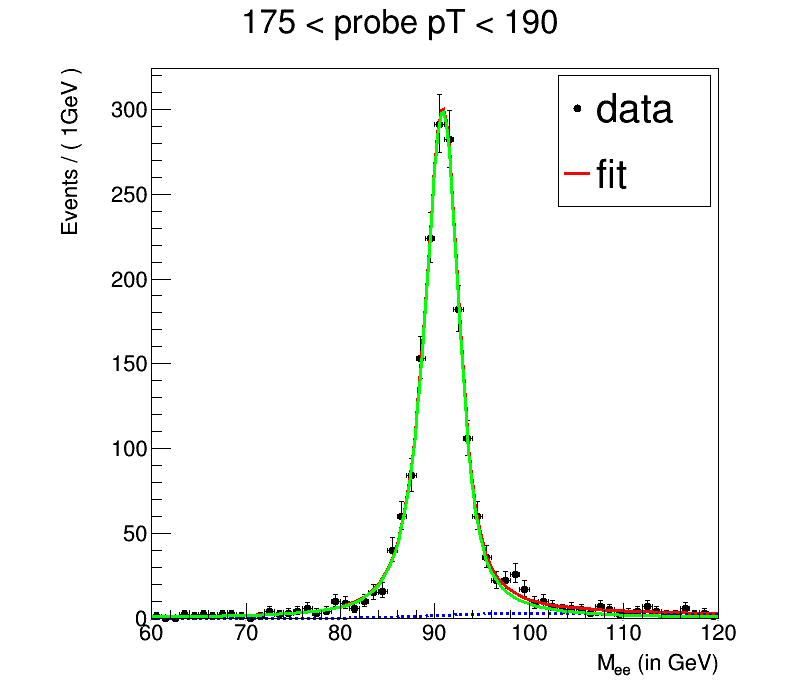
\includegraphics[width=0.40\linewidth]{Figures/efake/EE175190.png}
    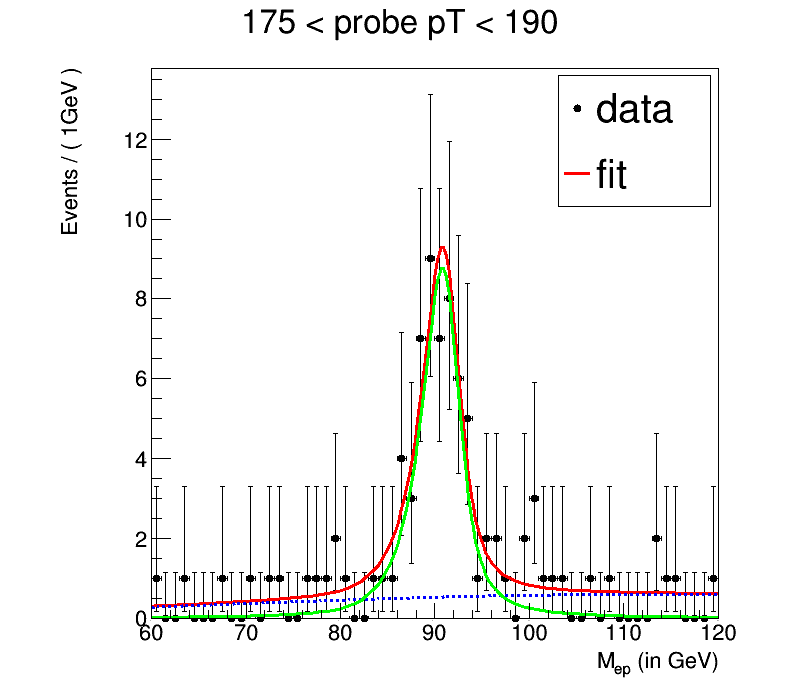
\includegraphics[width=0.40\linewidth]{Figures/efake/EP175190.png}
    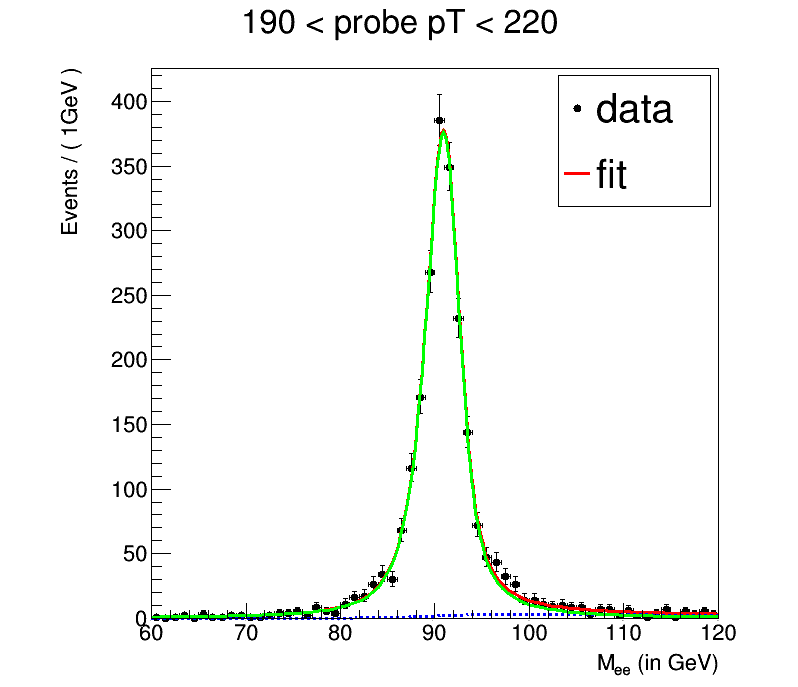
\includegraphics[width=0.40\linewidth]{Figures/efake/EE190220.png}
    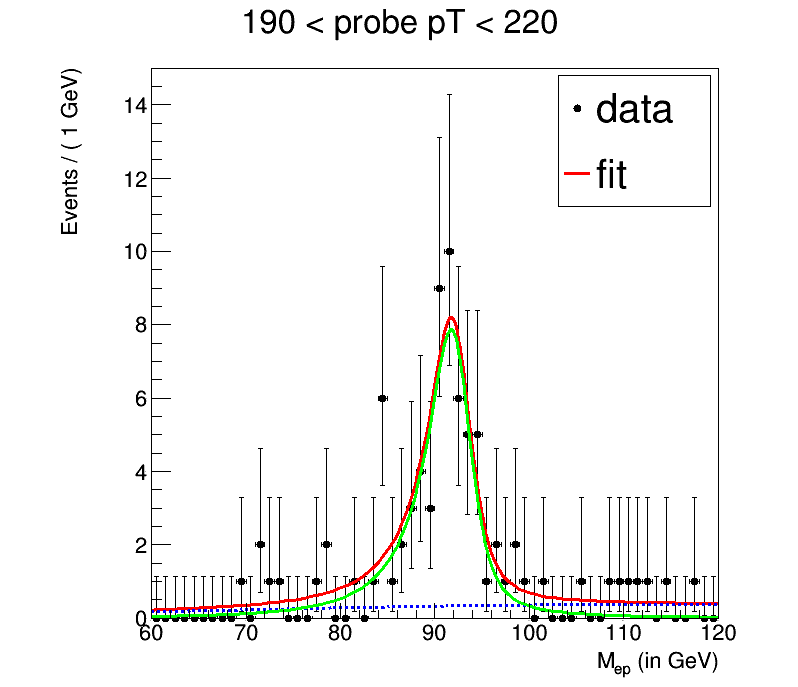
\includegraphics[width=0.40\linewidth]{Figures/efake/EP190220.png}
    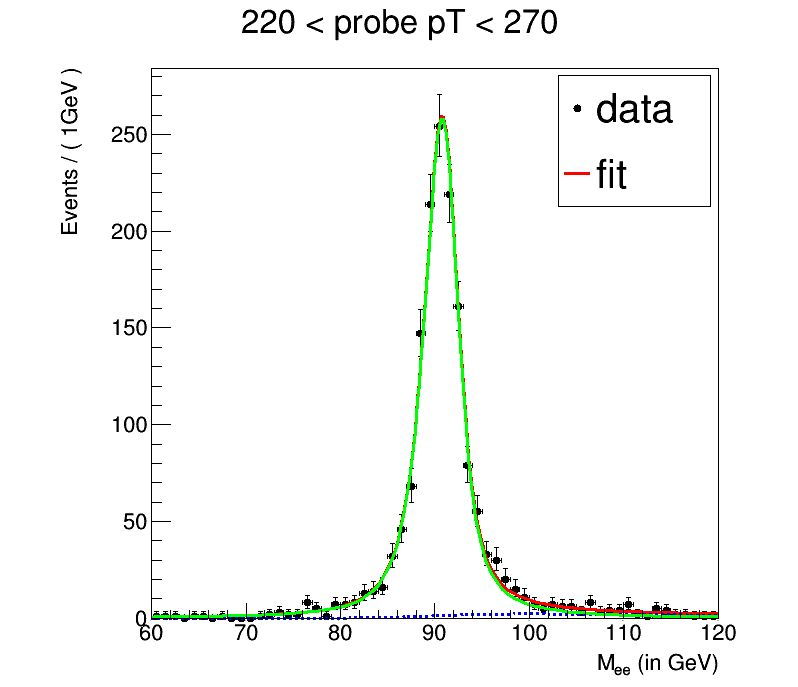
\includegraphics[width=0.40\linewidth]{Figures/efake/EE220270.png}
    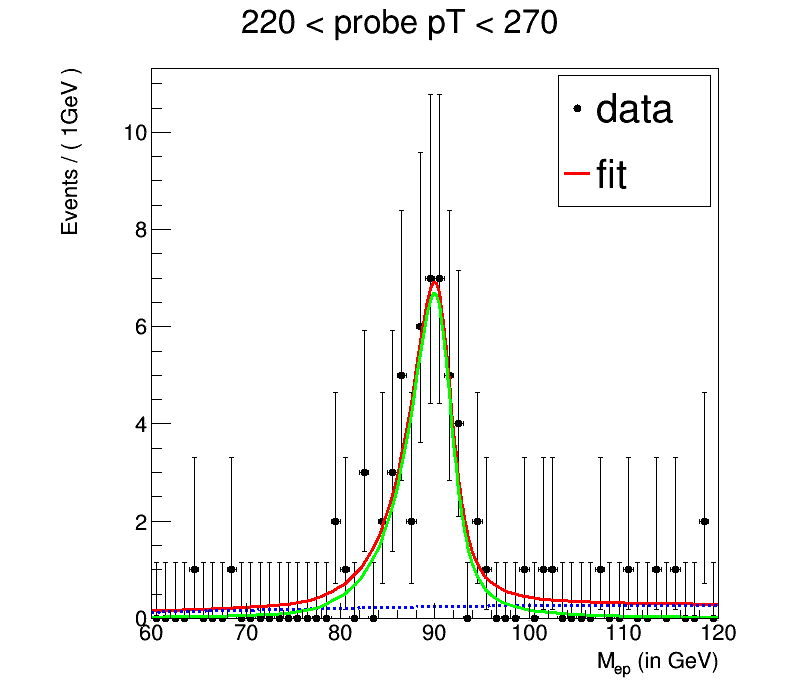
\includegraphics[width=0.40\linewidth]{Figures/efake/EP220270.png}
    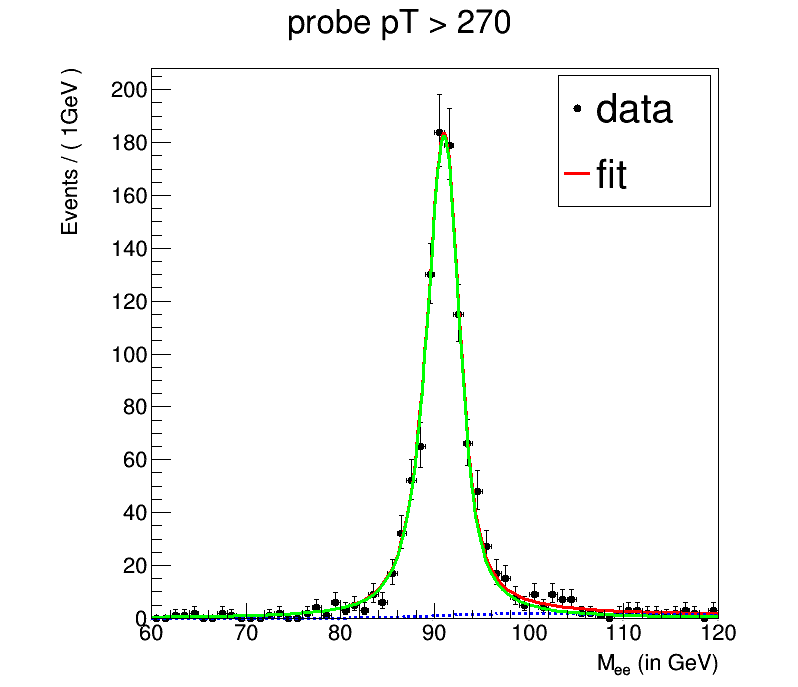
\includegraphics[width=0.40\linewidth]{Figures/efake/EE270.png}
    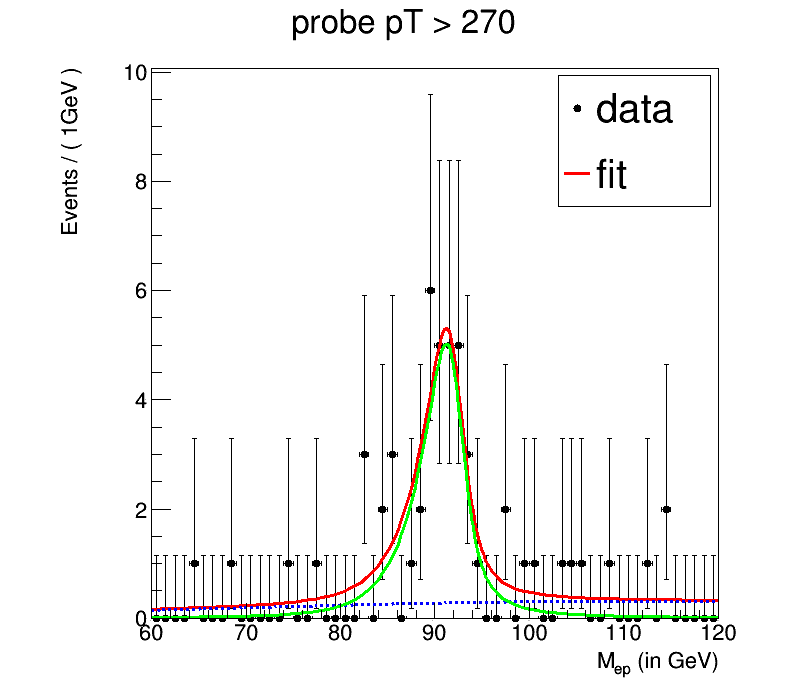
\includegraphics[width=0.40\linewidth]{Figures/efake/EP270.png}
    \caption{
      Fits to the mass distributions for $\Pe\Pe$ (left) and $\Pe\gamma$ (right) selections, in bins of probe \pT: $175 < \pT < 190\unit{GeV}$ , $190 < \pT < 220\unit{GeV}$ , $220 < \pT > 270\unit{GeV}$  and $ \pT > 270\unit{GeV}$.
      The blue dashed curve is the background template, and the red solid curve is the sum of the signal and background templates.
    }
    \label{fig:efake_fits}
  \end{center}
\end{figure}

To estimate the statistical uncertainty on $R_{\Pe}[j]$, 100 samples of random ``toy'' $\PZ{\rightarrow}\Pe\Pe$ events are generated using
the signal template as the underlying distribution. The samples each have the same number of events as the original data sample.
For each sample, the fit is redone using the toy mass distribution as the ``observed'' distribution. The
statistical uncertainty on $R_{\Pe}[j]$ is then taken to be the standard deviation of the toy $R_{\Pe}[j]$ estimates.
The systematic uncertainties on $R_{\Pe}[j]$ are estimated by redoing the fits with alternative signal and background templates.
The alternative signal template is taken from a $\PZ{\rightarrow}\Pe\Pe$ MC sample, and the alternative background template is a second
order polynomial function. The systematic uncertainty from each type of variation is taken to be the shift in the fit result following the variation.
This source of uncertainty is dominated by the signal template uncertainty.

The values of $R_{\Pe}[j]$, along with their uncertainties, are shown in Table~\ref{tab:efake}.
The fake ratio does not appear to vary significantly with \ETgamma.
Under the assumption that the fake ratio is essentially constant, a flat line is fit to $R_{\Pe}[j]$ as a function of \ETgamma. The resulting
y-intercept of 0.03031 is taken to be the constant value of $R_{\Pe}$ for all \ETgamma, with a combined uncertainty of 0.00220.
To estimate the number of events where electrons fake photons in all respects, events are first selected with reconstructed photons
that pass all the photon ID cuts, except that they have matching pixel seeds, and the number of such events is multiplied by
by $R_{\Pe}$.

\begin{table}
  \begin{center}
    \caption{$R_{\Pe}$ and its relative statistical and systematic uncertainties, as a function of probe \pT.}
    \label{tab:efake}
    \begin{tabular}{| c | c | c | c|}
      \hline
      Probe \pT\ [GeV] & $R_{\Pe}$ & Statistical (\%)  & Systematic (\%)  \\
      \hline
      \hline
      $[175, 190]$ &  0.032 & 12.3 & 4.4 \\
      \hline
      $[190, 220]$ & 0.027 & 11.1 & 8.2 \\
      \hline
      $[220, 270]$ &  0.031 & 12.2 & 3.6 \\
      \hline
      $[270, inf]$ &  0.034 & 14.9 & 12.6 \\
      \hline
    \end{tabular}
  \end{center}
\end{table}

\section{Jet faking photon} \label{sec:background_estimation_jetfake}
Like the electron faking photon background, the expected jet faking photon background is estimated via a data-driven method employing a fake ratio.
The numerator of the fake ratio should be the number of fake photon events originating from jets (passing any given signal or control region definition), and so
is defined by selecting events with a leading photon passing our standard photon ID.
The denominator should the number of events in which a high-\ET\ reconstructed photon is surrounded by so much energy from other particles
that it fails a loose set of isolation criteria (and so the photon is likely a jet constituent rather than a true hard-process photon); it is defined by selecting events
with a photon failing a relatively loose ID that has a 90\% selection efficiency for real photons\footnote{Denominator events must still pass a
``very loose'' ID with five times higher maximum isolation cuts.}.

The fake ratio is esimated by counting the number of numerator and denominator events in a control region defined by $\MET < 30\unit{GeV}$. Both the observed
numerator and denominator yields are expected to receive ``contamination'' from real hard-process photon events. The expected contribution of real hard-process
photons to the observed numerator yield is estimated (and subtracted out) by fitting real and fake photon templates to the photon \sieie\ distribution of numerator
events. The real photon template is estimated using \gjets\ MC. The fake photon template is derived from observed event yields in a \textit{sideband} region in which
the leading photon has worst charged hadron isolation lying between 8 and 14\unit{GeV}, but otherwise passes numerator cuts.
This sideband was chosen for the relative absence of real photon contamination. Nevertheless, some residual real photon events are still expected to contribute, and
the fake template is finally ``cleaned'' by subtracting the expected \sieie\ distribution of real photon events estimated in \gjets\ MC.

\begin{figure}[hbtp]
  \begin{center}
  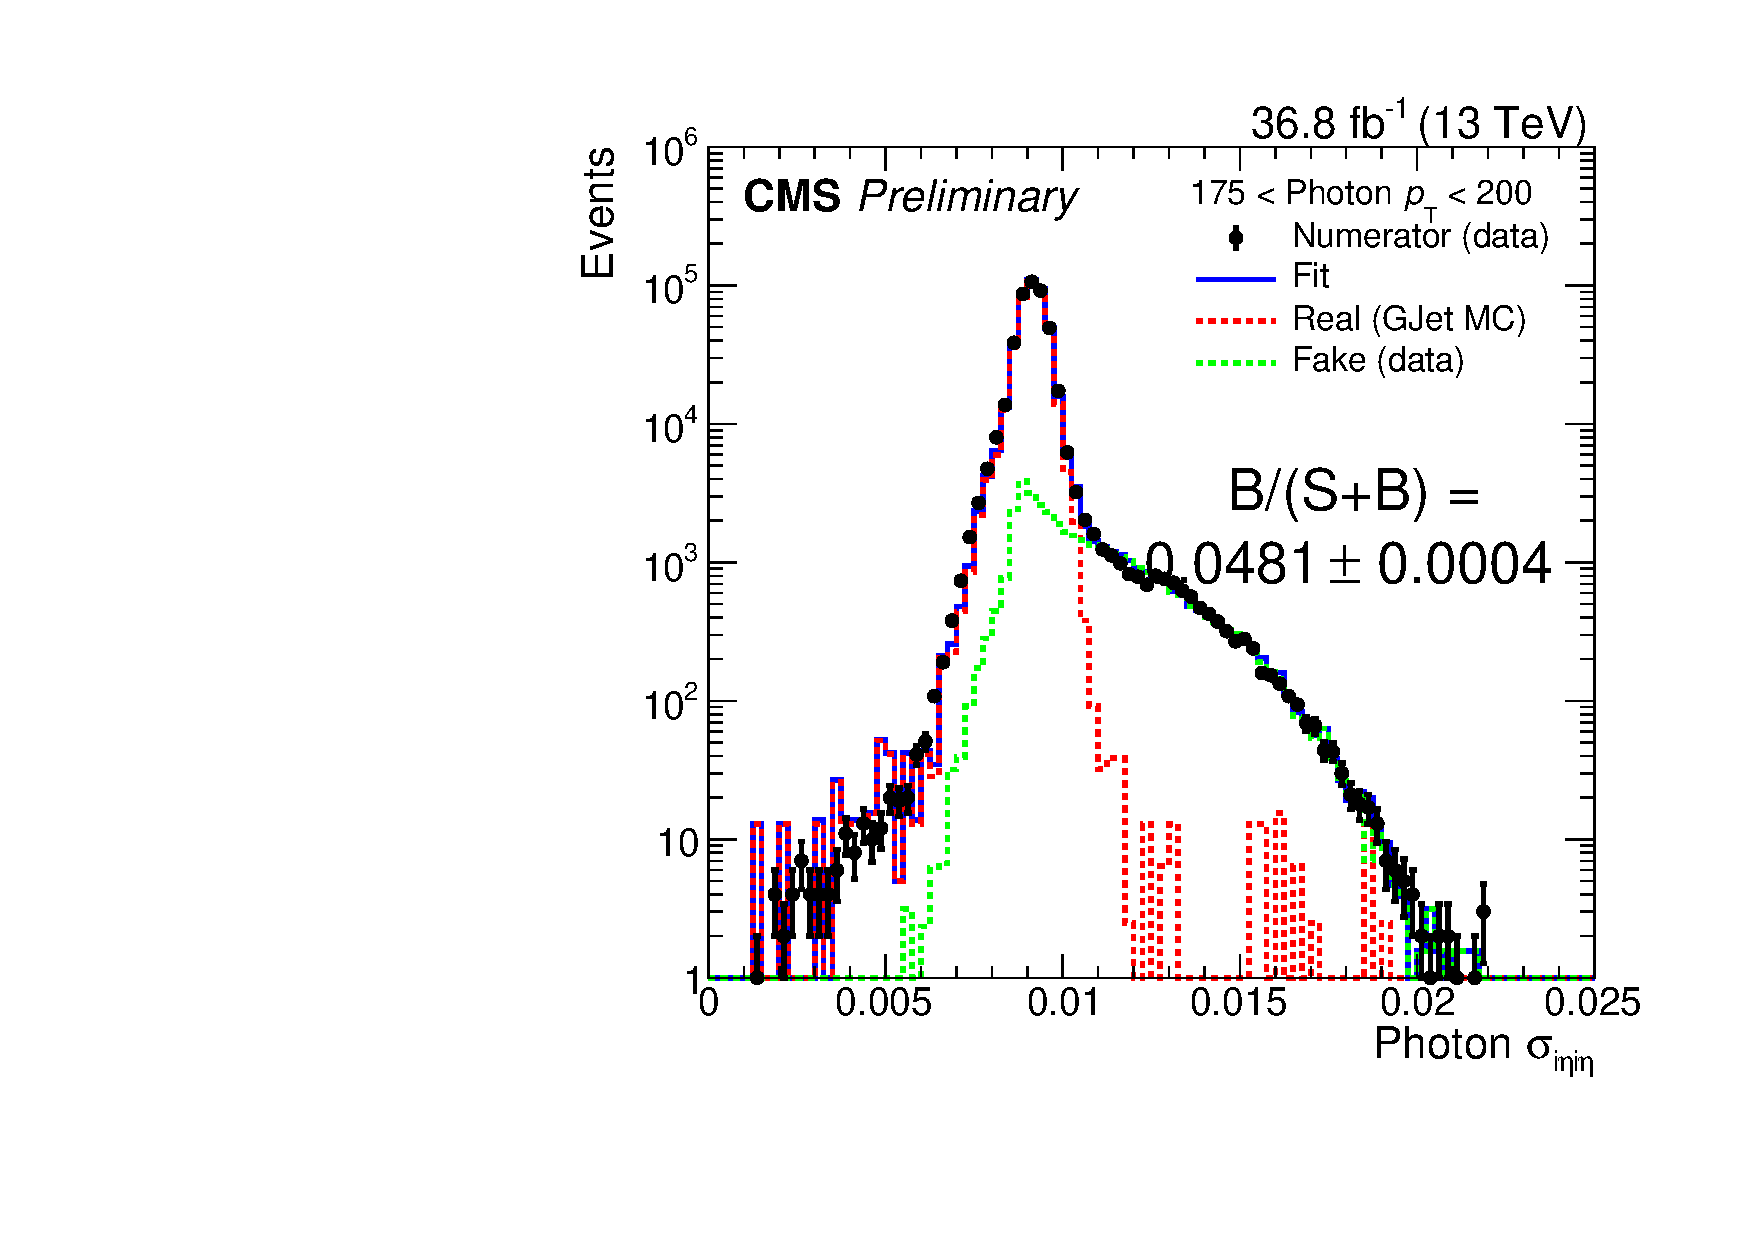
\includegraphics[width=0.45\textwidth]{Figures/QCD/num_fit_175to200.pdf}
  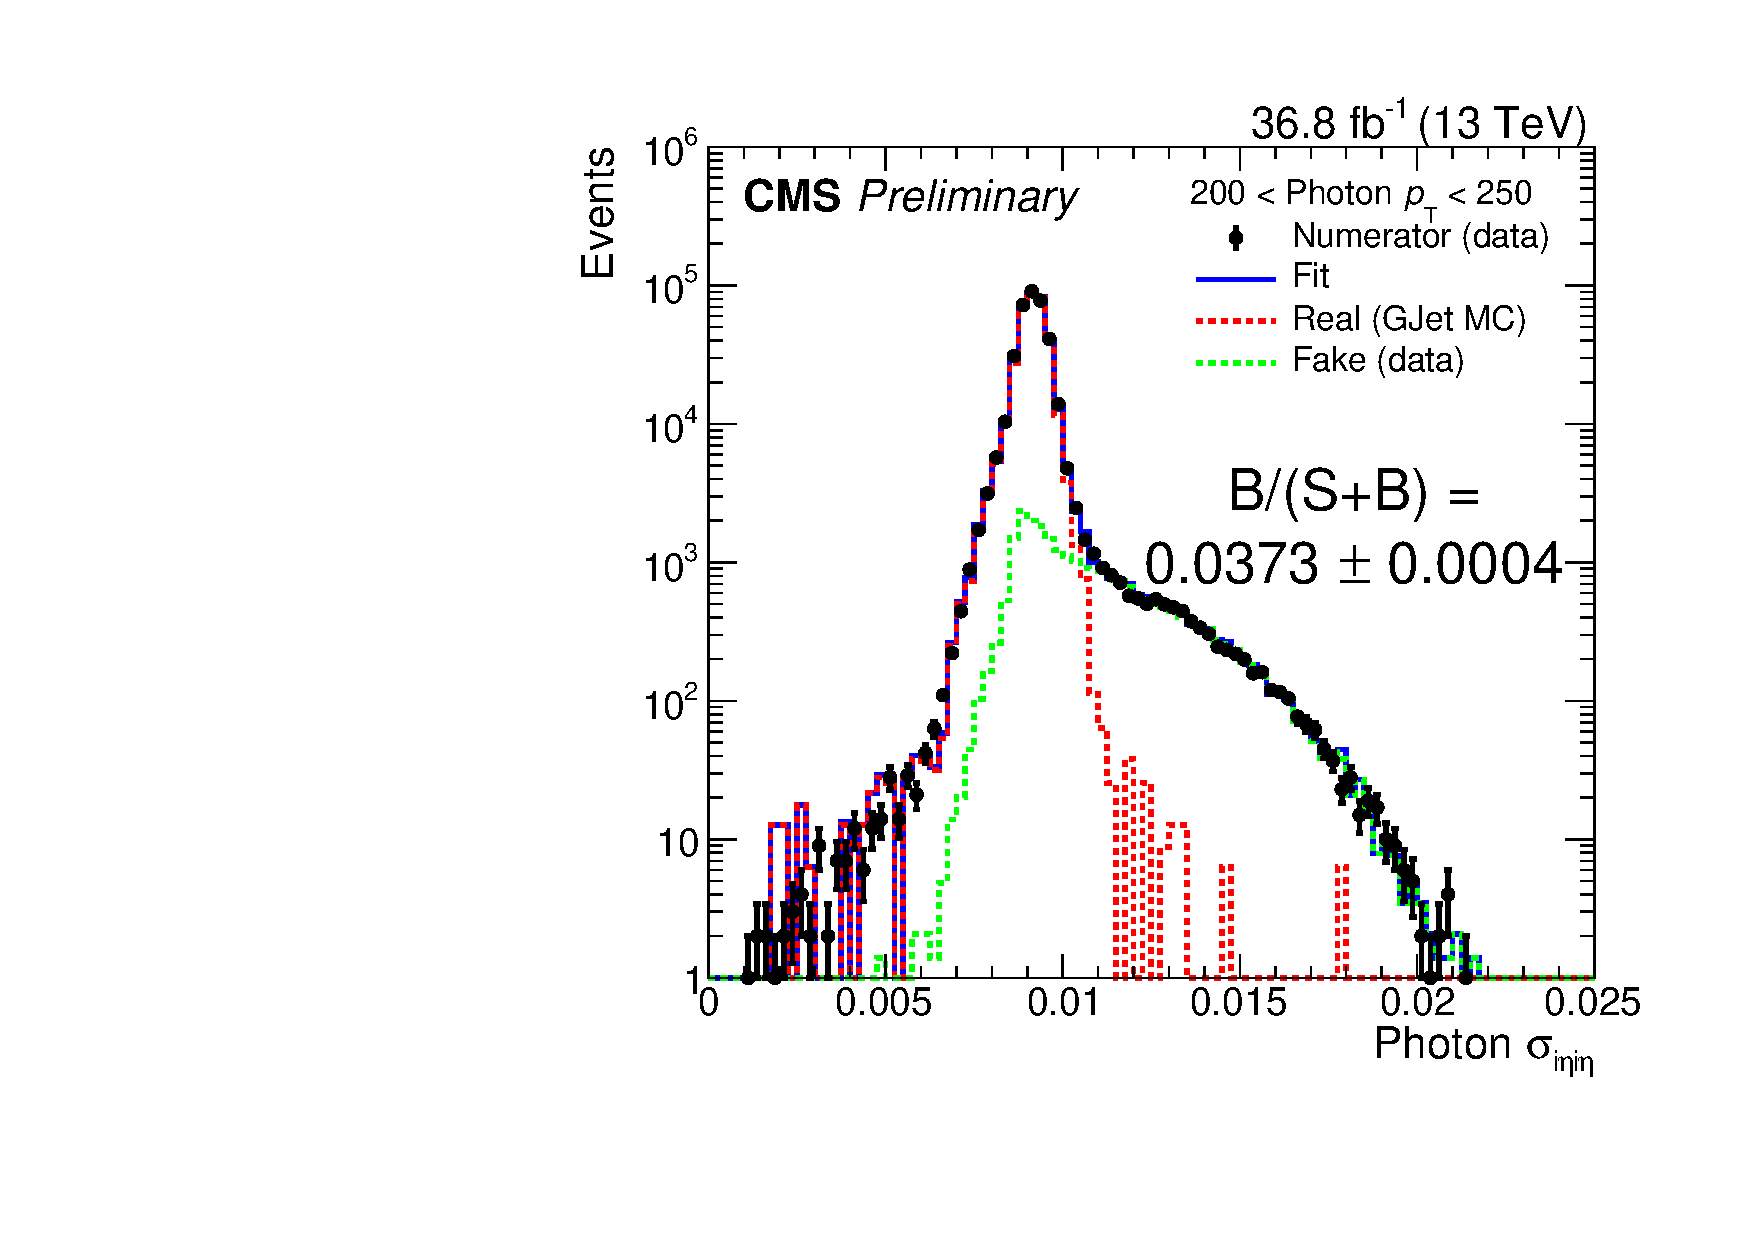
\includegraphics[width=0.45\textwidth]{Figures/QCD/num_fit_200to250.pdf}
  \caption{Distributions of photon $\sigma_{i\eta i\eta}$ in data, and fits to real and fake photon components, in \ETgamma\ bins 175-200\unit{GeV} and 200-250\unit{GeV}.
  The template fitting is done over the whole \sieie\ distribution seen here, and then the fake ratio numerator is computed by integrating the fake photon template (green)
  from 0 to 0.0104, corresponding to the monophoton ID cut. B/(S+B) refers to the fraction of fake events compared to all observed numerator events within this region of integration.}
  \label{fig:qcd_fits_a}
  \end{center}
\end{figure}

\begin{figure}[hbtp]
  \begin{center}
  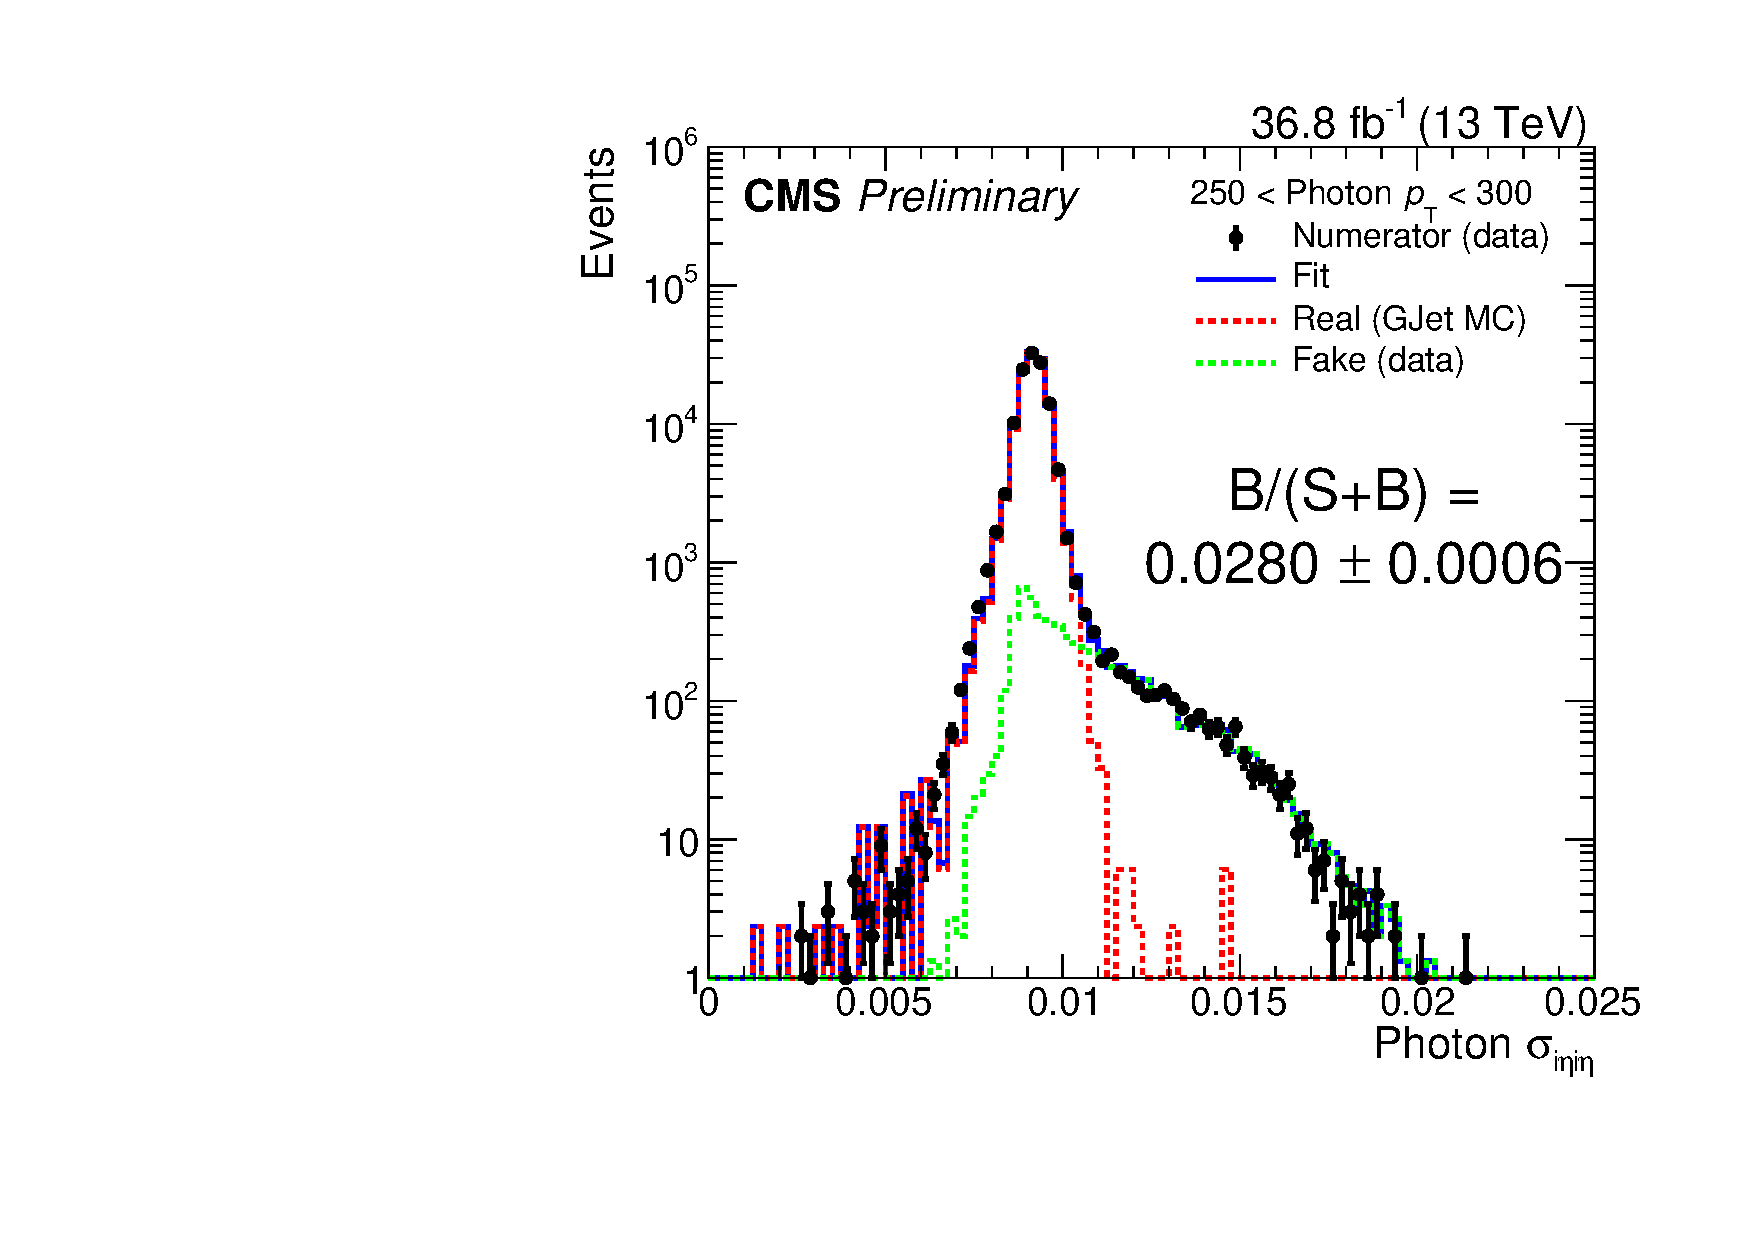
\includegraphics[width=0.45\textwidth]{Figures/QCD/num_fit_250to300.pdf}
  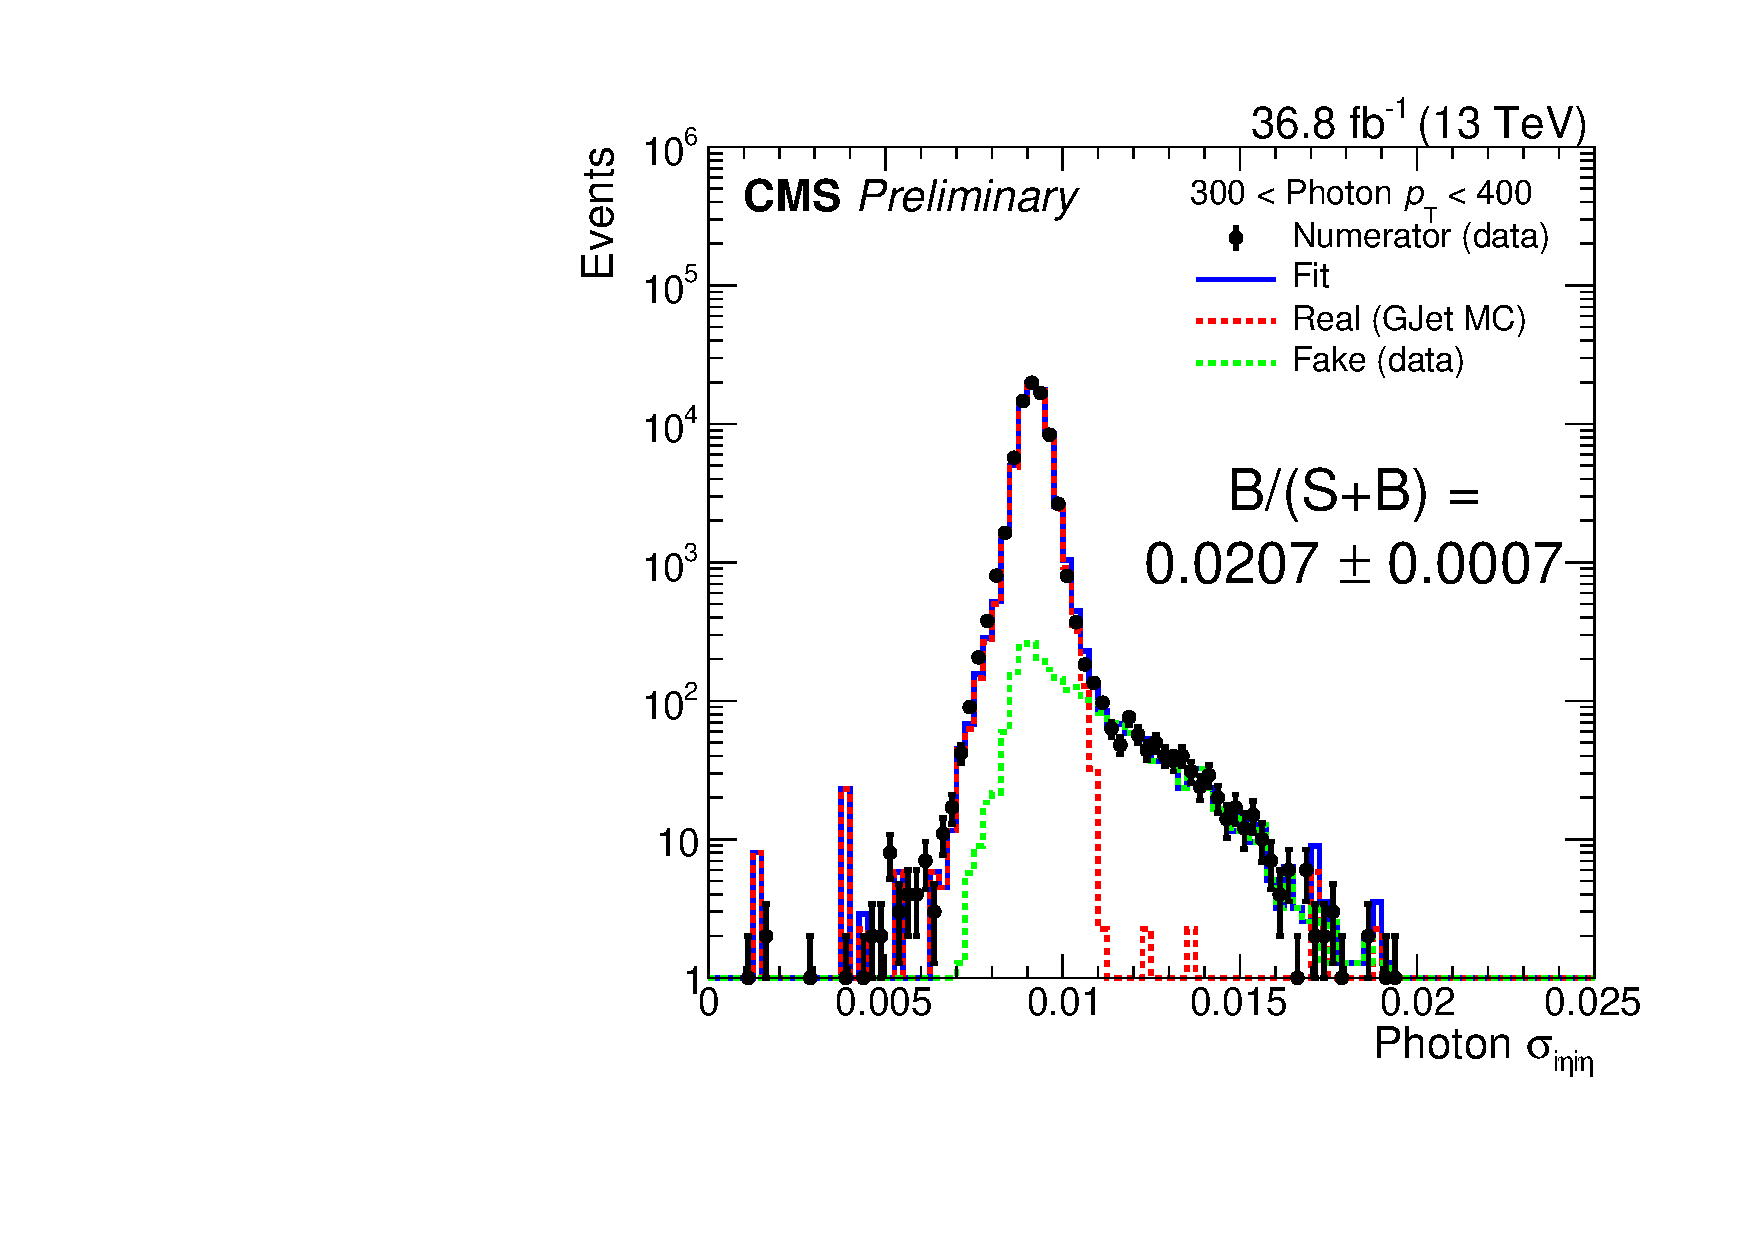
\includegraphics[width=0.45\textwidth]{Figures/QCD/num_fit_300to400.pdf}
  \caption{Distributions of photon $\sigma_{i\eta i\eta}$ in data, and fits to real and fake photon components, in \ETgamma\ bins 250-300\unit{GeV} and 300-400\unit{GeV}.
  The template fitting is done over the whole \sieie\ distribution seen here, and then the fake ratio numerator is computed by integrating the fake photon template (green)
  from 0 to 0.0104, corresponding to the monophoton ID cut. B/(S+B) refers to the fraction of fake events compared to all observed numerator events within this region of integration.}
  \label{fig:qcd_fits_b}
  \end{center}
\end{figure}

\begin{figure}[hbtp]
  \begin{center}
  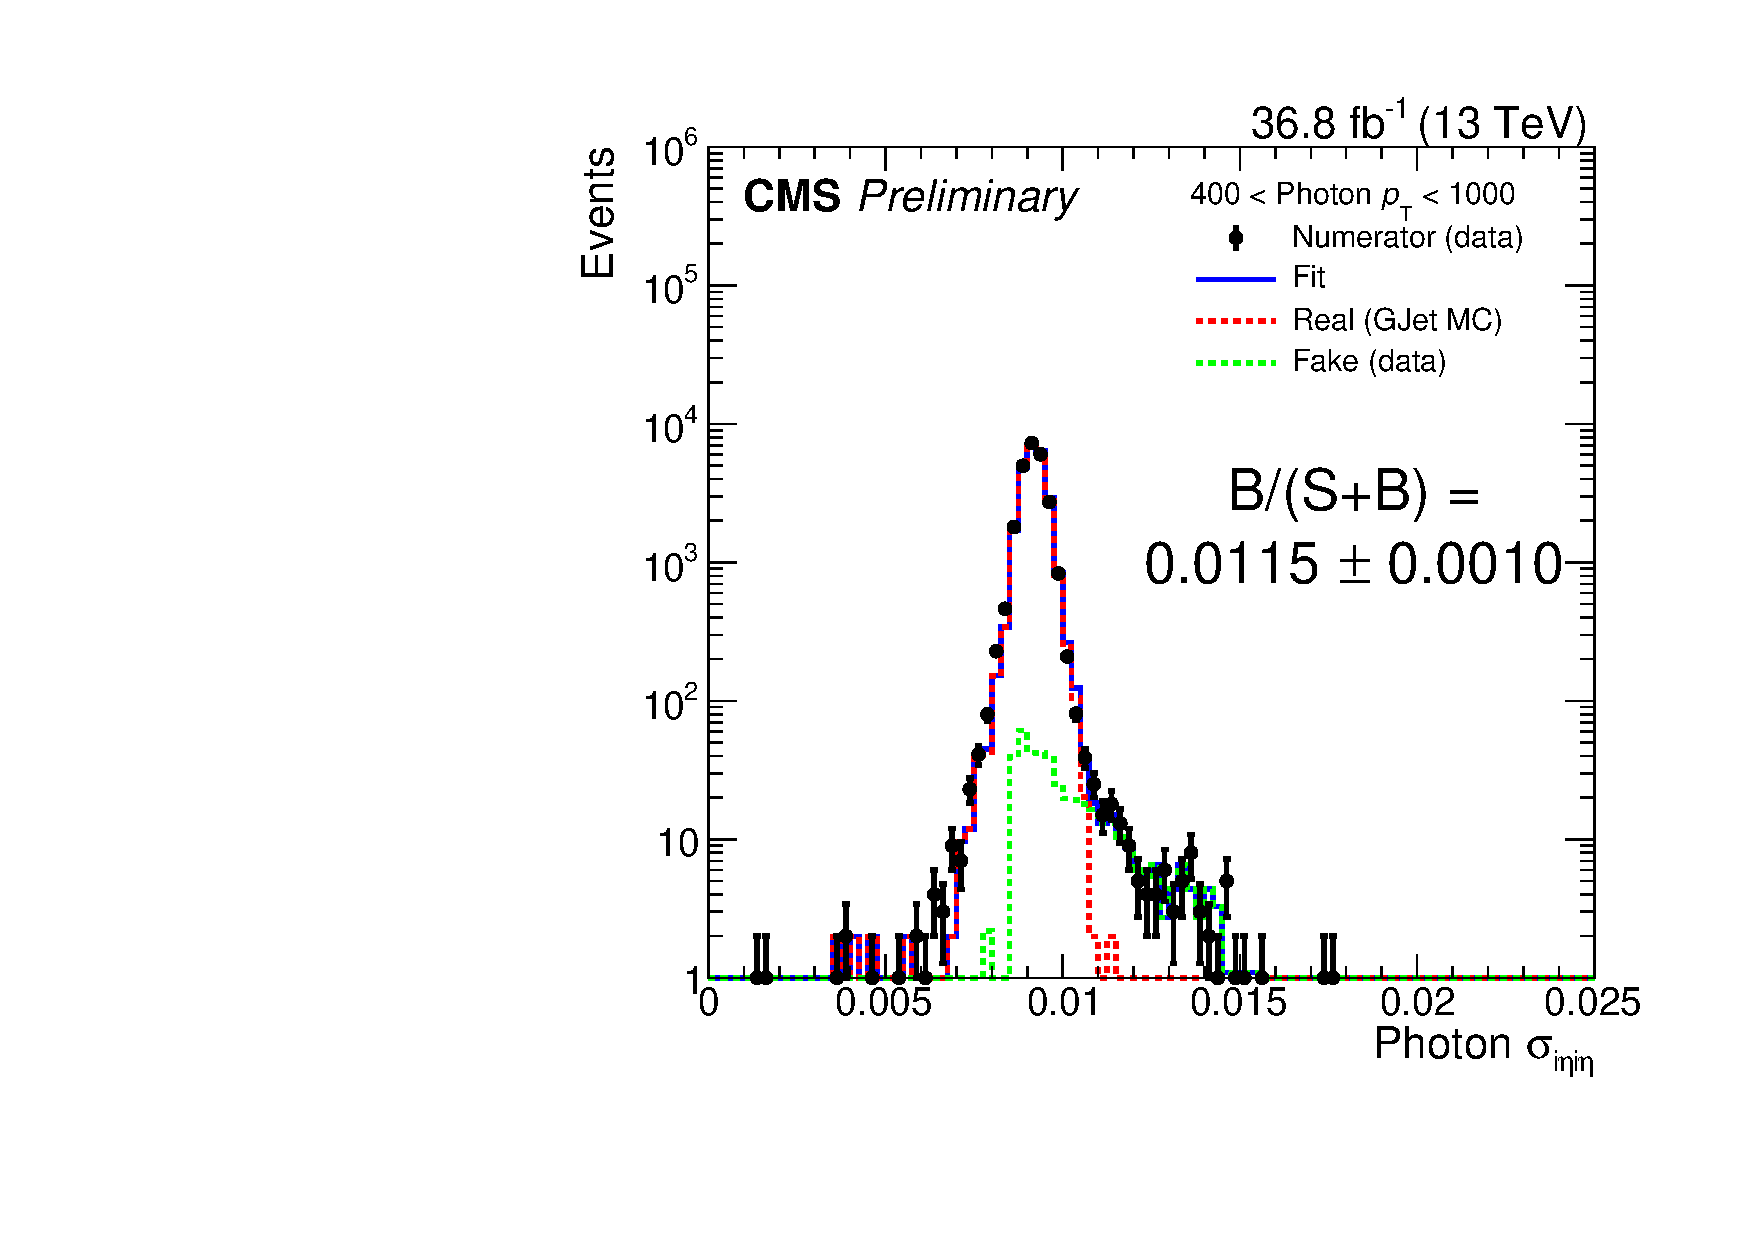
\includegraphics[width=0.45\textwidth]{Figures/QCD/num_fit_400to1000.pdf}
  \caption{Distributions of photon $\sigma_{i\eta i\eta}$ in data, and fits to real and fake photon components, in \ETgamma\ bin 400-1000\unit{GeV}.
  The template fitting is done over the whole \sieie\ distribution seen here, and then the fake ratio numerator is computed by integrating the fake photon template (green)
  from 0 to 0.0104, corresponding to the monophoton ID cut. B/(S+B) refers to the fraction of fake events compared to all observed numerator events within this region of integration.}
  \label{fig:qcd_fits_c}
  \end{center}
\end{figure}

The above procedure ensures a robust estimate of the fake photon yield in the numerator within the $\MET < 30\unit{GeV}$ control region.
The fake photon yield must also be estimated in the denominator, with the
additional constraint that it must be estimated in the same way both in the $\MET < 30\unit{GeV}$ control region and in any other signal or control regions in which
the final jet faking photon yield is needed. In such other regions, the template fitting method described above is not practicable. Instead, an additional
cut is applied on photon \sieie\ in the denominator to remove any possible real photons, so as to preserve a consistent denominator composition in any control region.
Inverting the \sieie\ cut from the monophoton ID ensures that nearly 100\% of real photon events (as estimated in \gjets\ MC) are removed from the denominator,
while preserving a maximal number of fake photon events.

Both the numerator template fitting and studies of denominator purity depend on having reliable MC estimates of the \sieie\ distribution of real photon events.
Studying the \sieie\ distributions of electrons in tag-and-probe samples in both MC and data reveals a consistent discrepancy between the two, of up to a few percent.
Electrons and photons have very similar \sieie\ distributions, and the data vs. MC discrepancy is believed to be similar
for both types of particles. To correct this discrepancy, the photon \sieie\ shapes obtained in MC are multiplied by the ratio of the electron \sieie\ shape from data
over the corresponding electron \sieie\ shape from MC.

The resulting fake ratio is illustrated in Fig.~\ref{fig:qcd_fake_ratio}.
It is assumed to have approximately the same value regardless of which signal or control region cuts are applied. However, the $\MET < 30\unit{GeV}$ cut
that defines the fake ratio control region is substantially different from the $\MET > 170\unit{GeV}$ cut defining the signal regions, and jets
are complex multiparticle objects that are relatively likely to have mismeasured $\MET$.
To study the possible impact of shifting \MET\ cut definitions on the fake ratio,
the ratio is reevaluated for control regions defined by $\MET < (7/6)\times30\unit{GeV}$ and $\MET < (5/6)\times30\unit{GeV}$.
Other variations in the fake ratio are obtained by shifting the maximum allowed charged hadron isolation in the sideband region up and down by 2\unit{GeV};
shifting the \sieie\ corrections up and down by their uncertainties; and using finer or coarser histogram binning in the numerator templates. Statistical
uncertainties due to limited data and uncertainties stemming from the template fitting procedure are also propagated to the fake ratio. The total uncertainty
on the fake ratio is taken to be the size of the envelope of all of the separate shifts. These shifts are illustrated in Fig.~\ref{fig:qcd_fake_ratio}.

\begin{figure}[hbtp]
  \begin{center}
  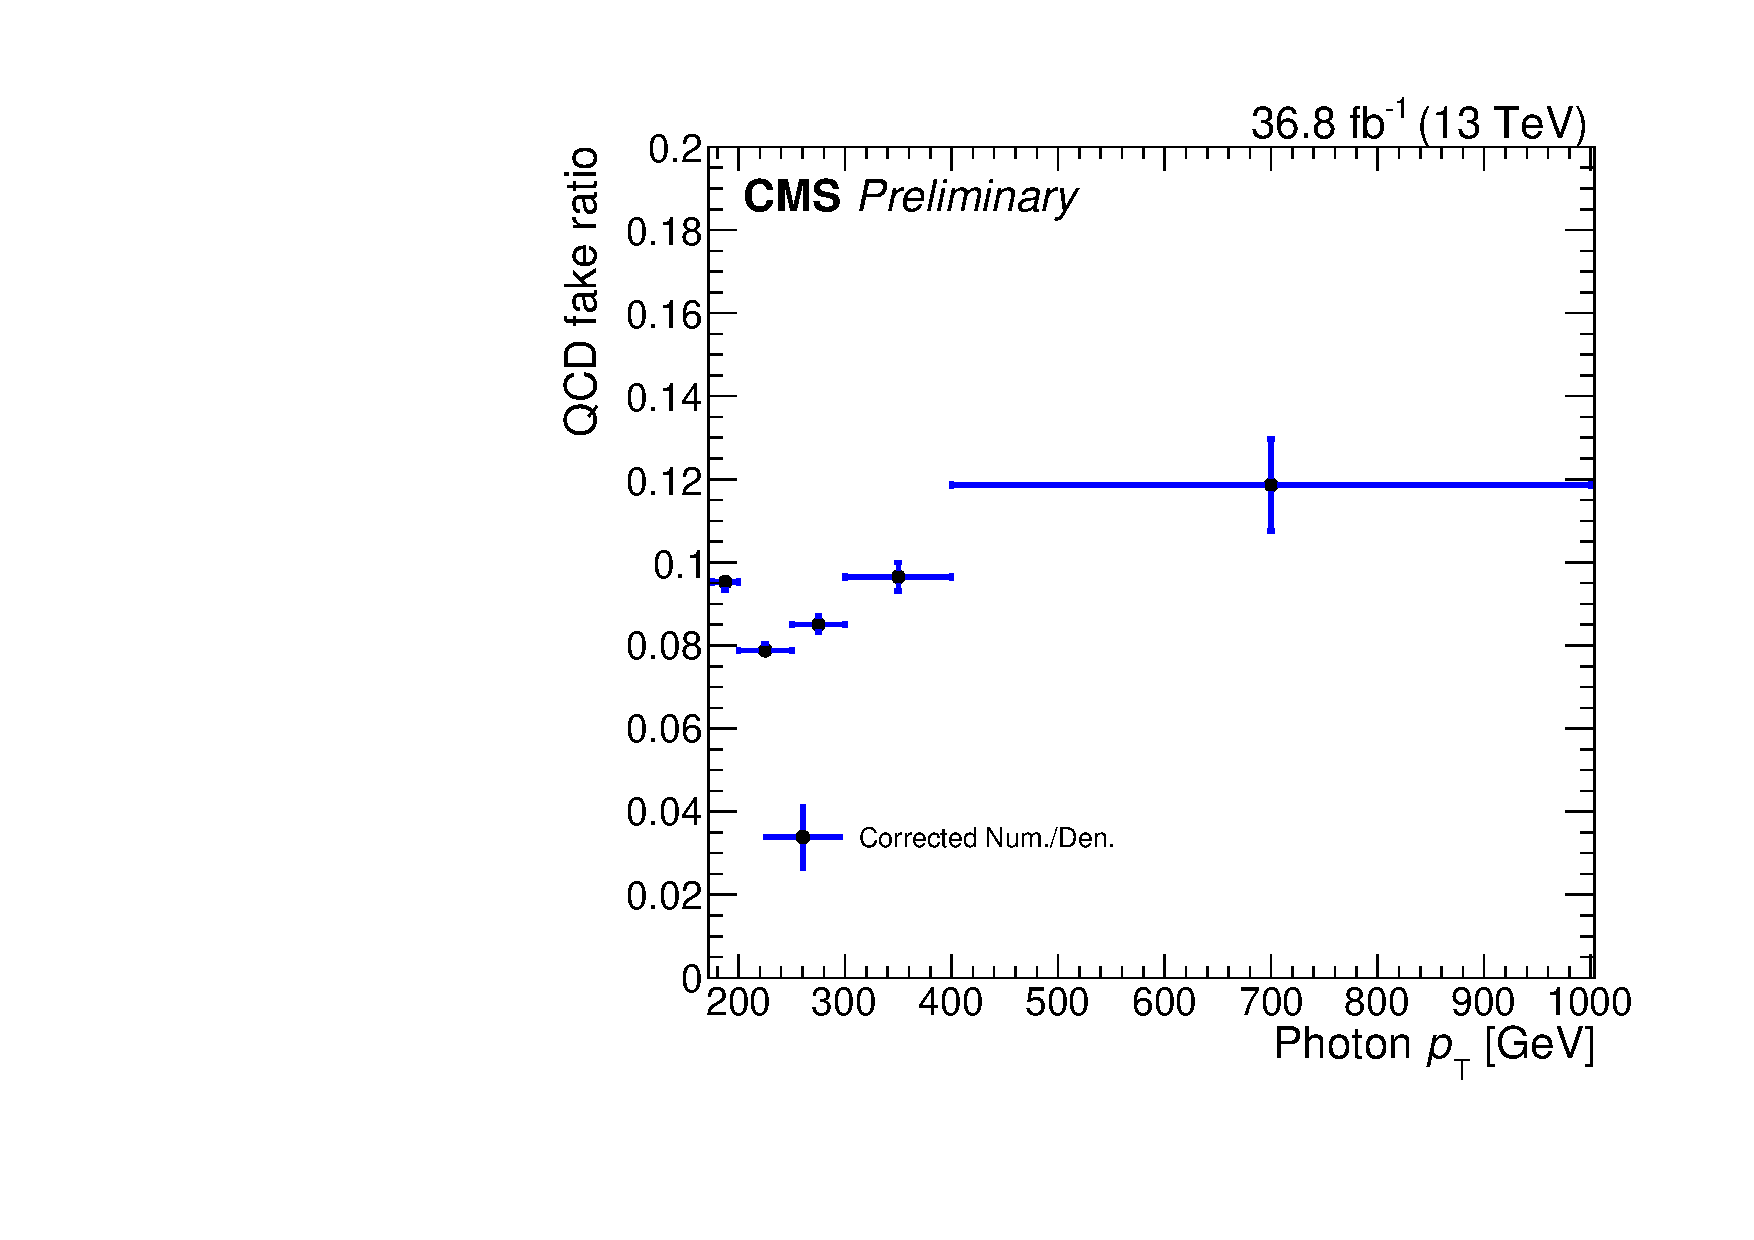
\includegraphics[width=0.45\textwidth]{Figures/QCD/QCDfake_fakeratio.pdf}
  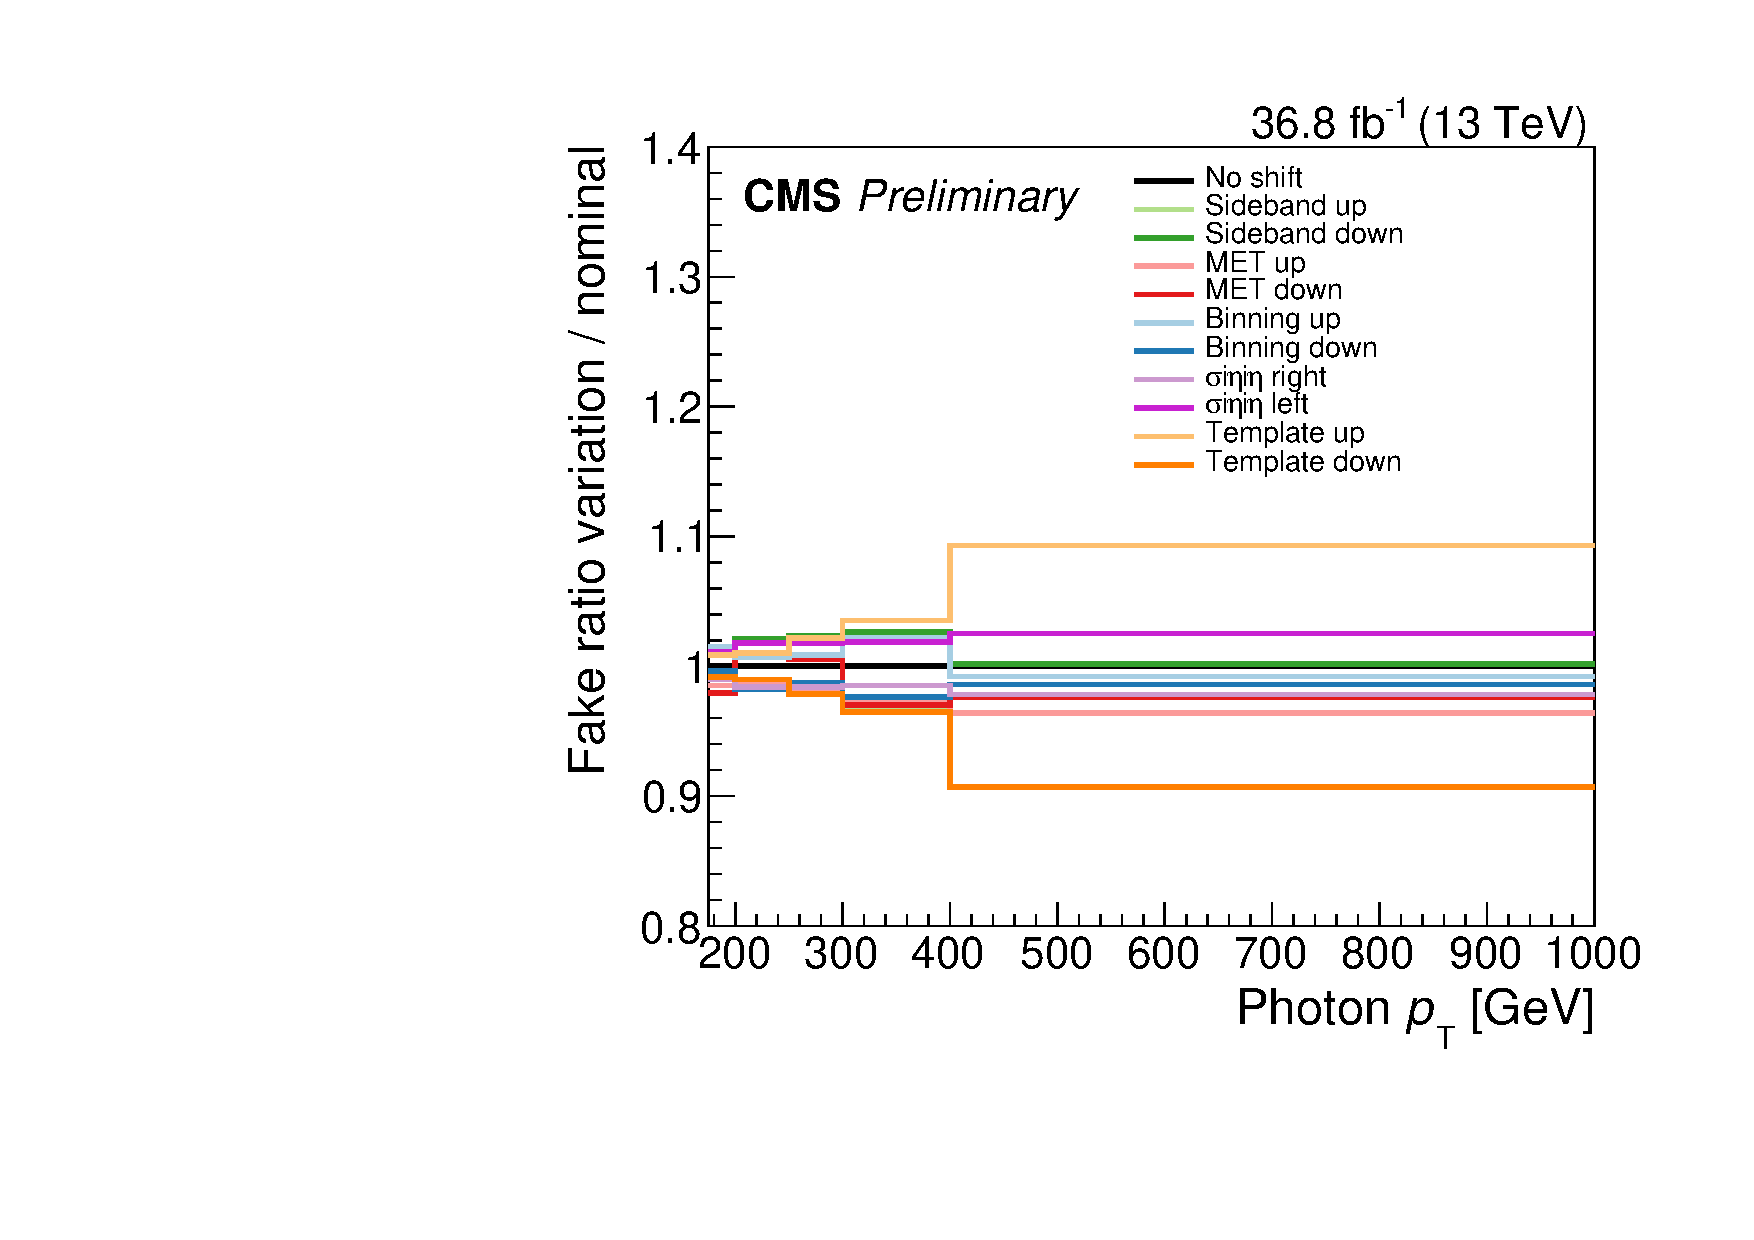
\includegraphics[width=0.45\textwidth]{Figures/QCD/QCDfake_systematics.pdf}
  \caption{The jet fake ratio as a function of \ETgamma\ (left), and fractional variations in that ratio caused by shifts of various types (right).}
  \label{fig:qcd_fake_ratio}
  \end{center}
\end{figure}

\section{Spikes} \label{sec:background_estimation_spikes}
Due to their idiosyncratic means of production, spikes do not currently have simulated samples that could be expected to accurately reproduce their expected yield,
particularly in the case of events somehow passing all the spike cleaning cuts in the monophoton signal regions. Instead, the time distribution of clearly-identified
spikes in observed events can be used to extrapolate the preponderance of spikes within the in-time window ($|t|<3\unit{ns}$) defined by our signal region cuts.
This time distribution is examined by performing a custom reconstruction of the data in which ``spike-killer'' cuts that are part of standard event reconstruction
are omitted. Spike candidates are selected from reconstructed photons that pass a loosened set of ID criteria with no isolation cuts (to account for the different
characteristics of events outside the in-time window) but have $\ETgamma > 175\unit{GeV}$, $\sieie < 0.0104$, and either \sieie\ or $\sipip < 0.1$.
As illustrated in Fig.~\ref{fig:fulltime_templates}, this distribution exhibits a peak around $t = -15\unit{ns}$ and falls off to near zero by the in-time window.

The time distribution of spike candidates is one of three templates used to fit the timing distribution of monophoton-like events from $t = -25\unit{ns}$ to $+25\unit{ns}$,
where a ``monophoton-like event'' is defined to be an event with $\MET > 170\unit{GeV}$ and a reconstructed photon with $\ETgamma > 175\unit{GeV}$ and $0.001 < \sieie < 0.0104$.
candidate events are chosen based on reconstructed photons with MIP total energy greater than 4.9\unit{GeV}. Electron candidate events are chosen based on a
$\PZ{\rightarrow}\Pe\Pe$ tag-and-probe selection similar to that used for the electron fake ratio, in which the probe is a reconstructed photon that has a pixel
seed and serves as the particle whose time is templated. Electron candidates reconstructed as photons have a timing distribution essentially identical to real
photons, with the added advantage that other information in the event (such as the pixel seed) marks these as originating directly from the hard collision process.
The three templates and their fit to the full time distribution are shown in Figs.~\ref{fig:fulltime_templates} and \ref{fig:fulltime}.

\begin{figure}
  \begin{center}
    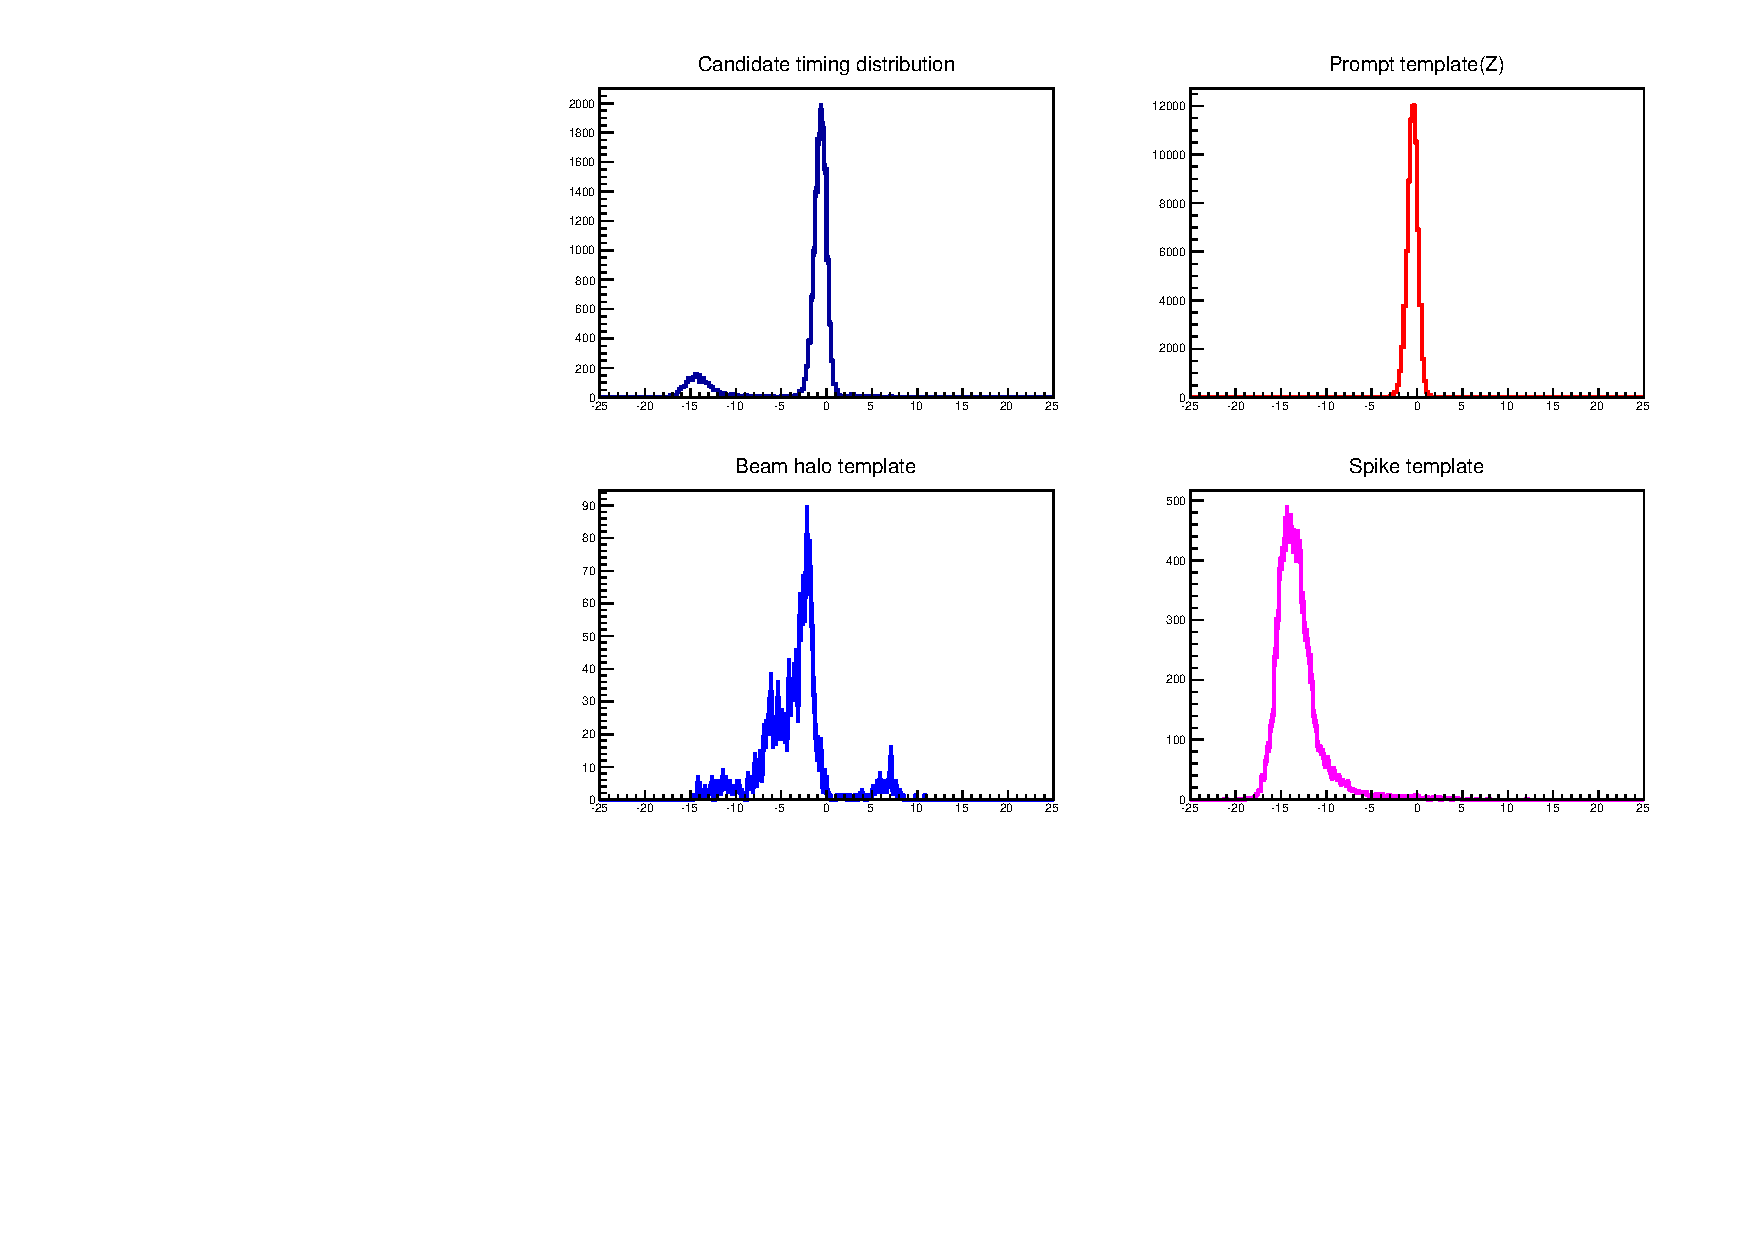
\includegraphics[width=8.0cm,height=6.5cm]{Figures/noncol/TemplatesQuadZ.pdf}
    \caption{
      Time distribution templates for halo, electron, and spike candidates.
    }
    \label{fig:fulltime_templates}
  \end{center}
\end{figure}

\begin{figure}[tbp]
  \begin{center}
    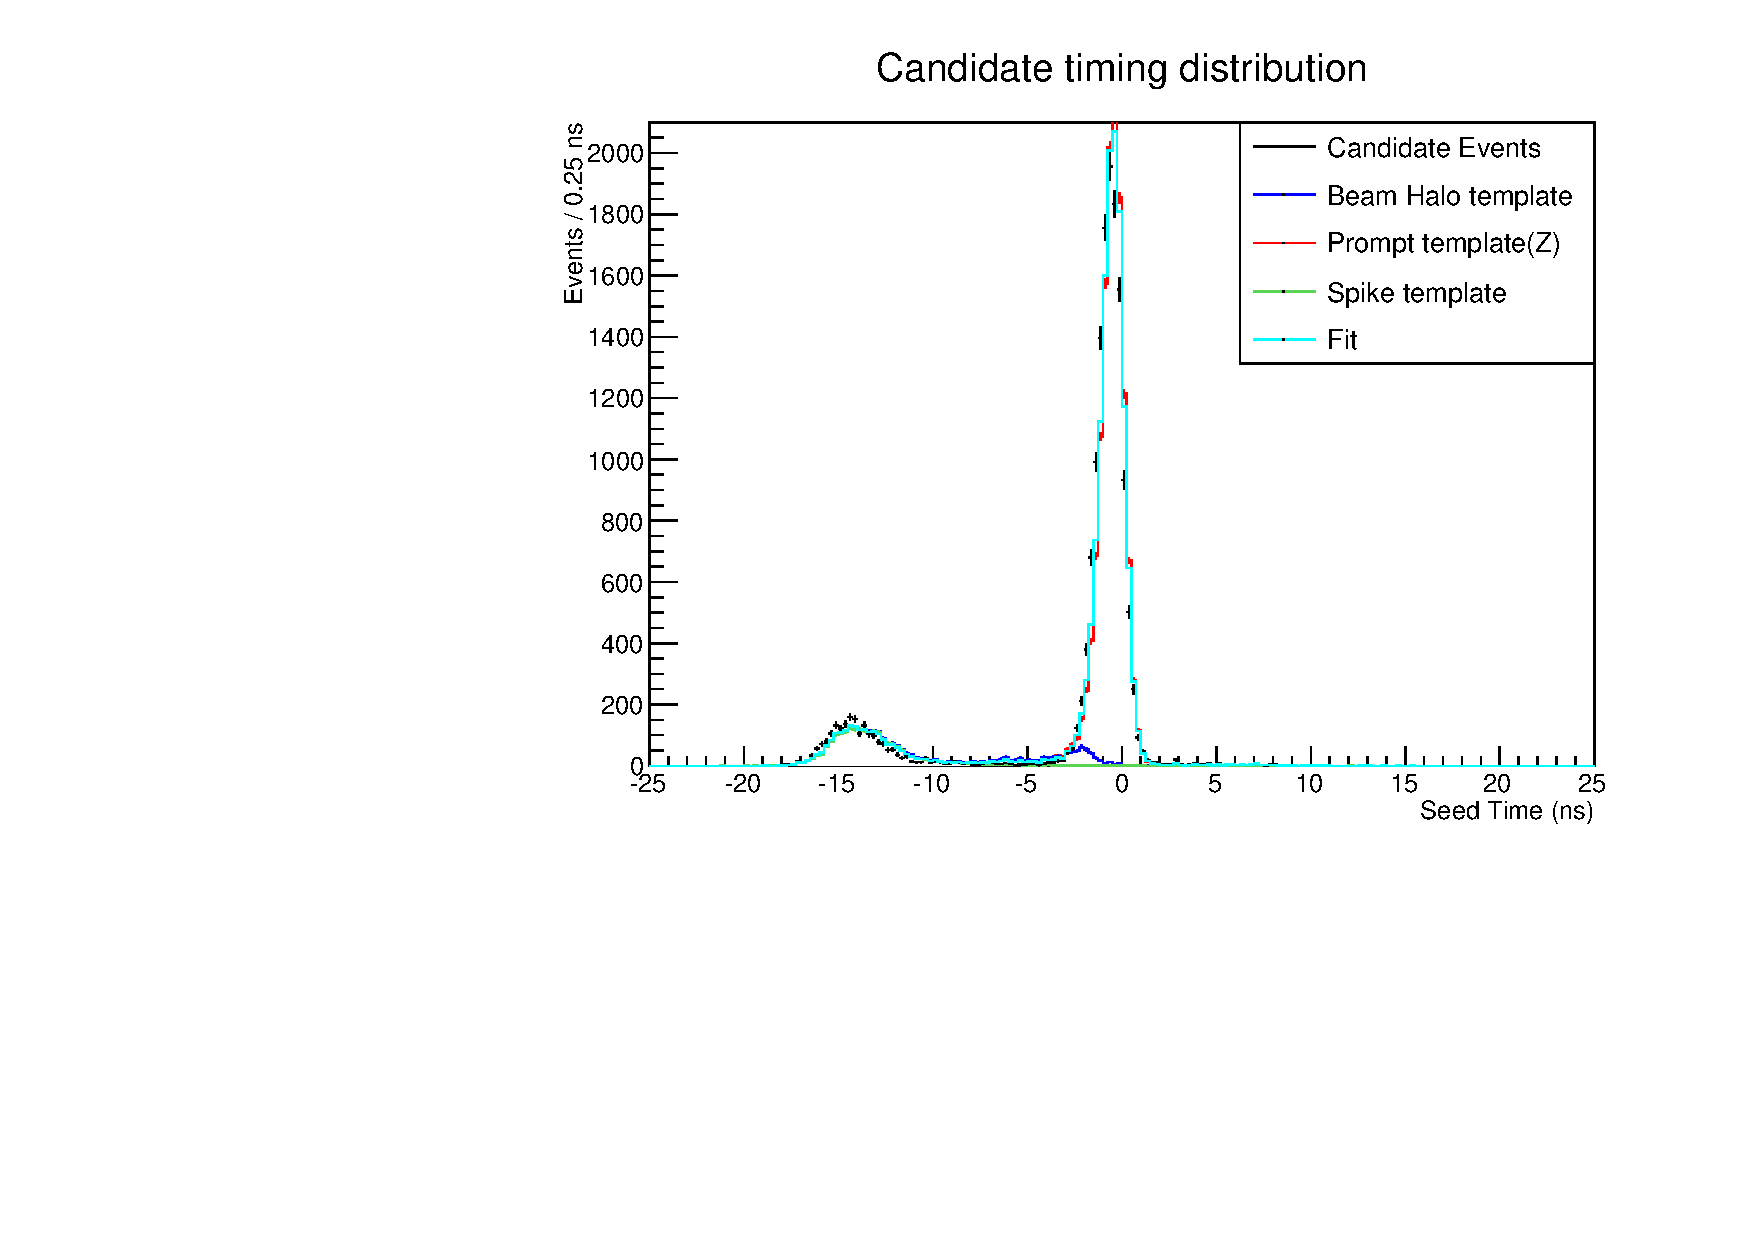
\includegraphics[width=8.0cm,height=6.5cm]{Figures/noncol/StackFractionFitZ.pdf}
    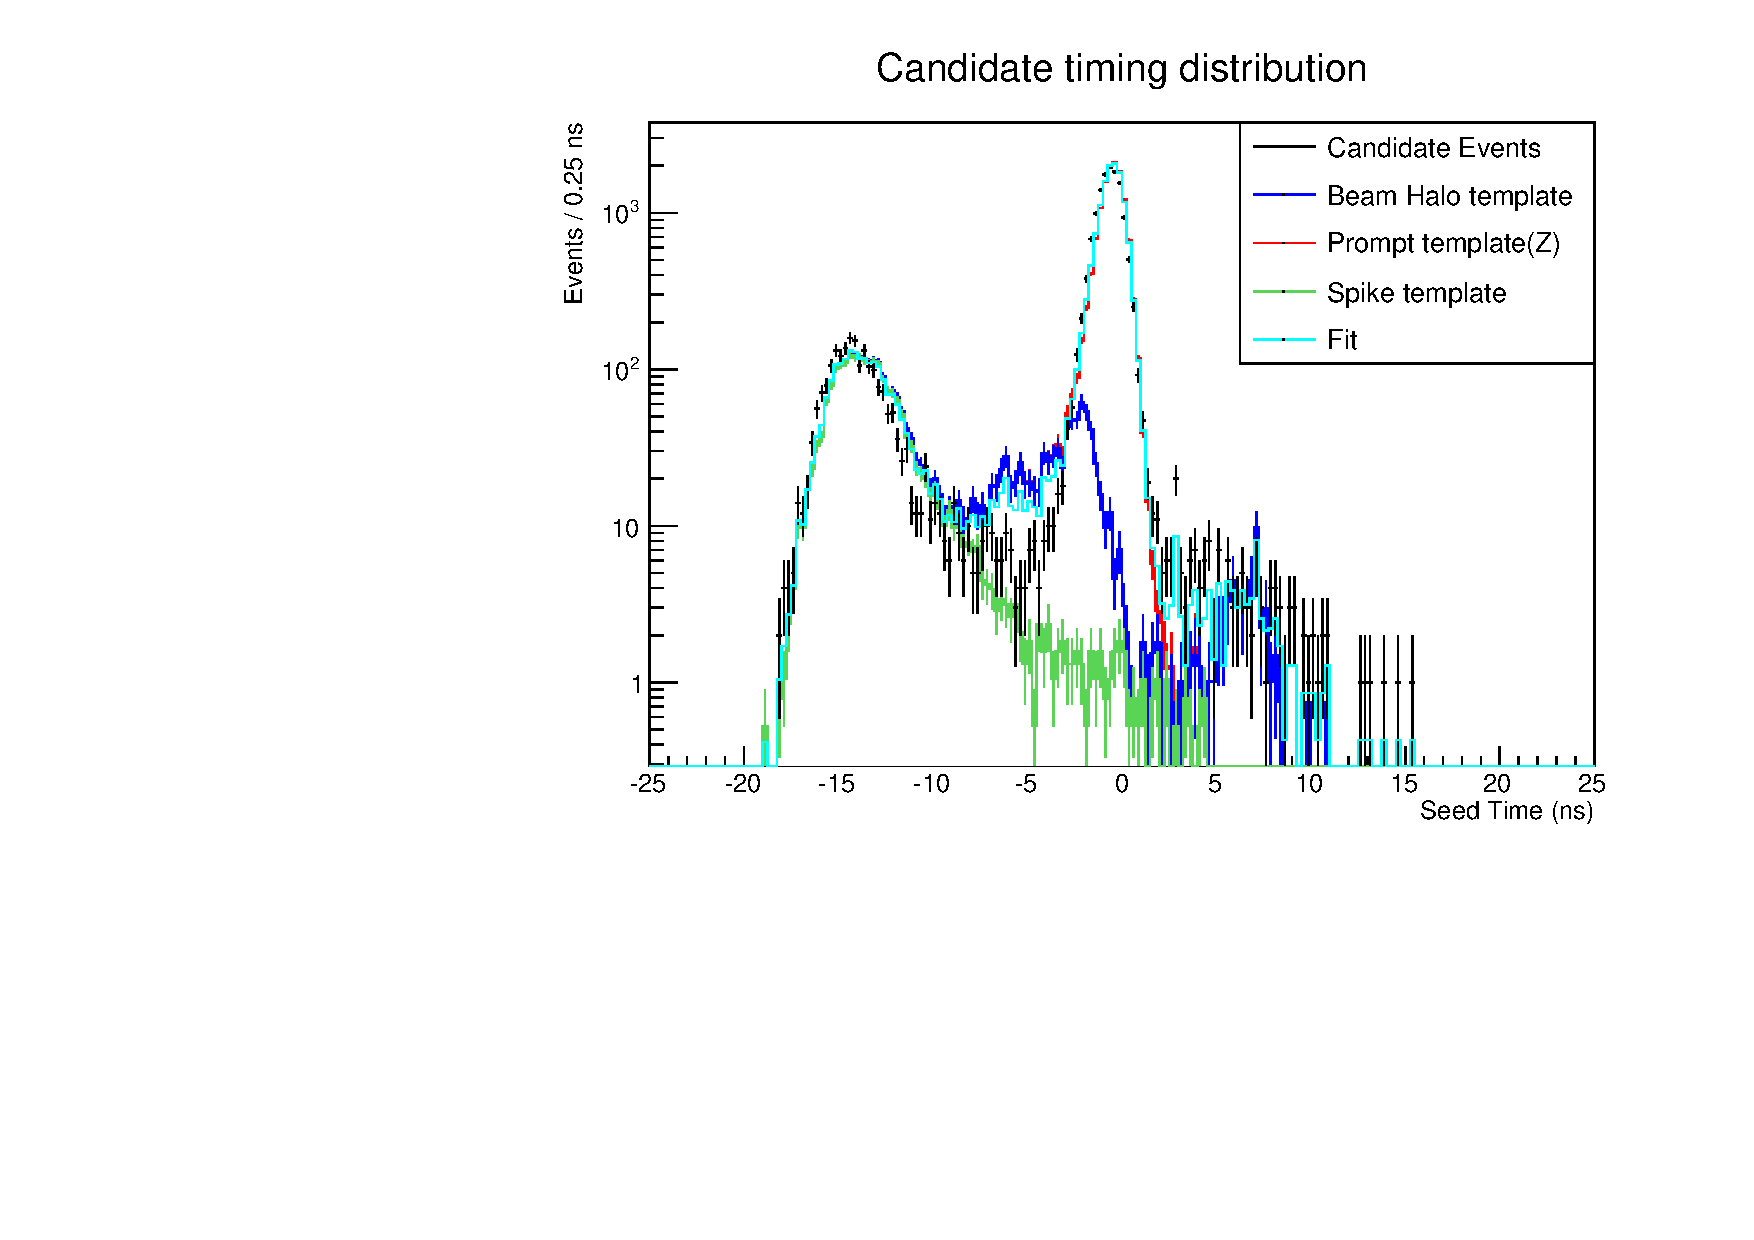
\includegraphics[width=8.0cm,height=6.5cm]{Figures/noncol/StackFractionFitZLog.pdf}
    \caption{
      Observed time distribution of photons with $\ETgamma > 175\unit{GeV}$ and $0.001 < \sieie < 0.0104$ in events with $\MET > 170\unit{GeV}$,
       obtained by a custom reconstruction of 2016 data, shown in linear and log scale.
      The three templates used in the fit are shown in Fig.~\ref{fig:fulltime_templates}.
    }
    \label{fig:fulltime}
  \end{center}
\end{figure}

Due to the lack of isolation cuts on the photon candidates in each template, their integrals within the in-time window are not generally expected to reflect the
expected yield of monophoton events that pass all of the monophoton ID cuts. However, the locations of spikes in the barrel are random and uncorrelated
with respect to the locations of any hard-scatter products, so the probability that a spike would occur in the vicinity of a significant amount of energy deposited
by other particles is negligible. Since the spikes themselves have extremely narrow shower shapes, any isolation sum is therefore expected to be small enough to
pass the monophoton ID. For the same reasons, H/E is expected to be negligible for any spike.
It is thus assumed that, after fitting to the monophoton-like time distribution, the integral of the spike template within the in-time window
represents the expected number of spikes that pass all monophoton ID cuts.

The statistical uncertainty on the timing template fit is 2.5\%, but the expected spike yield can vary by up to 20\% when the templates are defined
in different ways. Alternative spike templates were formed by loosening the \sieie\ cut from 0.001 to 0.002 in units of 0.0001,
and by instead using a maximum cut on $W_{\eta}$, which was varied between 0.010 to 0.017 in steps of 0.001.

An alternative estimate of the spike yield is obtained based on the variable
\begin{equation}
W_{\eta} = \frac{E_{1}}{E_{0}}
\end{equation}
where $E_{0}$ is the energy of the seed crystal of the cluster and $E_{1}$ is the higher of the energies of two crystals adjacent to the seed in $\eta$.
It is expected that spikes should have small $E_{1}$, whereas real showers should have some energy shared between the seed and its neighbors.
Figure~\ref{fig:etawing} shows the distribution of $W_{\eta}$ for observed showers corresponding to
$\PZ{\rightarrow}\Pe\Pe$ candidates and spike candidates (selected using a $t < -12.5\unit{ns}$ cut).

\begin{figure}[tbp]
  \begin{center}
    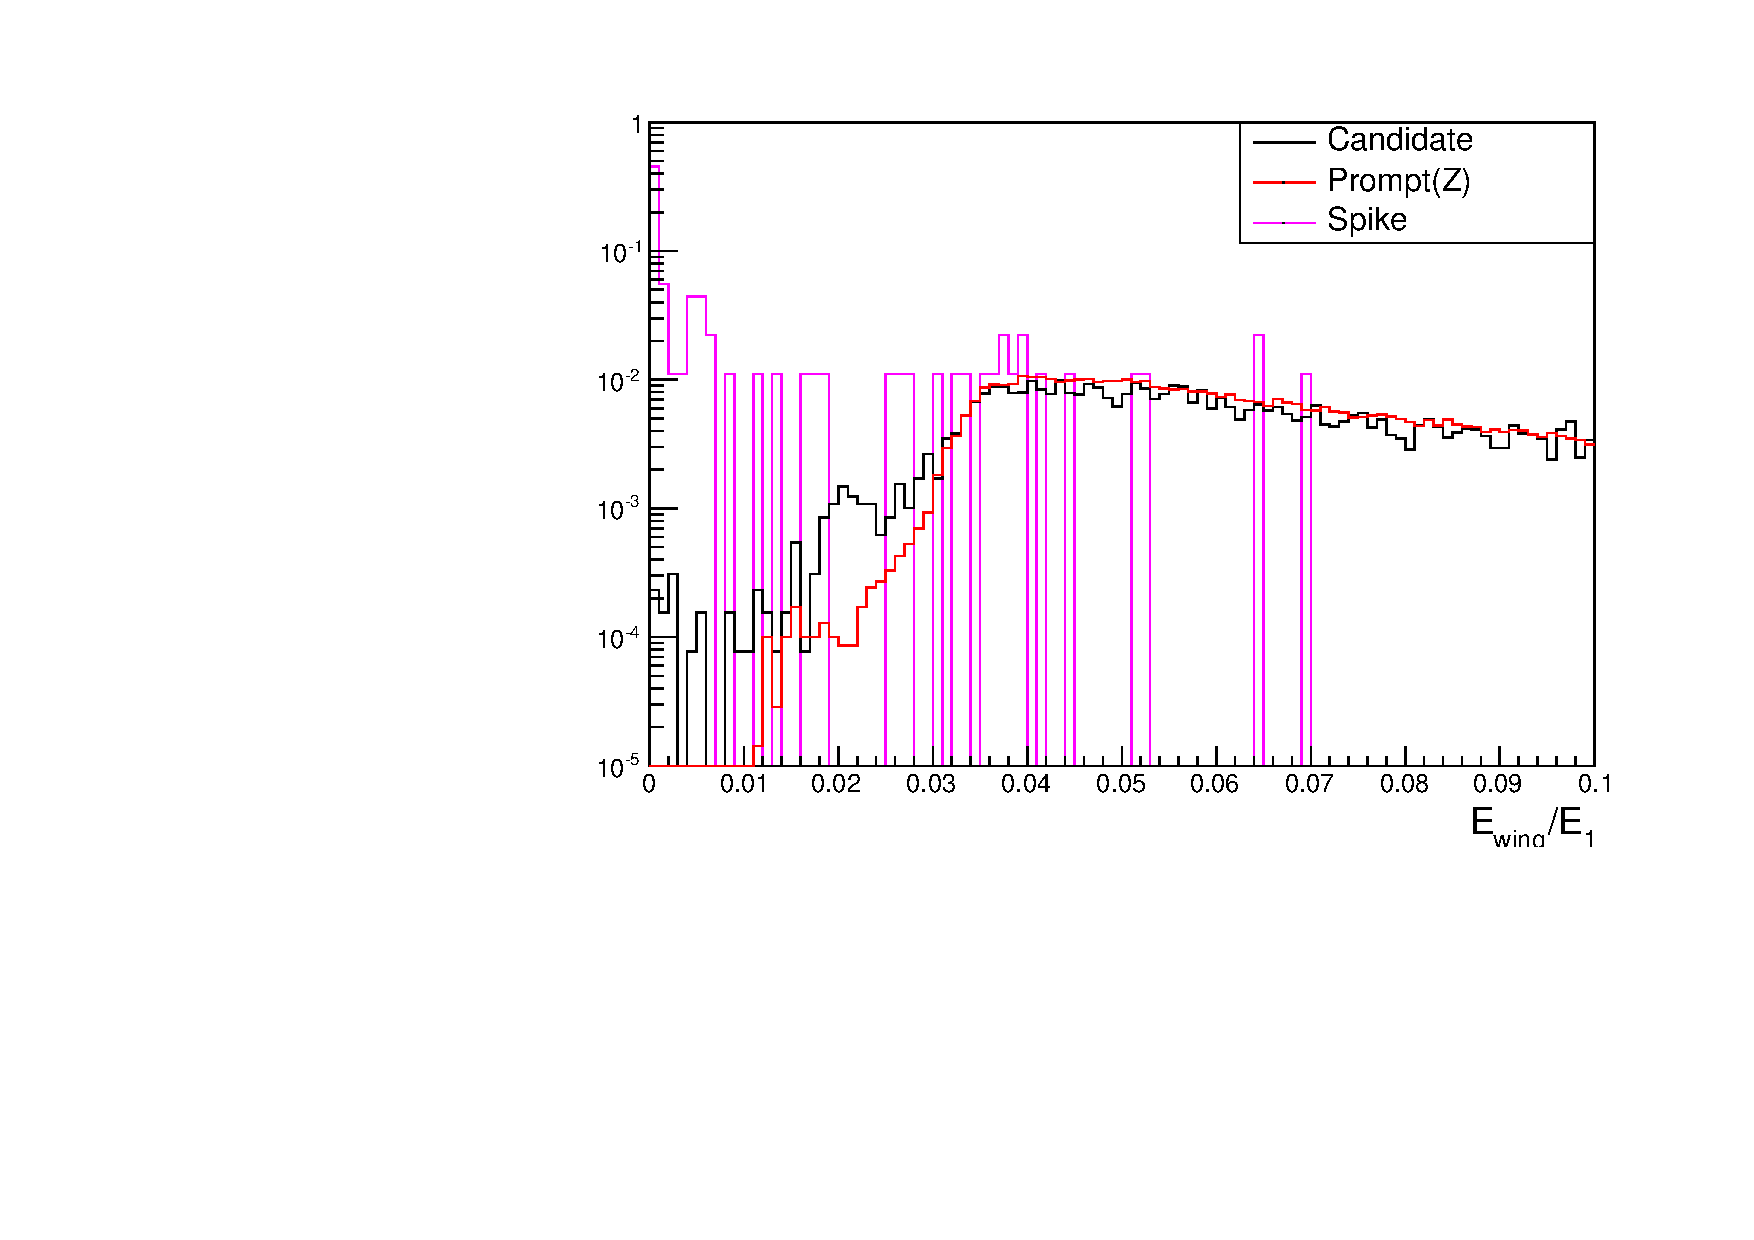
\includegraphics[width=8cm,height=6.5cm]{Figures/noncol/EtaWingCompZLog.pdf}
    \caption{$W_{\eta}$ distribution for electron and spike candidates.}
    \label{fig:etawing}
  \end{center}
\end{figure}

The total number of reconstructed photon candidates can be written as
\begin{equation}
n_\mathrm{tot} = n_\mathrm{spike} + n_\mathrm{real}
\end{equation}
and the total number passing at cut of $W_{\eta} > 0.01$ can be written as
\begin{equation}
n_\mathrm{cut} = \epsilon_\mathrm{spike} n_\mathrm{spike} + \epsilon_\mathrm{real} n_\mathrm{real}
\end{equation}
where $\epsilon_\mathrm{spike}$ and $\epsilon_\mathrm{real}$ are the selection efficiencies of spike and real candidates, respectively,
under the cut. Combining the equations to eliminate $n_\mathrm{real}$ and solving for $n_\mathrm{spike}$ gives
\begin{equation}
n_\mathrm{spike} = (\epsilon_\mathrm{real} n_\mathrm{tot} - n_\mathrm{cut}) / (\epsilon_\mathrm{real} - \epsilon_\mathrm{spike})
\end{equation}
These algebraic manipulations can be expressed as a problem of matrix inversion, and so this method is called the \textit{matrix method}.

The efficiency $\epsilon_\mathrm{spike}$ was measured in a spike control sample (defined by $\sieie < 0.001$ or $\sipip < 0.001$) to be 34.4\%,
and the efficiency $\epsilon_\mathrm{real}$ was measured $\PZ\rightarrow\Pe\Pe$ sample to be 99.9\%.
A total of 12887 events pass a loosened photon ID like the one described above, and out of those, 12872 pass the cut $W_{\eta} > 0.01$, yielding
a total estimated spike yield of $22.9 \pm 6.2$ events, in which the uncertainty is statistical. This is compatible with the total estimated spike yield of
23.9 events obtained from integrating the timing template fit, and provides a cross-check of that method.
In this thesis, the timing template fit
estimate is used as the final estimated spike yield, and the relative uncertainty on the spike yield is taken to be the sum in quadrature of the
20\% uncertainty from the template fit and the 27\% uncertainty from the matrix method estimate, giving a total relative uncertainty of 33\%.

\section{\texorpdfstring{\zinvg}{Z plus gamma} unfolding}
A \zinvg\ event may or may not pass the signal region cuts; if it passes, it will be recorded in a specific \ETgamma\ bin.
For a \zinvg\ event produced with some true \pTgamma\ value within a given \pTgamma\ bin, the probability that
the event will both pass the signal region cuts and subsequently fall in a given reconstructed \ETgamma\ bin is estimated
using MadGraph MC, with higher-order corrections applied.
The $6{\times}6$ matrix of all such probabilities is called the \zinvg\ response matrix, illustrated in Fig.~\ref{fig:response_matrix}.
Its values are listed in Table~\ref{tab:response_matrix_values}.

\begin{figure}[htbp]
  \centering
  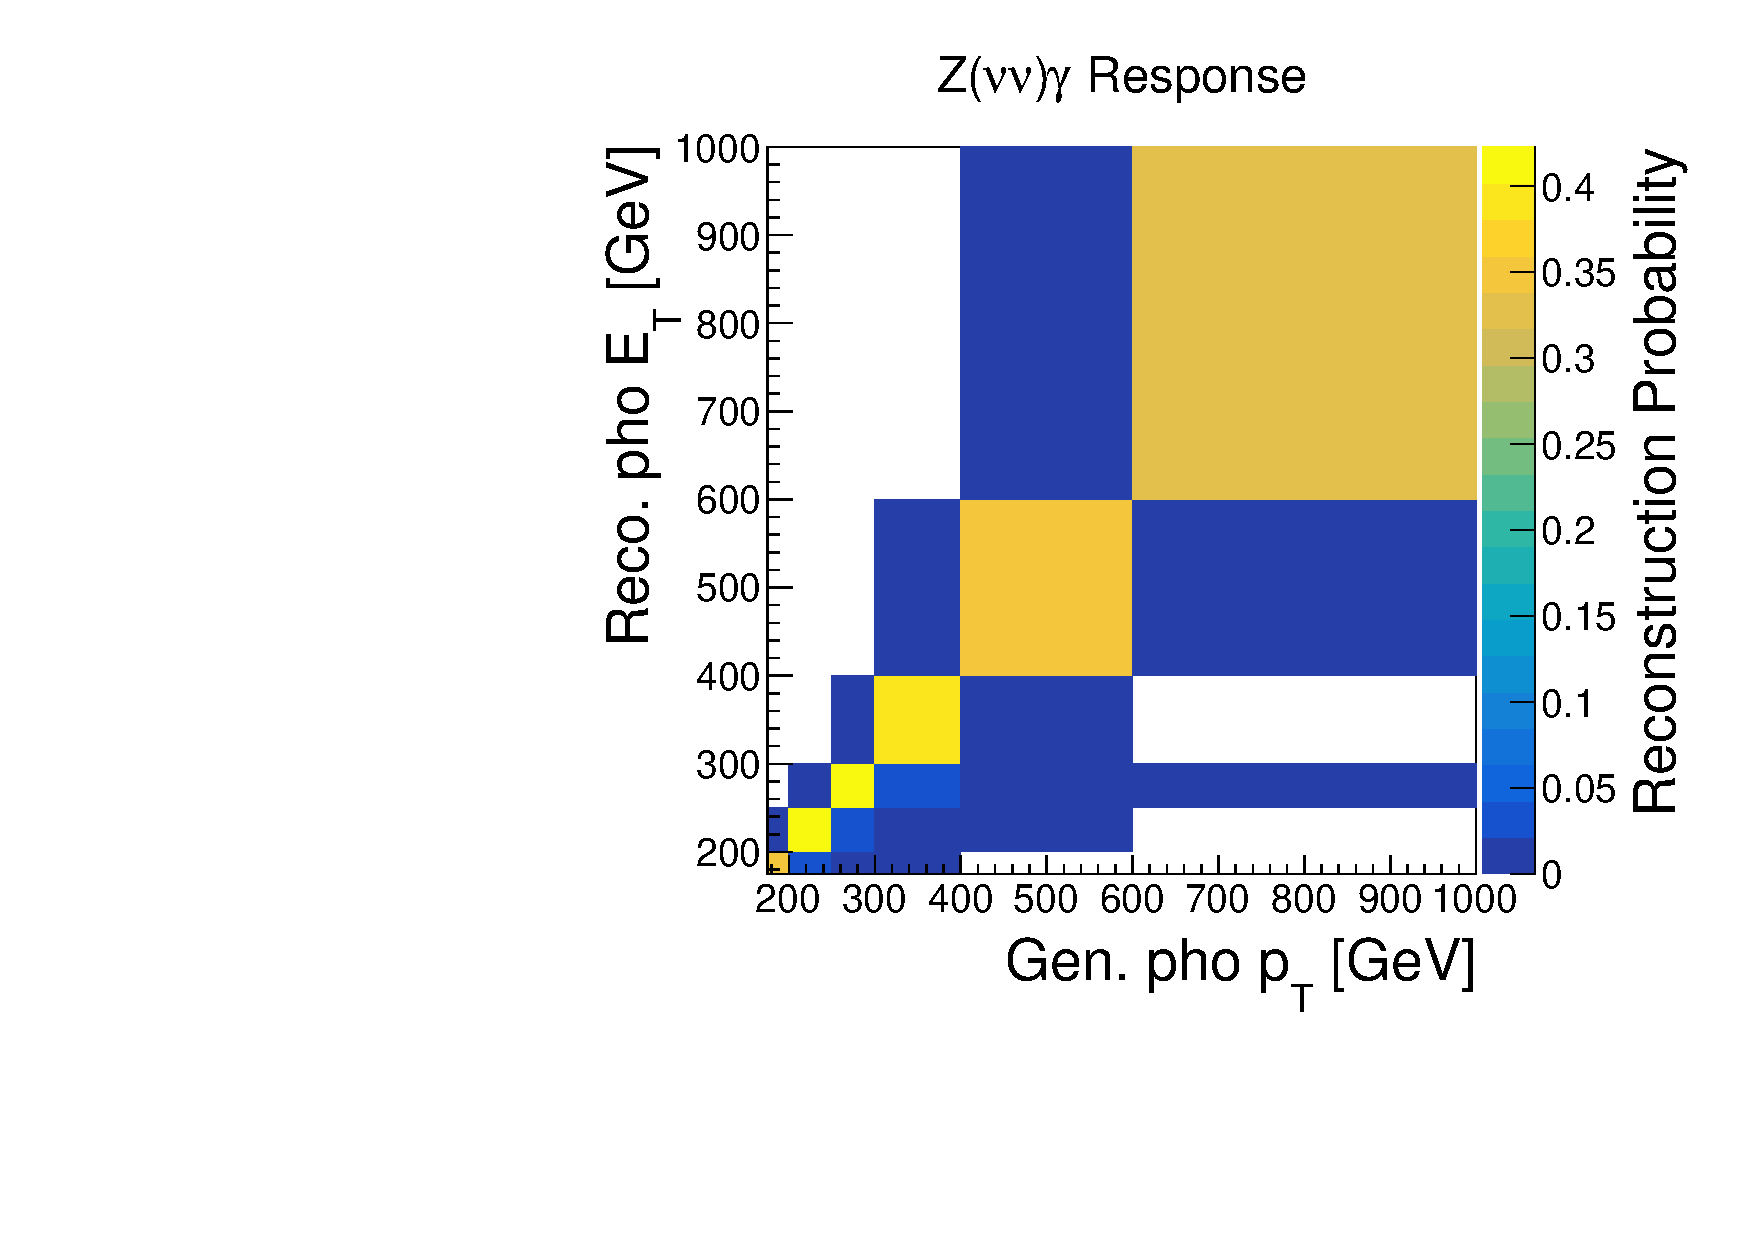
\includegraphics[width=0.6\linewidth]{Figures/znng_response_matrix.pdf}
  \caption{Graphical illustration of the \zinvg\ response matrix. For comparison with Table~\ref{tab:response_matrix_values},
  order the rows from bottom to top and the columns from left to right.}
  \label{fig:response_matrix}
\end{figure}

\begin{table}[tbp]
  \begin{center}
    \caption{
      The values of the response matrix $K$, estimated in \zinvg\ MadGraph MC with higher order corrections applied.
      With rows ordered from top to bottom and columns ordered from left to right, the value in row $i$, column $j$
      is equal to the conditional probability of a \zinvg\ event to pass all signal region cuts and land in reconstructed
      \ETgamma\ bin $j$, if its true \pTgamma\ value is in bin $i$.
    }
    \label{tab:response_matrix_values}
    \begin{tabular}{c c c c c c}
      \hline
       0.297401 & 0.0428149 & 0.000595967 & 5.87982e-05 & 0 & 0 \\
       0.0399934 & 0.38611 & 0.049973 & 0.000505446 & 0.000133614 & 0 \\
       0.000202488 & 0.0214437 & 0.37027 & 0.0326231 & 0.000264926 & 0.000183209 \\
       0 & 0.000196144 & 0.0229108 & 0.367465 & 0.0249473 & 0 \\
       0 & 0 & 1.50756e-05 & 0.0100609 & 0.343767 & 0.022748 \\
       0 & 0 & 0 & 0 & 0.00326465 & 0.316482 \\
      \hline
    \end{tabular}
  \end{center}
\end{table}

Measuring the \zinvg\ differential cross section amounts to extracting the true number of \zinvg\ events in each bin of \pTgamma, and
dividing by the integrated luminosity of our dataset. We denote the total numbers of events expected in each of our six reconstructed
\ETgamma\ bins by a vector $N$, and the expected background (anything other than \zinvg) by a vector $b$. The numbers
of produced \zinvg\ events, represented by $\lambda$, are related to $N$ and $b$ by the expected response matrix $K$ according to
\begin{equation}
  N = K \lambda + b.
\end{equation}
The problem of extracting the differential \zinvg\ cross section from the observed \ETgamma\ distribution---unfolding---is then essentially a problem
of matrix inversion, in which we want to find
\begin{equation}
  \lambda = K^{-1} (N - b).
\end{equation}

To perform the unfolding, we start by assuming that $K$ is equal to the
matrix we estimate in MC (with some systematic uncertainties), and then we find the values of the vector $\lambda$ that result in the greatest
compatibility between $K \lambda + b$ and the observed number of signal region events. Taking ``greatest compatibility'' to mean an ML
estimate, this is equivalent to the problem of matrix inversion
stated above, with $K$ and $b$ set to their best-fit values and $N$ set to the observed number of signal region events.

The response matrix $K$ is close to diagonal, which indicates that a \zinvg\ photon with a given true value of \pTgamma\ is usually measured
to have a similar reconstructed value of \ETgamma\ (i.e. within the same \ETgamma\ bin),
as long as the \zinvg\ event first passes all signal region cuts. Nevertheless, some \zinvg\ events do have reconstructed \ETgamma\ values
in bins other than the true \pTgamma\ bin, and so in general, \zinvg\ events from a single true \ETgamma bin will produce
a distribution of reconstructed \ETgamma\ values spread across multiple bins (though concentrated mainly on the true bin).
The shapes of these six distributions correspond to the six columns of $K$. Taking column $i$ of $K$ and multiplying by entry $i$ of $\lambda$ gives
the reconstructed \zinvg\ event yield in the signal regions for photons with true \pTgamma\ in bin $i$; $K \lambda$ is the vector of reconstructed \zinvg\ event yields summed
over all true \pTgamma\ bins.

In the fit, $K \lambda$ is represented by a sum of six reconstructed \ETgamma\ histograms, one for each true \pTgamma\ bin. Each histogram is assigned a single overall
multiplicative scale factor $r_{i}$, which are free parameters of the fit.
Initially, each $r_{i}$ is set to 1.0, and each histogram represents the expected \zinvg\ yield estimated in MC. After the fit, each factor $r_{i}$ represents the factor
by which the initial MC estimate in true \ETgamma\ bin $i$ must be multiplied in order to arrive at the observed best-fit distribution. In other words, the postfit value
of the number of produced events $\lambda_{i}$ is equal to its prefit value times $r_{i}$.
Since the number of produced events is equal, on average, to cross section times luminosity, we conclude that the postfit \zinvg\ cross
section in bin $i$ is equal to the prefit cross section from MC multiplied by the postfit value of $r_{i}$.

Because $K$ is strongly diagonal and has similar values all along its diagonal, its inversion is not expected to result in any mathematical pathologies.
The condition number of the matrix, defined to be the ratio of its largest to its smallest singular value, is 1.5363. It is invertible, and
its inversion produces positive estimates of the cross section in every \ETgamma\ bin. There is no clear motivation to employ any sort of regularization
strategy in the ML fit, and we do not employ any such strategy.

For the purposes of this section, a \zinvg\ event is only considered to
have been produced in a given true \pTgamma\ bin if the photon additionally falls within the barrel acceptance ($|\eta| < 1.4442$) and
if the vector sum of the transverse momenta of the two neutrinos has a magnitude greater than 170\unit{GeV}. A \zinvg\ event failing one of these
criteria, or with \ETgamma\ less than 175 GeV, is considered to be a source of background. The expected contribution of these background events is estimated
purely in MC.

\section{Higher-order corrections}
The largest expected SM contributions to the various signal and control regions are from three $\mathrm{V}\gamma$
processes: \zinvg, \wlng, and \zllg.
The \zinvg\ response matrix (for the cross section measurement), the SM \zinvg\ yield (for aTGC limits),
and \wlng\ and \zllg\ transfer factors (described in the next section) are modeled using MC simulations.
As with other signal and background processes estimated in MC, these samples are generated to LO in QCD by MadGraph.
These $\mathrm{V}\gamma$ processes are generated with up to two extra gluons radiated from the incoming quarks,
which form jets in the final detected event.
For the aTGC analysis, redundant \zinvg\ samples are generated to LO in QCD by Sherpa, with no additional jets.

To approximate higher-order QCD effects, \zinvg\ and \wlng\ events are reweighted based on \pTgamma\ by the factors
given in Tab.~\ref{tab:zg_kfactors}. These factors are the ratios of NNLO differential cross sections calculated by
Grazzini et al.~\cite{ref:j.physletb.2010.12.024} to the cross sections of the LO MC samples described above\footnote{Since the LO samples include
contributions from processes with up to two additional radiated particles, they are therefore not LO in the strictest sense.
$\mathrm{V}\gamma$ k-factors found in the literature can be much larger than 1.0 at high \pTgamma,
if the denominator only accounts for the cross section of the $\Pq\Paq\rightarrow\mathrm{V}\gamma$ process with no additional parton
radiation.}. The renormalization and factorization scale uncertainties on the NNLO cross section correction factors range from 7 to 8\%,
depending on the \pTgamma\ bin. These uncertainties are assessed by varying the respective scales by factors of 2 and 0.5 during
the cross section computation.

\begin{table}
  \begin{center}
    \caption{NNLO / LO correction factors for \zinvg\ and \wlng\ samples.}
    \label{tab:zg_kfactors}
    \begin{tabular}{| l | r | r |}
      \hline
      \pTgamma\ [GeV] & \zinvg & \wlng \\
      \hline
      \hline
      $[175, 190]$ & 1.44 & 1.40 \\
      \hline
      $[190, 250]$ & 1.41 & 1.37 \\
      \hline
      $[250, 400]$ & 1.35 & 1.31 \\
      \hline
      $[400, 700]$ & 1.29 & 1.26 \\
      \hline
      $[700, \inf]$ & 1.15 & 1.15 \\
      \hline
    \end{tabular}
  \end{center}
\end{table}

Out of various higher-order electroweak effects, ones that can give sizeable
($\gg\mathcal{O}(\alpha)$) corrections to the cross section are Sudakov suppression at high boson \pT\ and
potentially the addition of photon-induced scattering
processes~\cite{ref:JHEP04(2015)018, ref:JHEP02(2016)057}. The correction factors shown in
Figure~\ref{fig:ewk_correction} are combinations of Sudakov suppression factors and
photon-induced enhancements computed by the authors of Ref.~\cite{ref:JHEP02(2016)057}. These are applied to the $\mathrm{V}\gamma$
samples on top of the NNLO QCD correction factors, as a function of \pTgamma.

\begin{figure}[htbp]
  \centering
  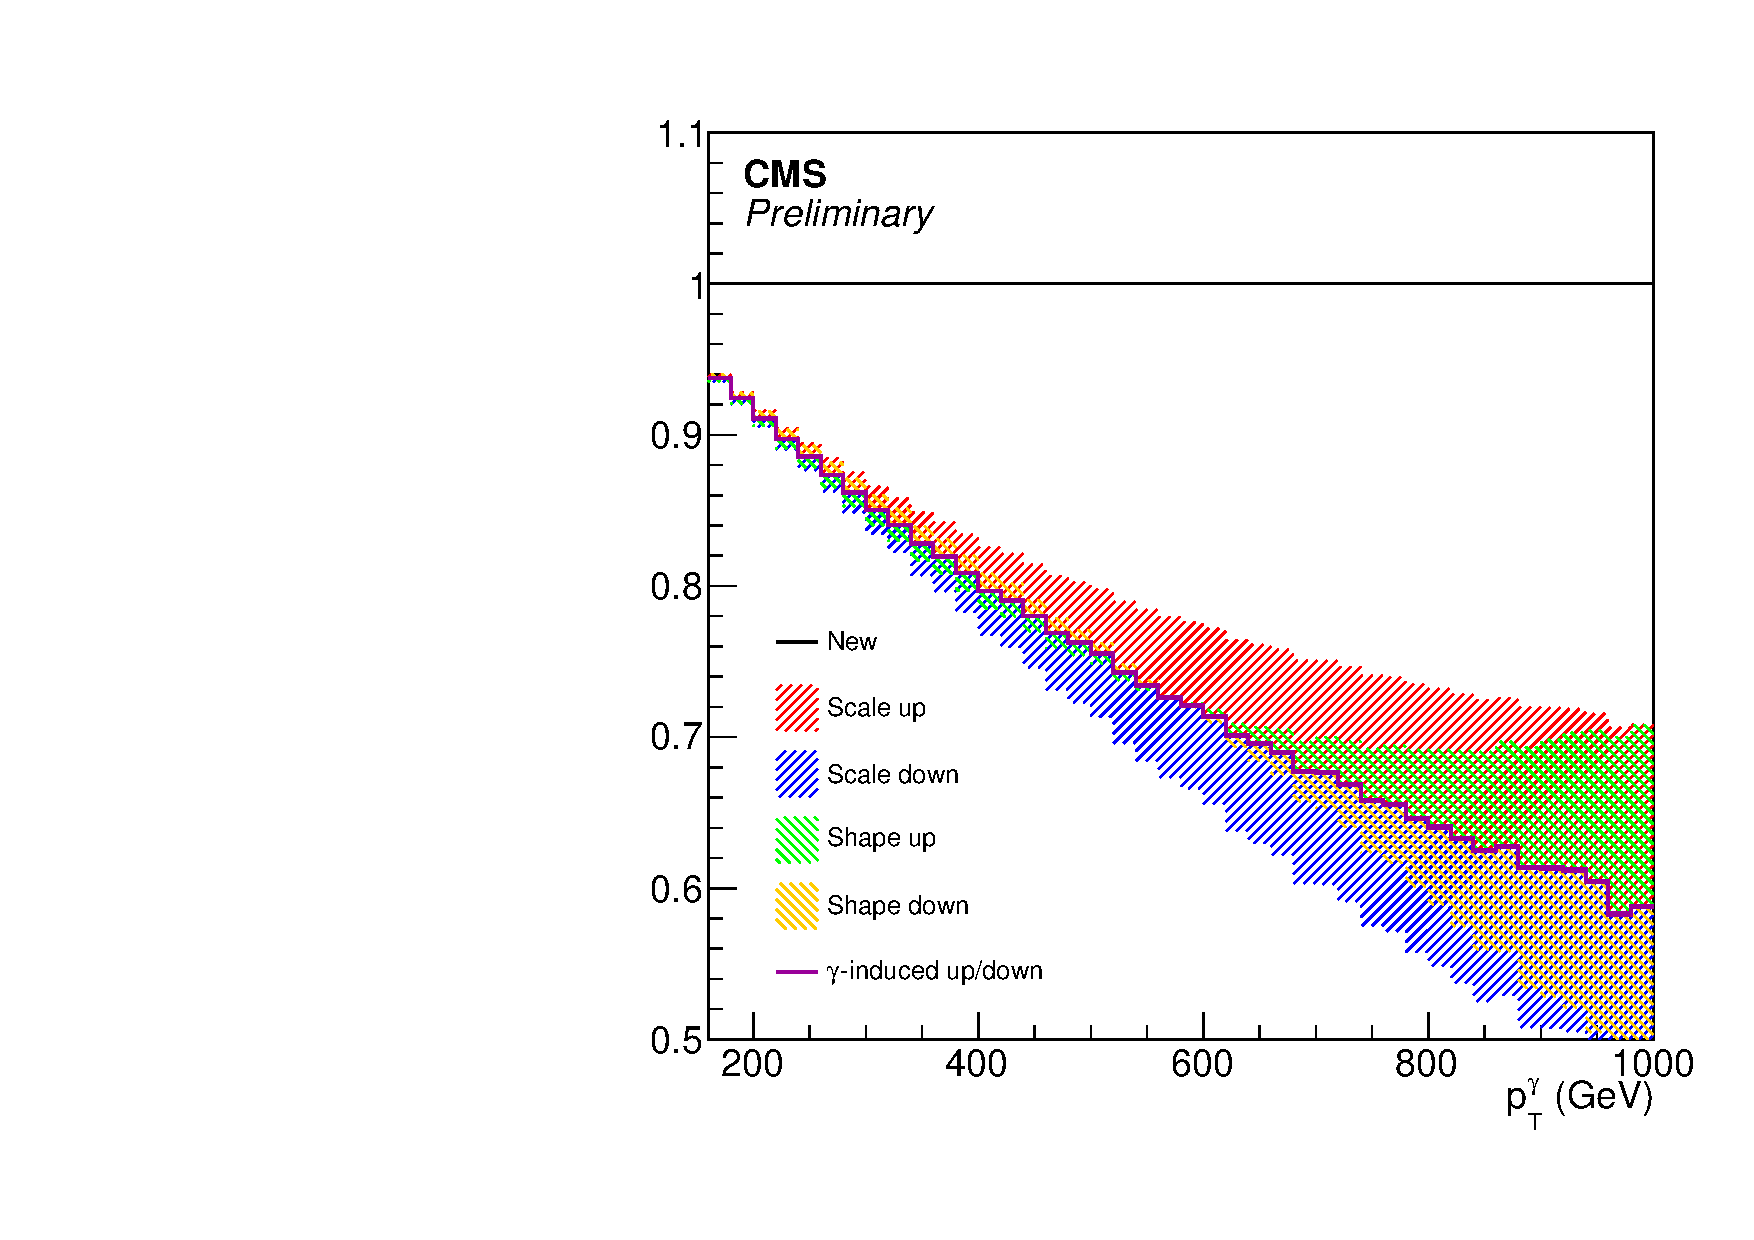
\includegraphics[width=0.4\linewidth]{Figures/vg/ewk_zg.pdf}
  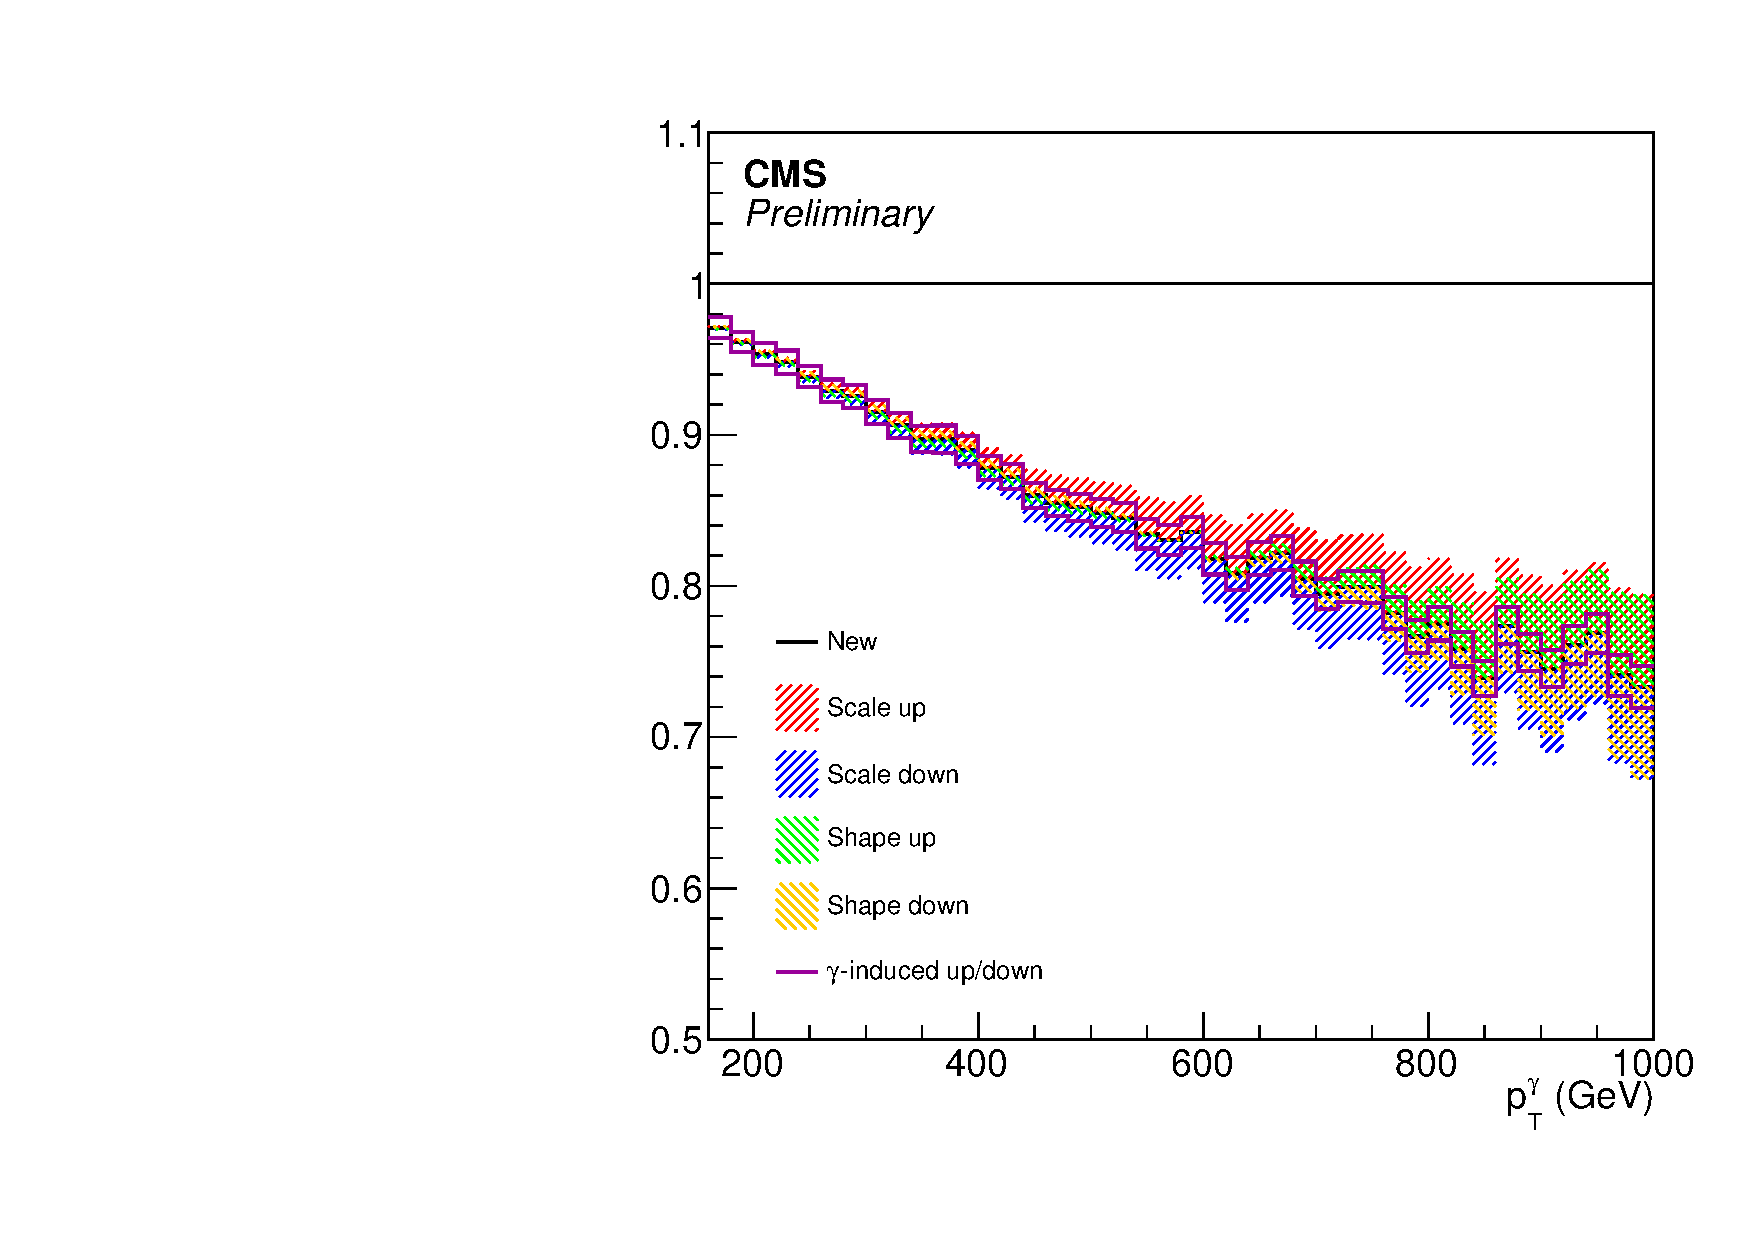
\includegraphics[width=0.4\linewidth]{Figures/vg/ewk_wpg.pdf}
  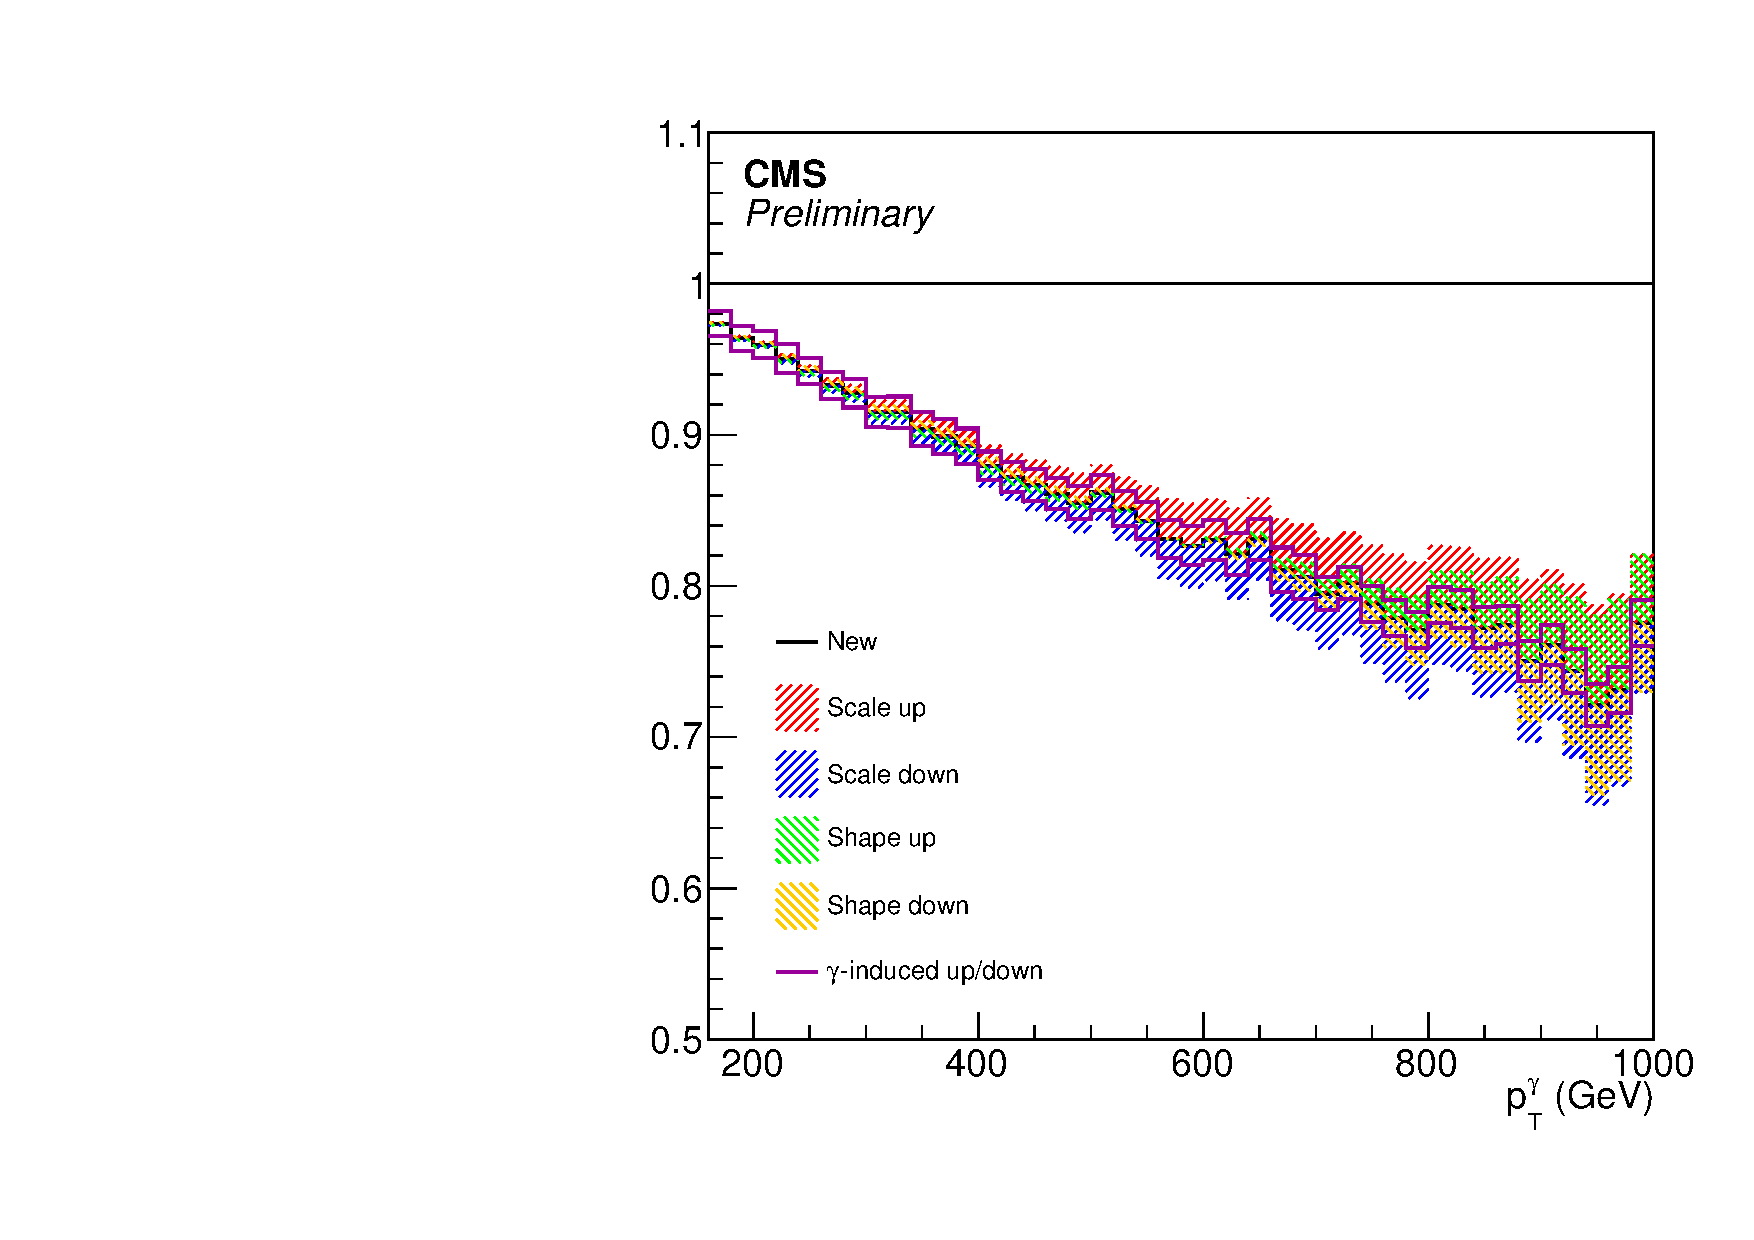
\includegraphics[width=0.4\linewidth]{Figures/vg/ewk_wmg.pdf}
  \caption{
    Electroweak NLO cross section corrections as a function of \pTgamma\ for $\PZ{+}\Pgamma$, $\PWplus{+}\Pgamma$, and $\PWminus{+}\Pgamma$
    processes, overlaid with uncertainty bands.
  }
  \label{fig:ewk_correction}
\end{figure}

The differential cross section after all higher-order corrections are applied may be written as
\begin{equation}
  d\sigma^{\mathrm{NNLO QCD}+\mathrm{NLO EWK}} = d\sigma^{\mathrm{LO}} k^{\mathrm{NNLO QCD}} (1 + \kappa^{\mathrm{EWK Sudakov}} + \kappa^{\mathrm{EWK} \Pq\Pgamma}),
\end{equation}
where $k^{\mathrm{NNLO QCD}} = d\sigma^{\mathrm{NNLO QCD}} / d\sigma^{\mathrm{LO}}$, and the two $\kappa$
terms are the Sudakov suppression and photon-induced enhancement components of the EWK
correction, respectively.

Theoretical uncertainties on the EWK corrections are not currently well-understood. In this thesis,
the magnitudes of the uncertainties on $\kappa^{\mathrm{EWK Sudakov}}$ and $\kappa^{\mathrm{EWK} \Pq\Pgamma}$ are estimated
to be $(\kappa^{\mathrm{EWK Sudakov}})^2$ and $\kappa^{\mathrm{EWK} \Pq\Pgamma}$, i.e. the square of
the correction and 100\% of the correction, respectively\footnote{Choosing the square of $\kappa^{\mathrm{EWK Sudakov}}$ is motivated by the fact
that fully resummed leading-log Sudakov suppression is an exponential function of $\kappa^{\mathrm{EWK Sudakov}}$.}.

For the Sudakov suppression, which is the dominant term in the EWK correction, we further
consider two types of systematic variations, inspired by ref.~\cite{ref:epjc/s10052-017-5389-1}, which provides
a prescription for EWK correction uncertainties for $\mathrm{V}+\mathrm{jets}$ processes. In
this thesis, the EWK correction as a function of \pTgamma\ is varied in overall scale and in
slope. The two types of variation have maximum magnitudes such that their sum, in quadrature, equals the full
magnitude of the estimated Sudakov uncertainty. The slope variation is obtained by selecting a point in the \pTgamma\ spectrum and forcing
the shift in the correction to cross over at that point (see Figure~\ref{fig:ewk_correction_cartoon}). The specific crossover
point chosen in this thesis is $\pTgamma = 590\unit{GeV}$. Final results do not strongly depend on the
specific choice of crossover point.

\begin{figure}[htbp]
  \centering
  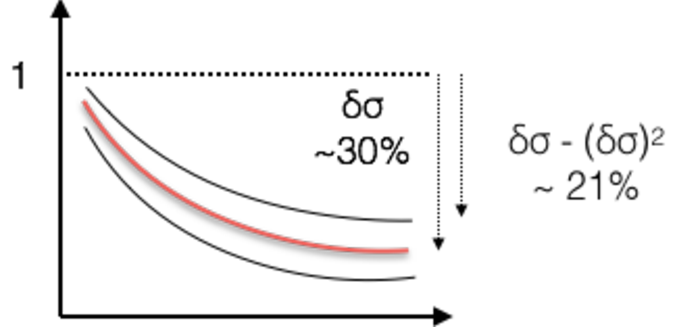
\includegraphics[height=0.3\linewidth]{Figures/vg/ewk_correction_scale.pdf}
  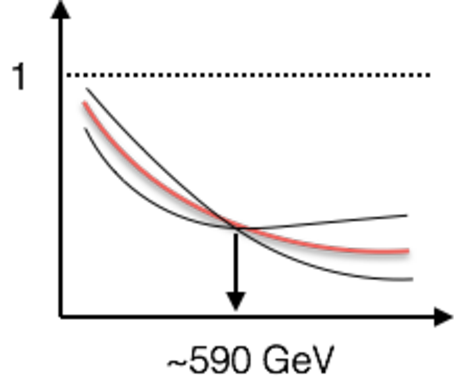
\includegraphics[height=0.3\linewidth]{Figures/vg/ewk_correction_shape.pdf}
  \caption{
    Electroweak correction variation scheme to cover the scale (left) and shape (right) uncertainties.
  }
  \label{fig:ewk_correction_cartoon}
\end{figure}

\section{Signal estimation: SM and aTGC} \label{sec:signal_extraction_SM_aTGC}
Beam halo is the only process examined in this analysis with an anisotropic $\phi$ distribution.
Figure~\ref{fig:halophi} shows the distribution of beam halo photons as a function of $\phi'$.
To constrain the beam halo normalization, the signal region is split into two parts according to $|\phi'|$.
The parts defined by $|\phi'| < 0.5$ and $|\phi'| > 0.5$ are respectively called the horizontal ($H$) and vertical ($V$) signal
regions. All other sources of events have expected yields that are isotropic in $\phi$, and therefore
are expected to fall into the two signal regions in direct proportion to the $\phi$ coverage of those regions.
The fraction of the total $\phi$ span covered by signal region $S$ is denoted by $C_{S}$ ($S \in \{H,V\}$).

\begin{figure}[tbp]
  \begin{center}
    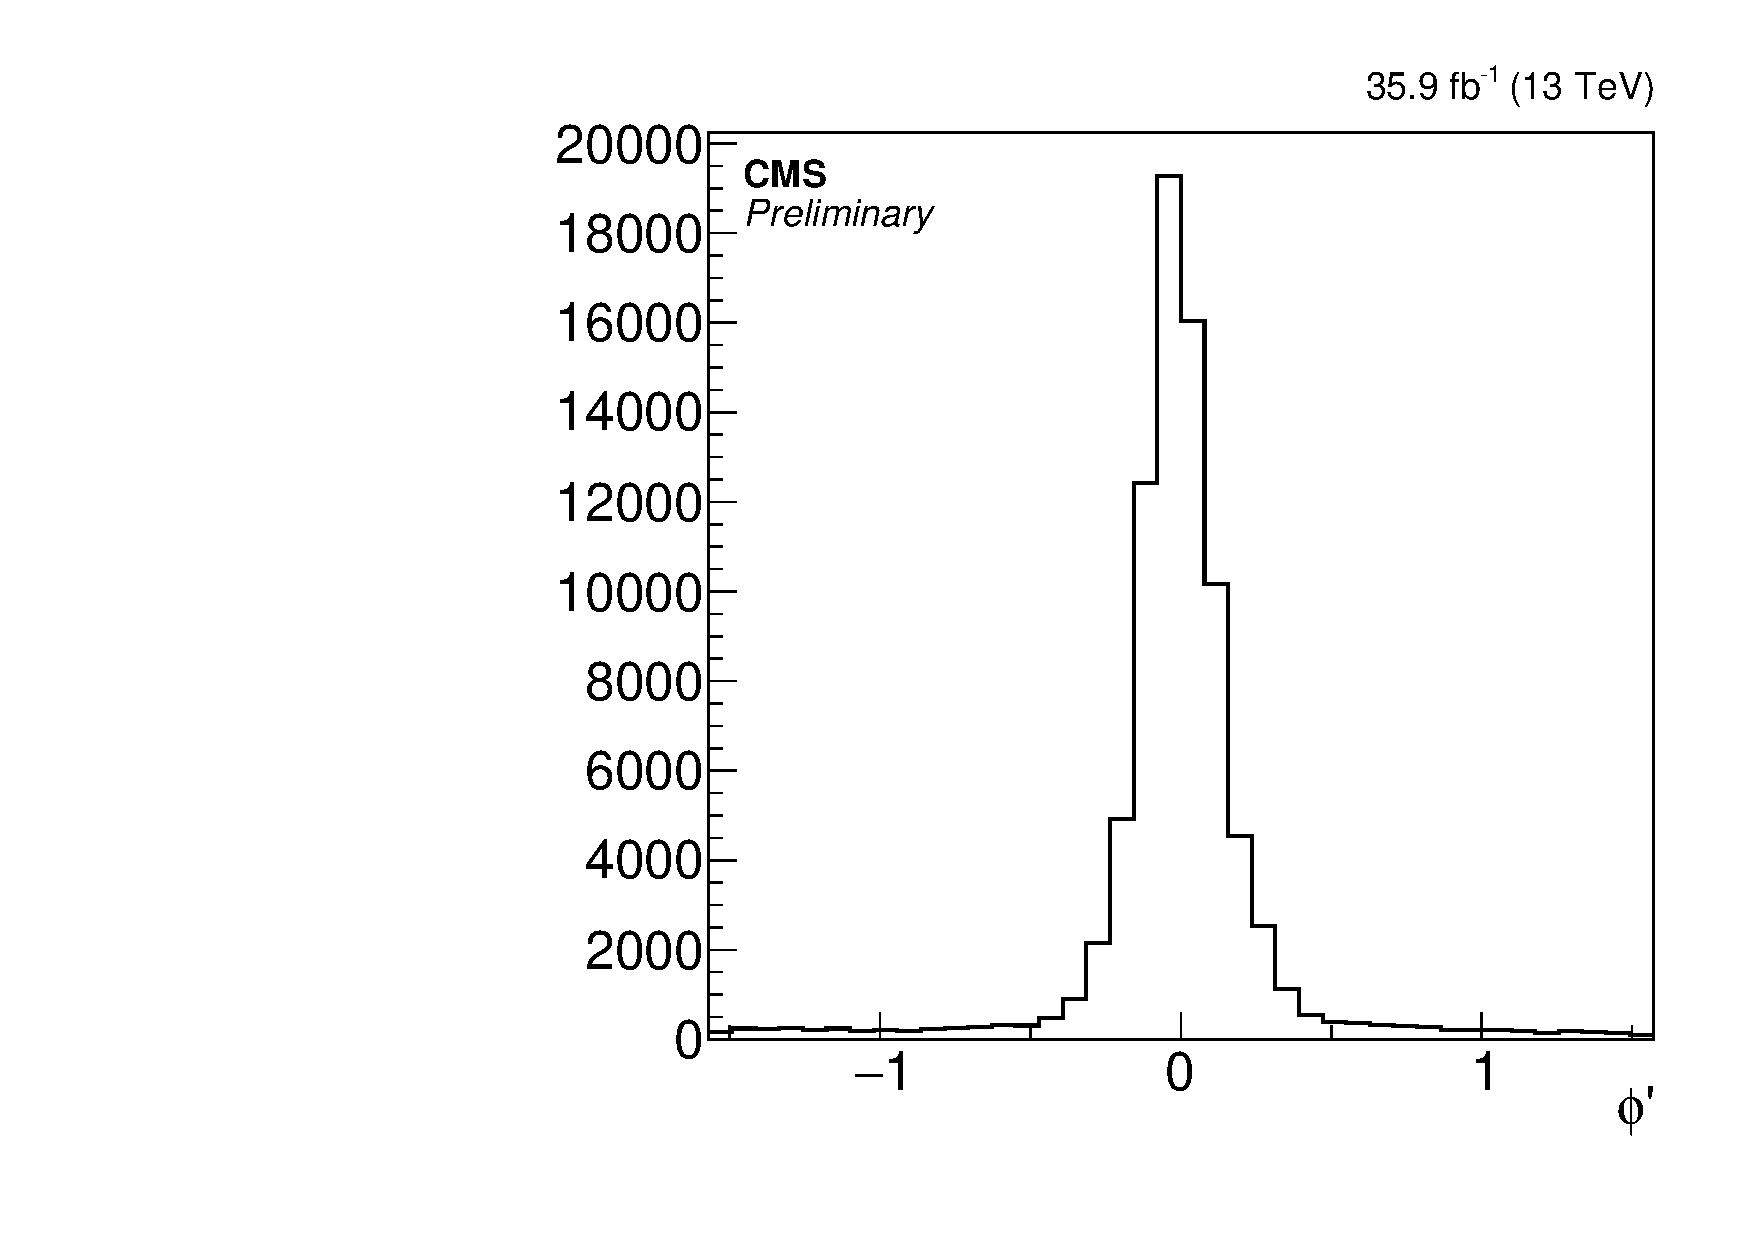
\includegraphics[width=0.45\textwidth]{figures/noncol/phiHaloFolded.pdf}
    \caption{
      $\phi'$ distribution of beam halo photons in observed events with $\MET > 170\unit{GeV}$. A reconstructed photon is included
      in this plot if it fails one of the beam halo \MET\ filters and has $\ETgamma > 175\unit{GeV}$ and
      $\mathrm{MIP total energy}>4.9\unit{GeV}$.
    }
    \label{fig:halophi}
  \end{center}
\end{figure}

The fraction of beam halo events in each signal region is determined by comparing the integral of Fig.~\ref{fig:halophi} in the regions
$|\phi'| < 0.5$ and $|\phi'| > 0.5$. The \ETgamma\ dependence of the halo background is estimated in data
by inverting the MIP total energy veto, but requiring all other signal region cuts to be passed. These pieces of information are encoded in 
\nhalo[,j], the estimated beam halo prediction in reco. bin $j$ of the signal region $S$. This is multiplied by a
single parameter $h$ in the fit, which governs the overall normalization of the beam halo yield.

The overall normalization of \zinvg\ from each gen. \pTgamma\ bin $i$ is scaled by a factor $r_{i}$, defined so that
the postfit cross section of gen bin i is equal to the prefit cross section times $r_{i}$.
Each gen \pTgamma\ bin makes contributions to multiple reco \ETgamma\ bins.
The prefit contributions from each gen bin $i$ to each reco bin $j$ (in both signal regions combined) are estimated in MC, and denoted by \nZg[j,i].

Using the above definitions for $C_{S}$, $r_{i}$, $\nZg[j,i]$, $h$, and $\nhalo[,j]$,
the total reconstructed event yield \nS\ in each signal region (excluding aTGC contributions) is estimated according to
\begin{equation}
  \nS[,j] = C_{S} (\Sigma_{i}r_{i}\nZg[j,i] + \nWg[j] + b_{j}) + h\nhalo[,j],
\end{equation}
where $\nWg[j]$ is the total contribution of \wlng\ events to reco bin $j$, and $b_{j}$ is the total contribution to reco bin $j$ from
electron and hadron misidentification, ECAL spikes, and other minor SM background processes, in both signal regions combined.

The ratios (\textit{transfer factors}) of the bin-by-bin yields of \wlng\ in the signal regions to those
of \wlng\ in the single-lepton control regions are denoted by \RWl[,j]. These are estimated in MC.
The total reconstructed event yield \nl\ in each single-$\ell$ control region ($\ell \in \{e,\mu\}$) is estimated according to
\begin{equation}
  \nl[,j] = \frac{\nWg[j]}{\RWl[,j]} + b_{\ell\Pgamma,j},
\end{equation}
where \nWg\ is the number of \wlng\ events in the combined signal regions, and
$b_{\ell\Pgamma}$ is the predicted contribution from other background sources in the single-$l$ control region.
Figure~\ref{fig:tf_w} shows the transfer factors relating the \wlng\ yield in the single-lepton control regions to the \wlng\ yield in the
vertical signal region.

\begin{figure}[htbp]
  \begin{center}
    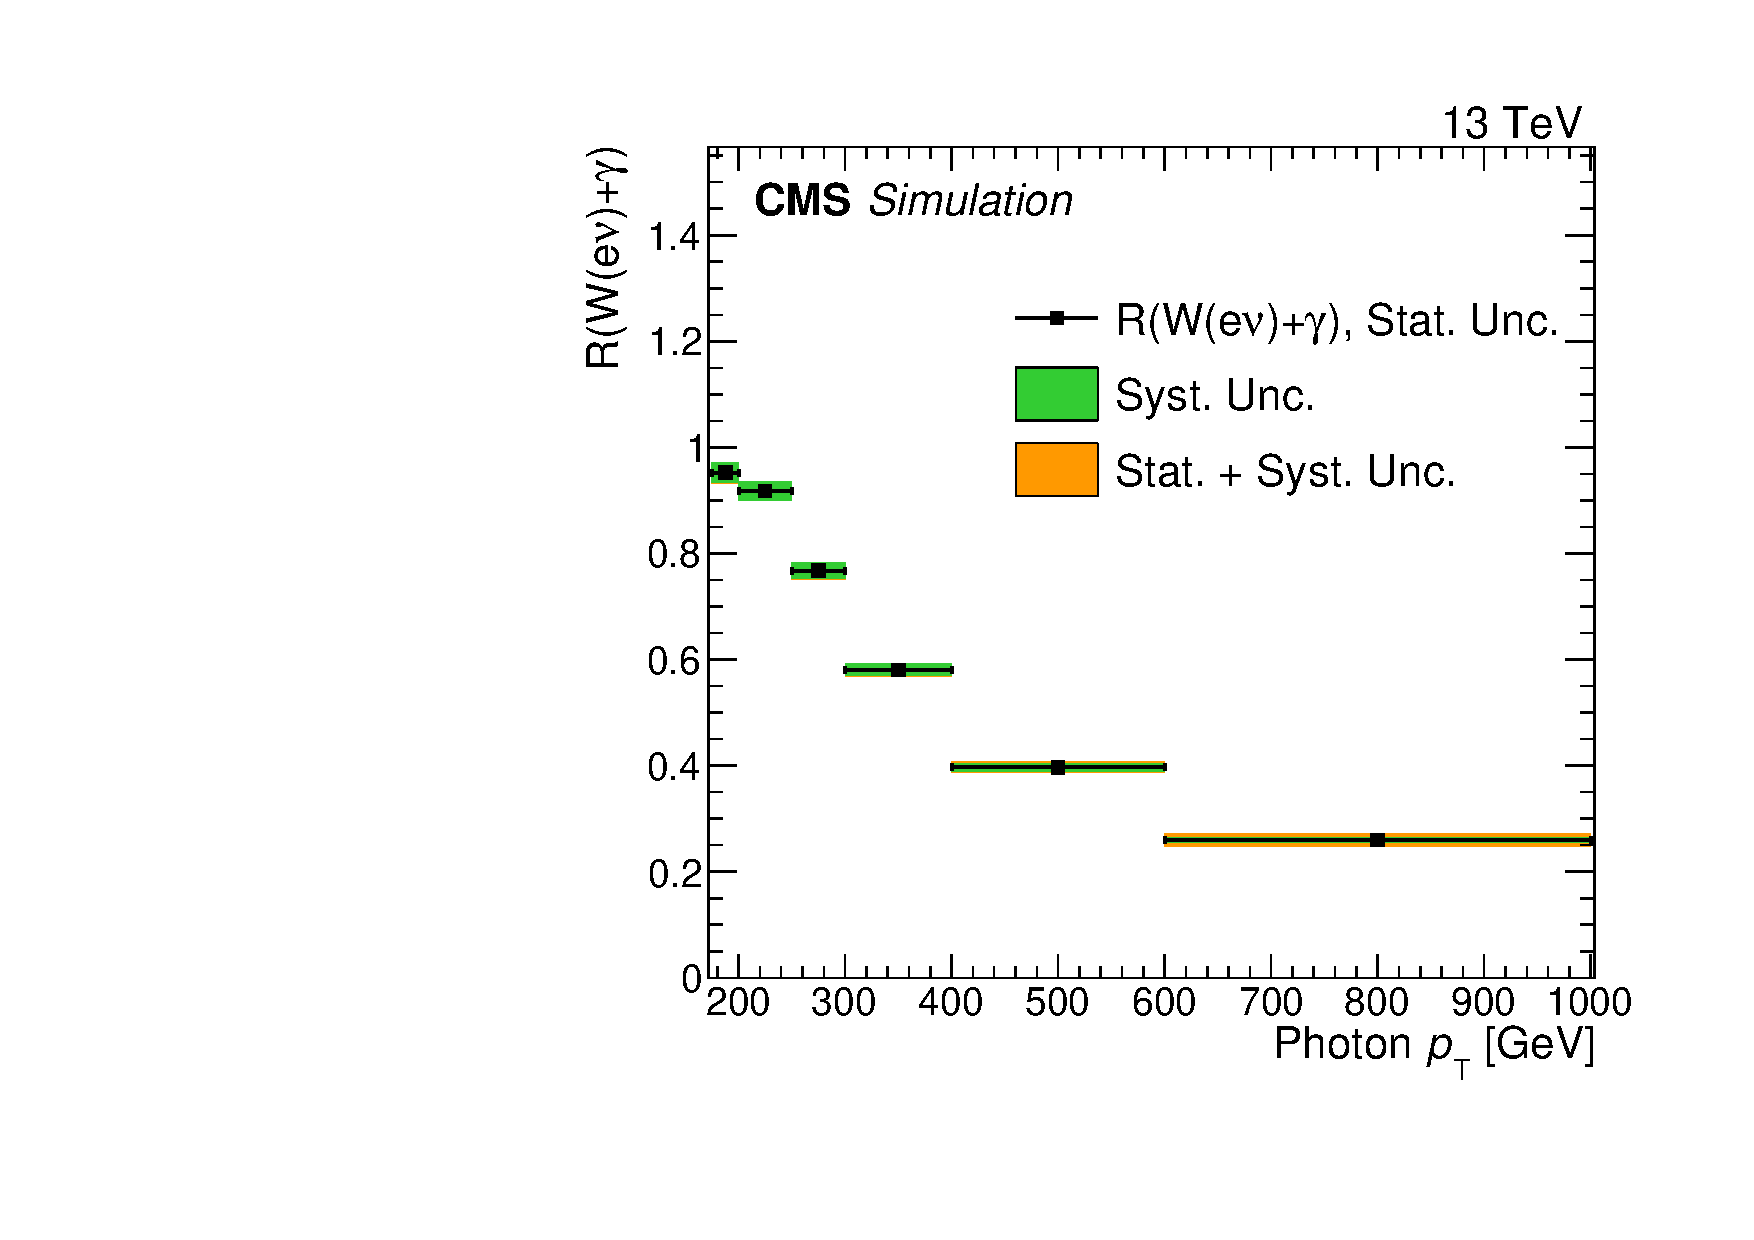
\includegraphics[width=0.45\textwidth]{Figures/results/transfer_WGinZnnG_over_WGinWenG_phoPt.pdf}
    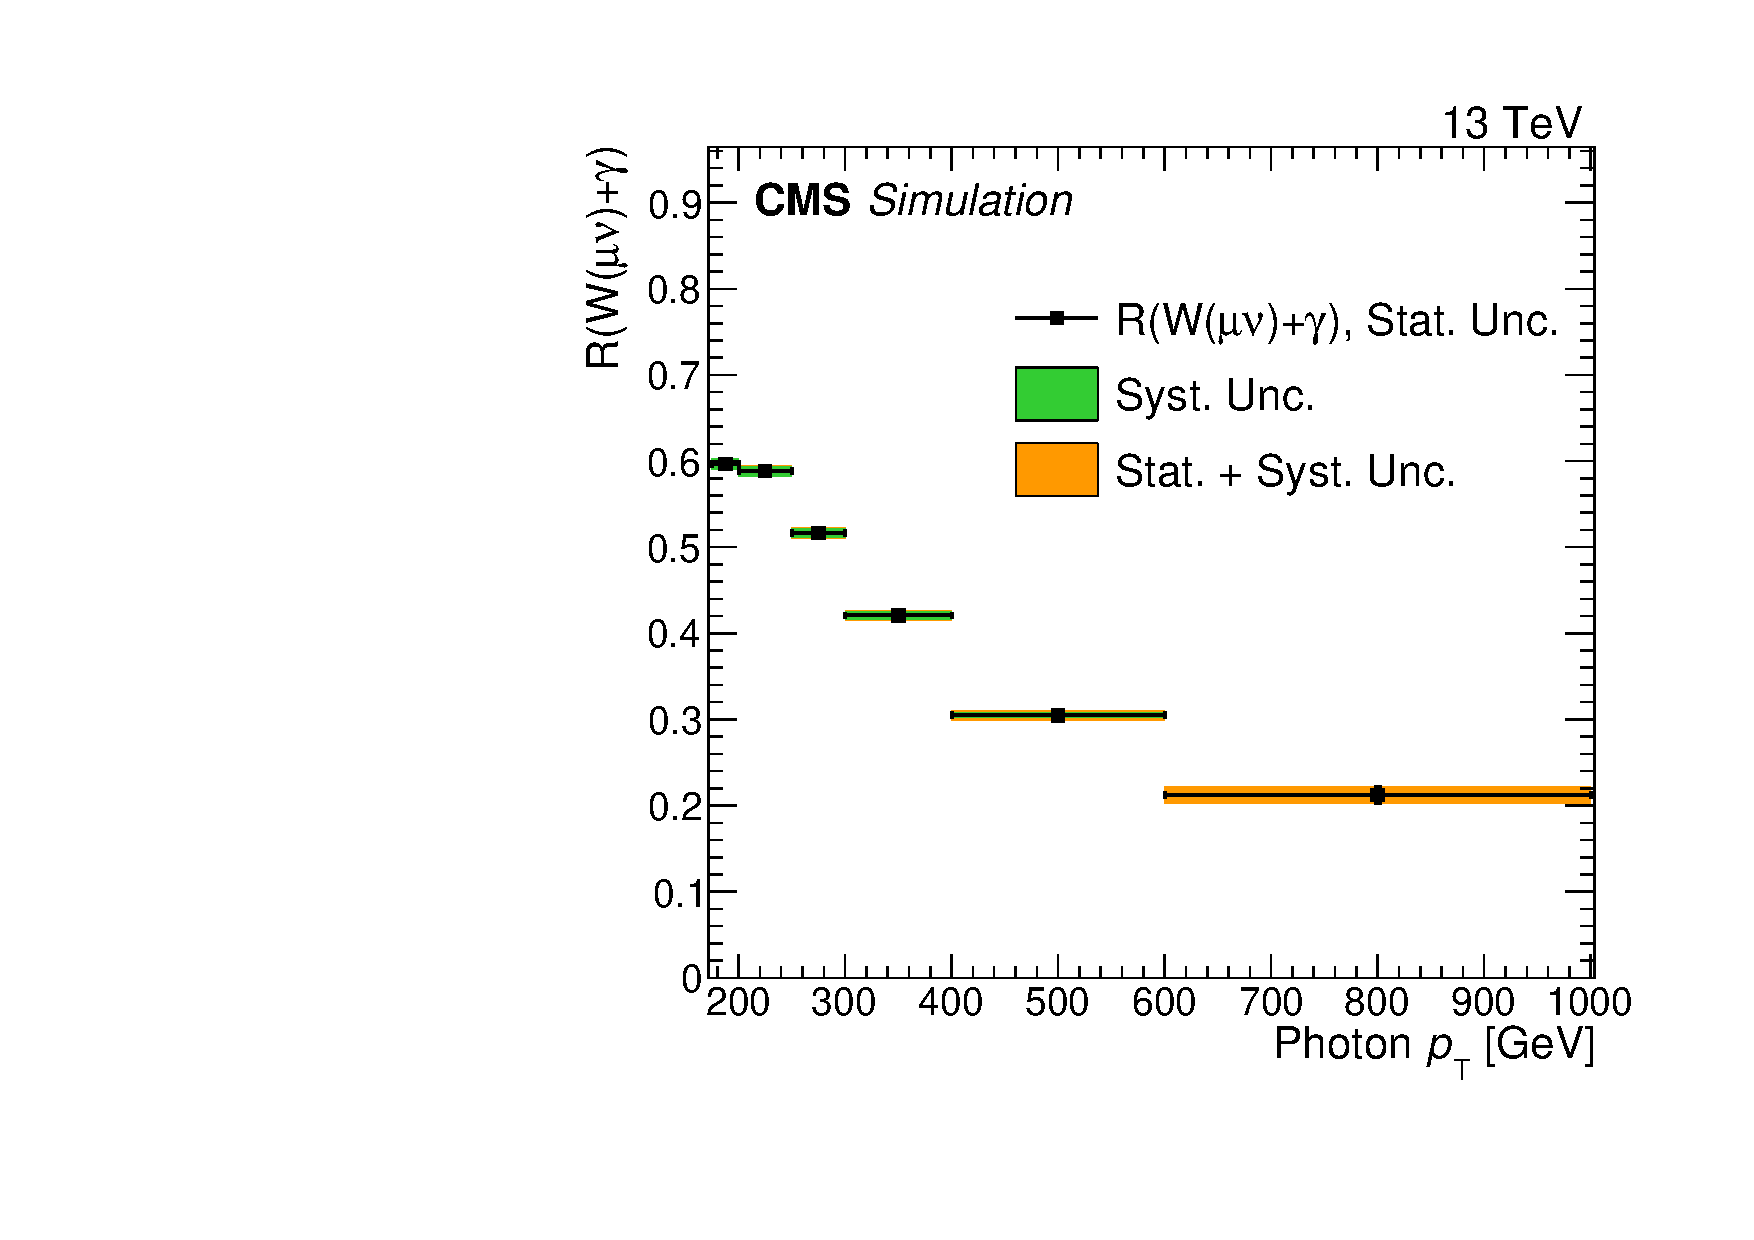
\includegraphics[width=0.45\textwidth]{Figures/results/transfer_WGinZnnG_over_WGinWmnG_phoPt.pdf}
    \caption{
          Transfer factors $R^{\PW\Pgamma}_{\Pe\Pgamma}$ (left) and $R^{\PW\Pgamma}_{\Pmu\Pgamma}$ (right). The last bin includes all events with $\ETgamma > 1000\unit{GeV}$.
    }
    \label{fig:tf_w}
  \end{center}
\end{figure}

The complete likelihood function that is maximized in the SM cross section fit is
\begin{align}
  \mathcal{L} & = \left\{ \mathcal{L_{\text{Signal}}} \mathcal{L_{\text{Control}}} \right\} \times \mathcal{L_{\text{Nuisances}}} \\
  & = \prod_{j} \left\{
    \prod_{S=H,V} \mathcal{P}\left( N_{S, j} \left| \nS[,j] (\vec{\theta} \right.) \right) \prod_{\ell=\Pe,\Pmu} \mathcal{P}\left( N_{\ell\Pgamma, j} \left| \nl[,j] (\vec{\theta}) \right. \right) 
    \right\}  \times \prod_{t} \mathcal{N}(\theta_t) \\
  & = \prod_{j} \left\{
  \begin{array}{cc}
    \prod\limits_{S=H,V} \mathcal{P}\left( N_{S, j} \left| C_{S} \left(\Sigma_{i}r_{i}\nZg[j,i](\vec{\theta}) + \nWg[j] + b_{j}(\vec{\theta})\right) + h \nhalo[,j](\vec{\theta}) \right. \right) \\[1.3pt]
    \times \prod\limits_{\ell=\Pe,\Pmu} \mathcal{P}\left( N_{\ell\Pgamma, j} \left| \frac{\nWg[j]}{\RWl[,j](\vec{\theta})} + b_{\ell\Pgamma, j}(\vec{\theta}) \right. \right) \\[1.3pt]
  \end{array} \right\}
  \times \prod_{t} \mathcal{N}(\theta_t),
\end{align}
following the notation introduced above, and where $\mathcal{P}(N\vert\lambda)$ is the Poisson probability of $N$ for mean $\lambda$,
$\mathcal{N}$ denotes the unit normal distribution centered at zero, and $N_{X,i}$ is the observed number of events in reco bin i of region X.

Systematic uncertainties are handled using nuisance parameters $\theta_{t}$ in the fit.
If a quantity $X$ has a prefit value $\overline{X}$ and if, for every $t$, it has a systematic uncertainty $\sigma_{t}$ corresponding to nuisance
parameter $\theta_{t}$, then $X$ appears in the likelihood function as $\overline{X}\prod_{t}(1+\sigma_{t})^{\theta_{t}}$, abbreviated as $X(\vec{\theta})$
in the formula above. Table~\ref{tab:nuisance_params} summarizes the nuisance parameters and how they are correlated across the bins and regions.

\begin{table}[htbp]
  \begin{center}
    \caption{
      Overview of how nuisance parameters are used in the fit. In the table, S indicates that there is a single
      nuisance parameter that controls the values of the given factor for all \ETgamma bins and all regions.
      In contrast, B indicates that the variation is bin-by-bin, i.e. there is a nuisance parameter for each
      bin of each region affected by the uncertainty.
    }
    \label{tab:nuisance_params}
    \begin{tabular}{| c | c | c | c | c |}
      \hline
      Nuisance parameter & $\RWl$ & $\nZg$ & $\nhalo$ & $b$ \\
      \hline
      \hline
      $\PZ\Pgamma$ EW NLO uncertainty & - & S & - & - \\
      \hline
      $\PZ\Pgamma$ PDF uncertainty & - & S & - & - \\
      \hline
      $\PZ\Pgamma$ $\mu_{R}$ and $\mu_{F}$ uncertainty & - & S & - & - \\
      \hline
      Beam halo shape uncertainties & - & - & S & - \\
      \hline
      Object ID efficiency uncertainties & S & - & - & S \\
      \hline
      Electron and hadron misID rate uncertainties & - & - & - & S \\
      \hline
      Energy scale uncertainties & - & S & - & S \\
      \hline
      $\int\mathcal{L}dt$ uncertainties & - & - & - & S \\
      \hline
      Minor SM PDF uncertainty & - & - & - & S \\
      \hline
      Minor SM $\mu_{R}$ and $\mu_{F}$ uncertainty & - & - & - & S \\
      \hline
      Spike estimate uncertainties & - & - & - & S \\
      \hline
      MC and control sample statistical uncertainties & B & B & B & B \\
      \hline
    \end{tabular}
  \end{center}
\end{table}

The parameters that are allowed to vary in the fit are the nuisance parameters $\theta_{t}$ and the normalizations $r_{i}$, $\nWg[j]$, and $h$.
Due to the $\mathcal{N}(\theta_t)$ terms, the nuisance parameters are considered ``constrained'' in the fit.
In contrast, the \wlng\ normalizations $\nWg[j]$ and the halo normalization $h$ are unconstrained, or ``freely floating.''
For \zinvg\ cross section unfolding, the cross section scale parameters $r_{i}$ are also freely floating.

For aTGC limit setting, the values of $r_{i}$ are all fixed to their initial value of 1.0.
In this case, an additional term $C_{S} \mu s_{j}$ is added to $\nS[,j]$,
in which $s_{j}$ is the contribution from the aTGC signal to reco bin $j$ (of both signal regions combined),
and $\mu$ is a constant that represents the overall aTGC signal strength:
\begin{equation}
  \nS[,j] = C_{S} (\mu s_{j} + \Sigma_{i}r_{i}\nZg[j,i] + \nWg[j] + b_{j}) + h\nhalo[,j].
\end{equation}

\section{Signal estimation: DM and ADD} \label{sec:signal_extraction_DM_ADD}
The fitting procedure for the DM and ADD searches is substantially similar to that used in the SM cross section measurement, with the following differences.
The same symbol definitions from the previous section are used in this section unless otherwise stated.

A transfer factor \fZW\ relates the \zinvg\ yield
in the signal regions to the \wlng\ yield in the signal regions. This factor, estimated in MC, is illustrated in Fig.~\ref{fig:tf_wz}.
The total reconstructed event yield \nS\ in each signal region is estimated according to
\begin{equation}
  \nS[,j] = C_{S} (\mu s_{j} + (1 + \fZW[,j])\nZg[j,all] + b_{j}) + h\nhalo[,j],
\end{equation}
where $\nZg[j,all]$ refers to the total contribution from all \zinvg\ events to reco \ETgamma\ bin $j$, $s_{j}$ is the contribution from the BSM
signal to reco bin $j$ (of both signal regions combined), and $\mu$ is a constant that represents the overall BSM signal strength.
Instead of being estimated in MC, \nZg[j,all] is a freely floating fit parameter for each reco \ETgamma\ bin $j$.

\begin{figure}[htbp]
  \begin{center}
    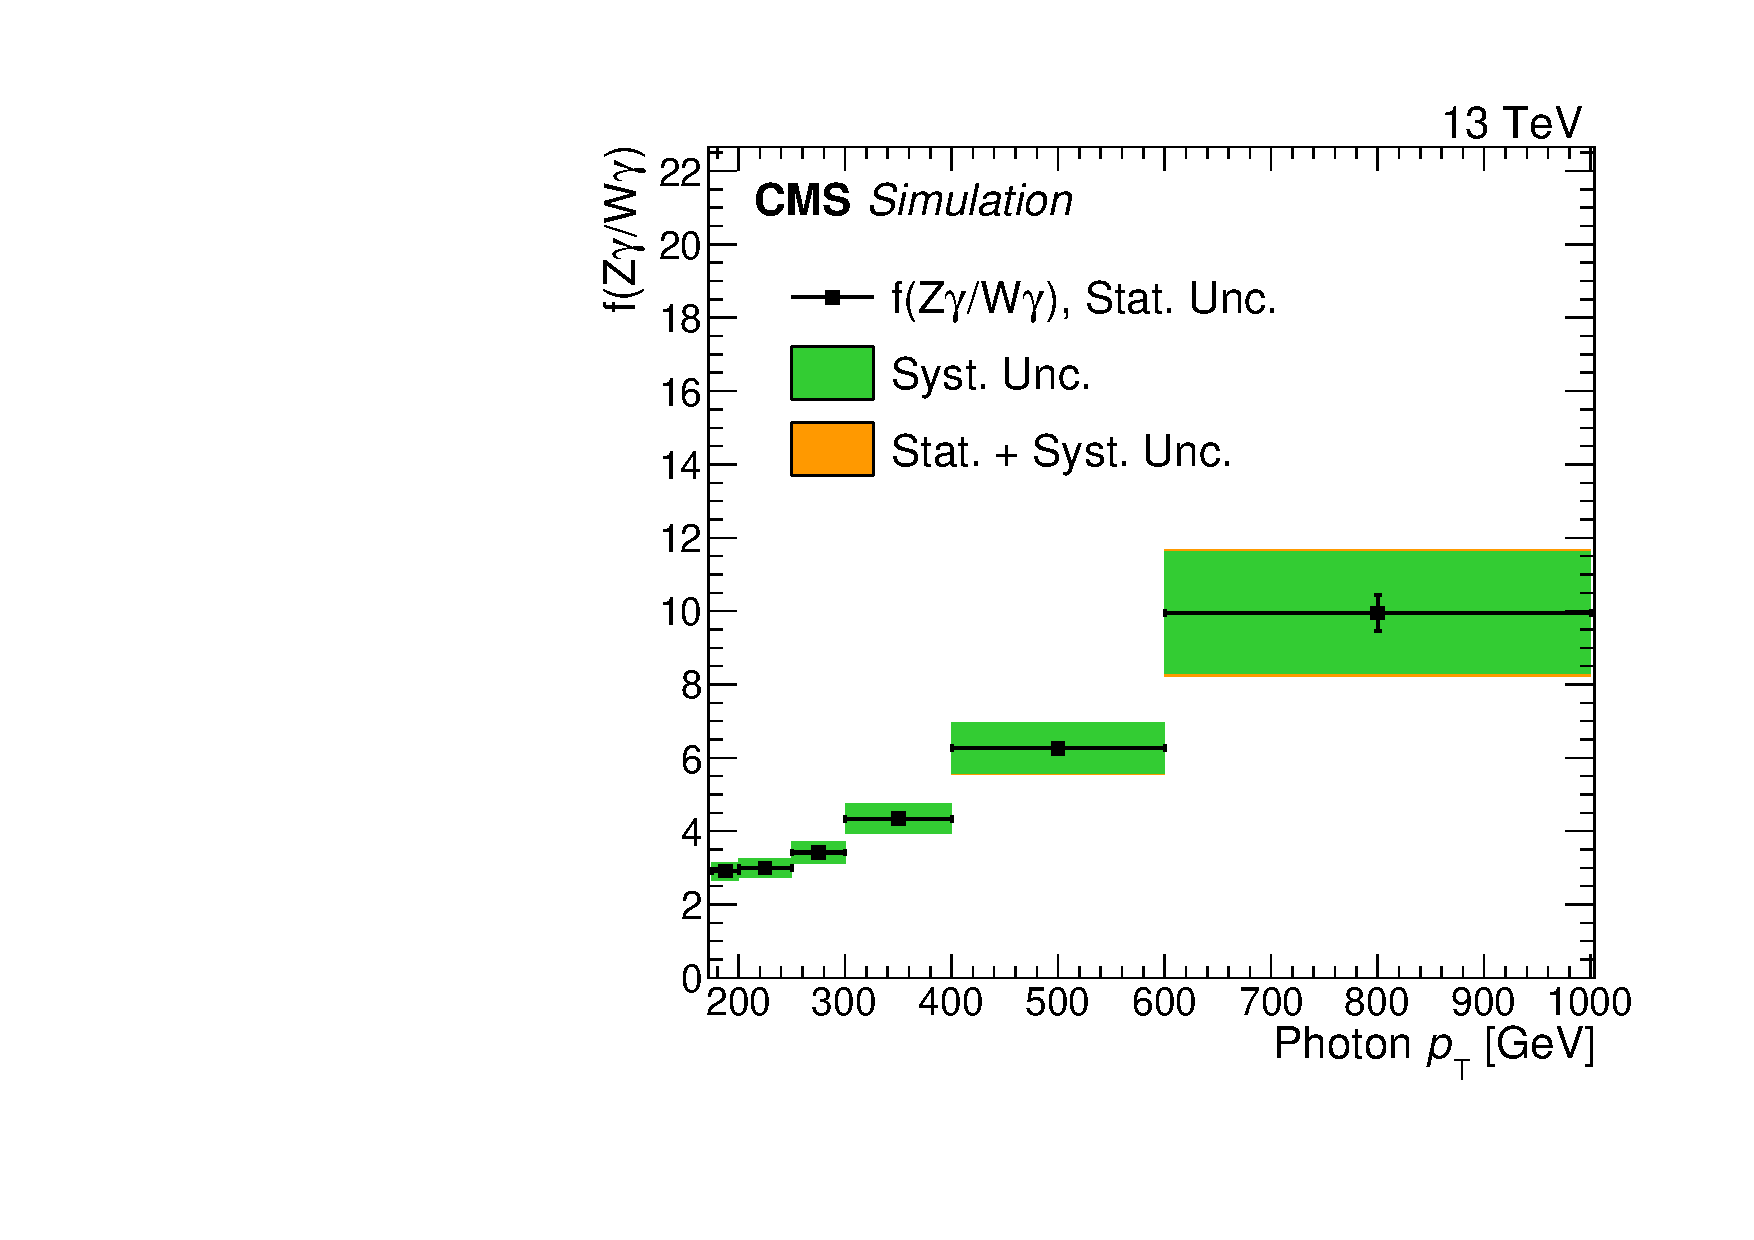
\includegraphics[width=0.45\textwidth]{figures/results/transfer_ZnnGinZnnG_over_WGinZnnG_phoPt.pdf}
    \caption{
      Transfer factor \fZW. The last bin includes all events with $\ETgamma > 1000\unit{GeV}$.
    }
    \label{fig:tf_wz}
  \end{center}
\end{figure}


The total reconstructed event yield \nl\ in each single-$\ell$ control region ($\ell \in \{e,\mu\}$) is estimated according to
\begin{equation}
  \nl[,j] = \frac{\fZW[,j]\nZg[j,all]}{\RWl[,j]} + b_{\ell\Pgamma,j}.
\end{equation}
The total reconstructed event yield \nll\ in each double-$\ell$ control region is similarly estimated according to
\begin{equation}
  \nll[,j] = \frac{\nZg[j,all]}{\RZll[,j]} + b_{\ell\ell\Pgamma,j}.
\end{equation}
where $b_{\ell\ell\Pgamma,j}$ is the estimated contribution from processes other than \zllg\ in the double-$\ell$ control region.

The complete likelihood function is
\begin{align}
  \mathcal{L} & = \left\{ \mathcal{L_{\text{Signal}}} \mathcal{L_{\text{Control}}} \right\} \times \mathcal{L_{\text{Nuisances}}} \\
  & = \prod_{j} \left\{
    \prod_{S=H,V} \mathcal{P}\left( N_{S, j} \left| \nS[,j] (\vec{\theta} \right.) \right)
     \prod_{\ell=\Pe,\Pmu} \mathcal{P}\left( N_{\ell\Pgamma, j} \left| \nl[,j] (\vec{\theta}) \right. \right)
      \prod_{\ell=\Pe,\Pmu} \mathcal{P}\left( N_{\ell\ell\Pgamma, j} \left| \nll[,j] (\vec{\theta}) \right. \right) 
    \right\}  \times \prod_{t} \mathcal{N}(\theta_t) \\
  & = \prod_{j} \left\{
  \begin{array}{cc}
    \prod\limits_{S=H,V} \mathcal{P}\left( N_{S, j} \left| C_{S} \left(\mu s_{j}(\vec{\theta}) + (1 + \fZW[,j])\nZg[j,all](\vec{\theta}) + b_{j}(\vec{\theta})\right) + h \nhalo[,j](\vec{\theta}) \right. \right) \\[1.3pt]
    \times \prod\limits_{\ell=\Pe,\Pmu} \mathcal{P}\left( N_{\ell\Pgamma, j} \left| \frac{\fZW[,j]\nZg[j,all]}{\RWl[,j](\vec{\theta})} + b_{\ell\Pgamma, j}(\vec{\theta}) \right. \right) \\[1.3pt]
    \times \prod\limits_{\ell=\Pe,\Pmu} \mathcal{P}\left( N_{\ell\ell\Pgamma, j} \left| \frac{\nZg[j,all]}{\RZll[,j](\vec{\theta})} + b_{\ell\ell\Pgamma, j}(\vec{\theta}) \right. \right) \\[1.3pt]
  \end{array} \right\}
  \times \prod_{t} \mathcal{N}(\theta_t).
\end{align}

\subsubsection{Prefit distributions}
Figures~\ref{fig:monoel}, \ref{fig:monomu}, \ref{fig:monoph_below0p5}, and Figure~\ref{fig:monoph_above0p5} show the prefit
background distributions in the single-electron, single-muon, horizontal signal region, and vertical signal region, respectively.
In these plots, the normalizations of the \zinvg, \wlng, and \zllg\ processes,
which are freely floating parameters in the fits, are assigned uncertainties corresponding to their theoretical SM cross section uncertainties.

\begin{figure}[htbp]
  \begin{center}
    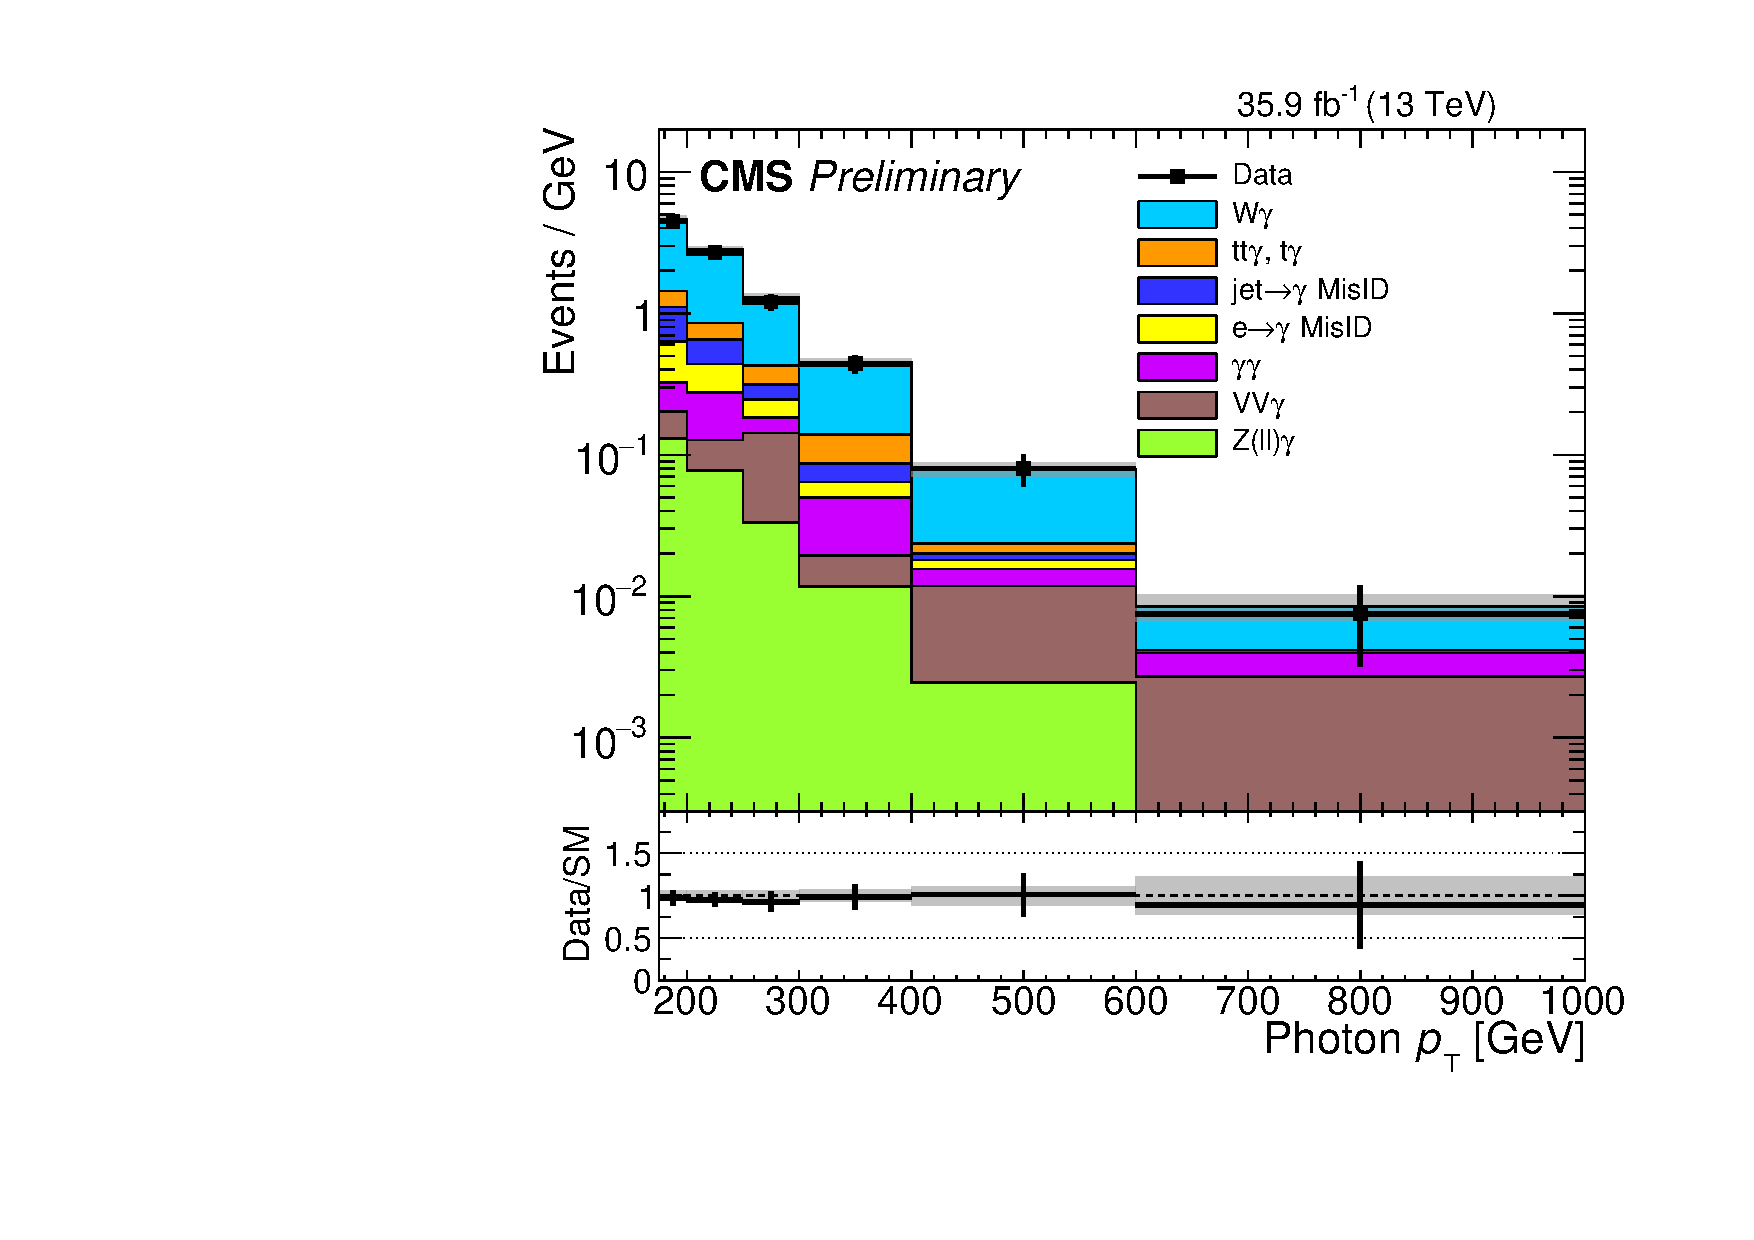
\includegraphics[width=0.45\textwidth]{Figures/results/weng_phoPt.pdf}
    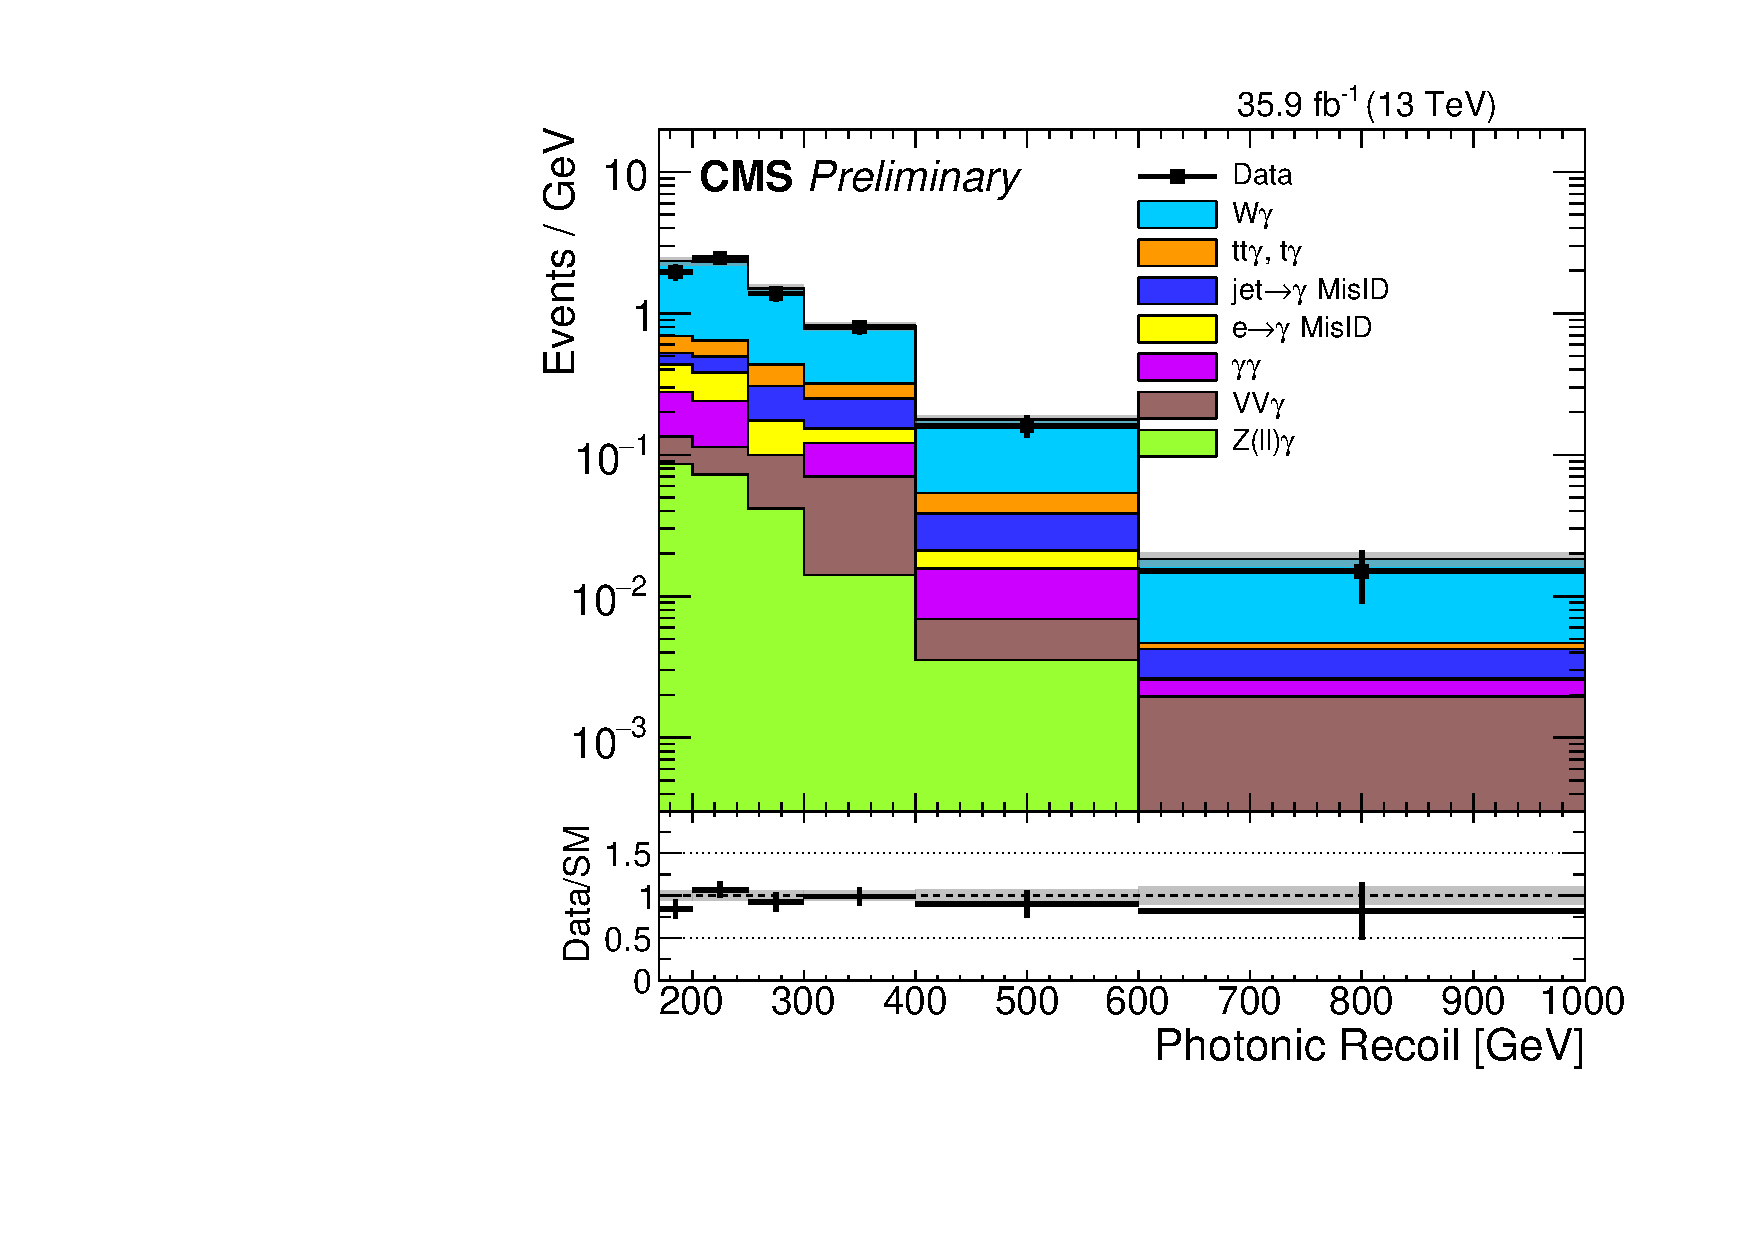
\includegraphics[width=0.45\textwidth]{Figures/results/weng_recoil.pdf}
    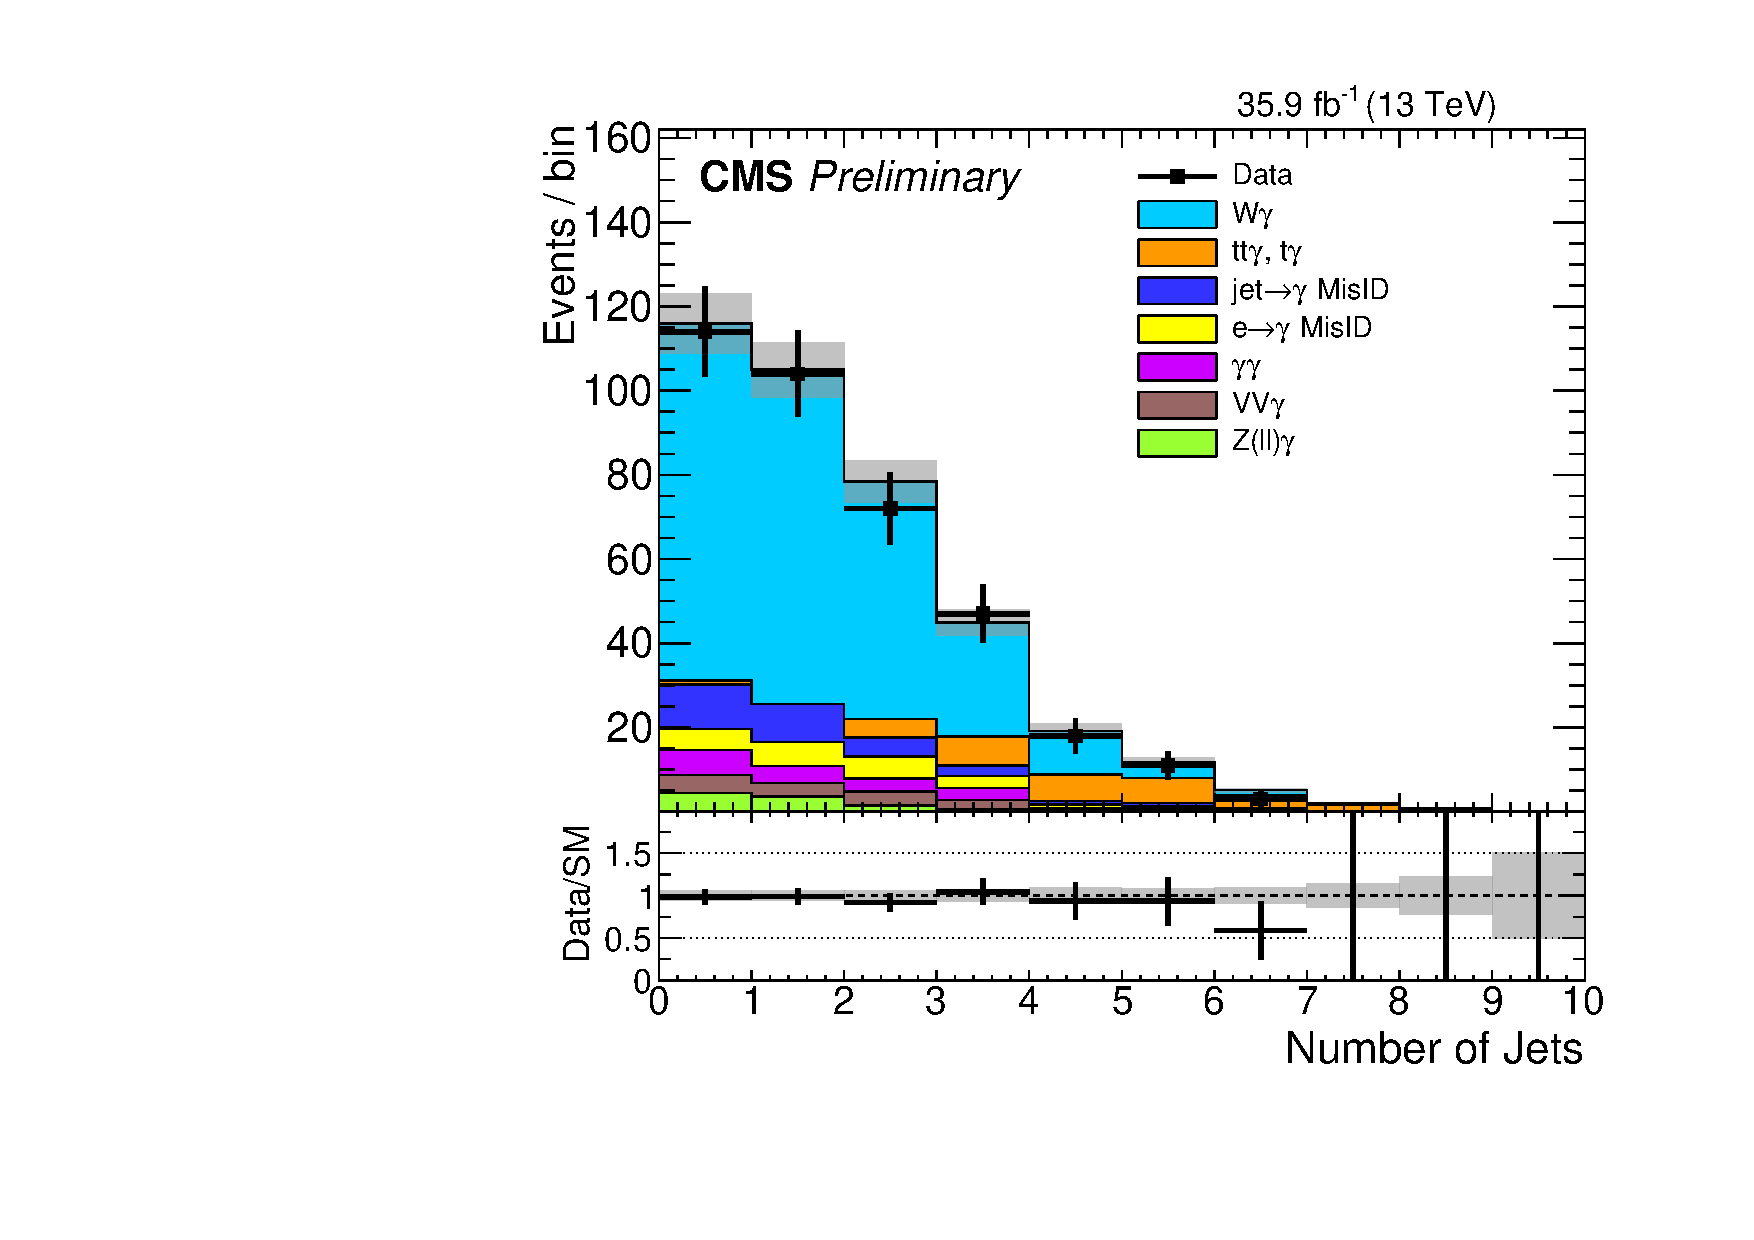
\includegraphics[width=0.45\textwidth]{Figures/results/weng_nJet.pdf}
    \caption{
      \ETgamma\ (top left), $|\vecrecoil|$ (top right), and number of jets (bottom) in the \Pe\Pgamma\ control region.
      The last bin of each distribution includes all events that fall beyond the rightmost plot boundary.
    }
    \label{fig:monoel}
  \end{center}
\end{figure}

\begin{figure}[htbp]
  \begin{center}
    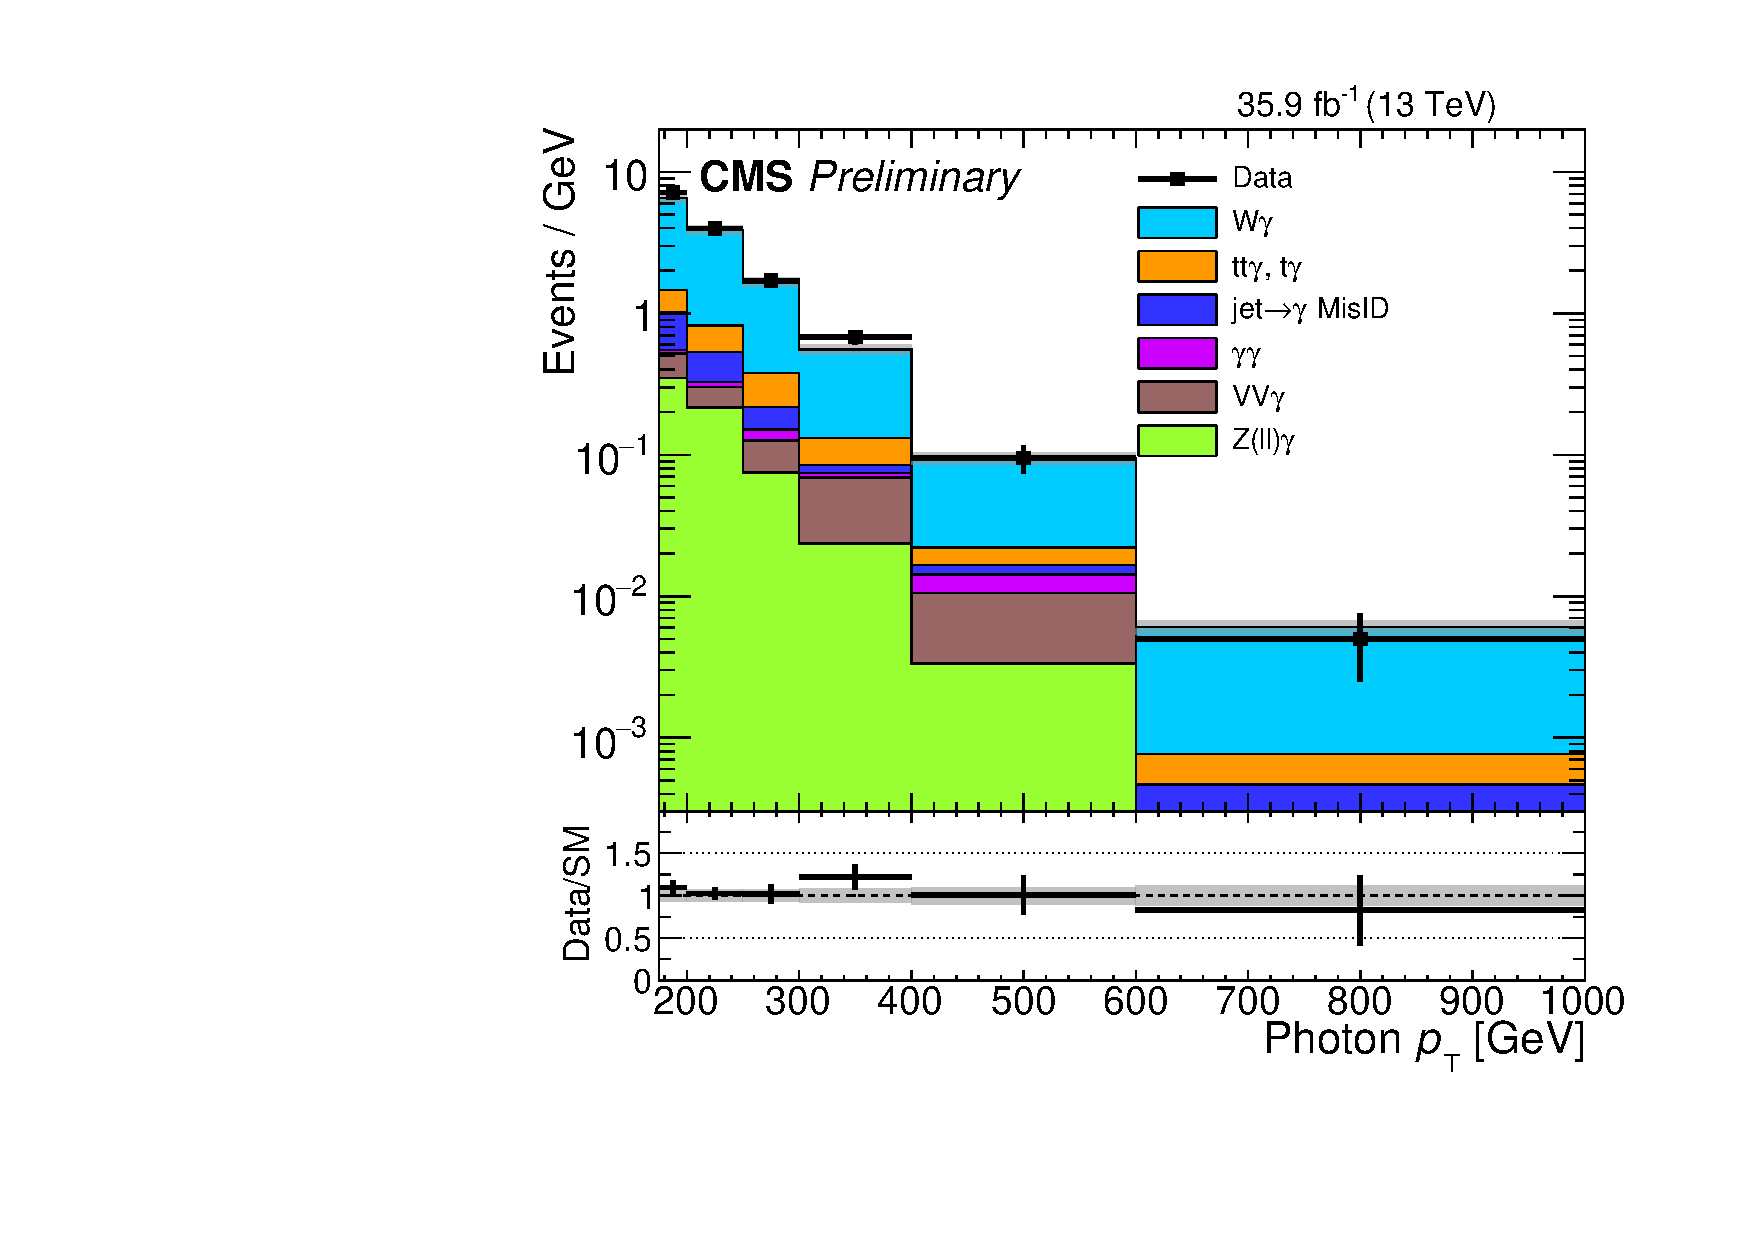
\includegraphics[width=0.45\textwidth]{Figures/results/wmng_phoPt.pdf}
    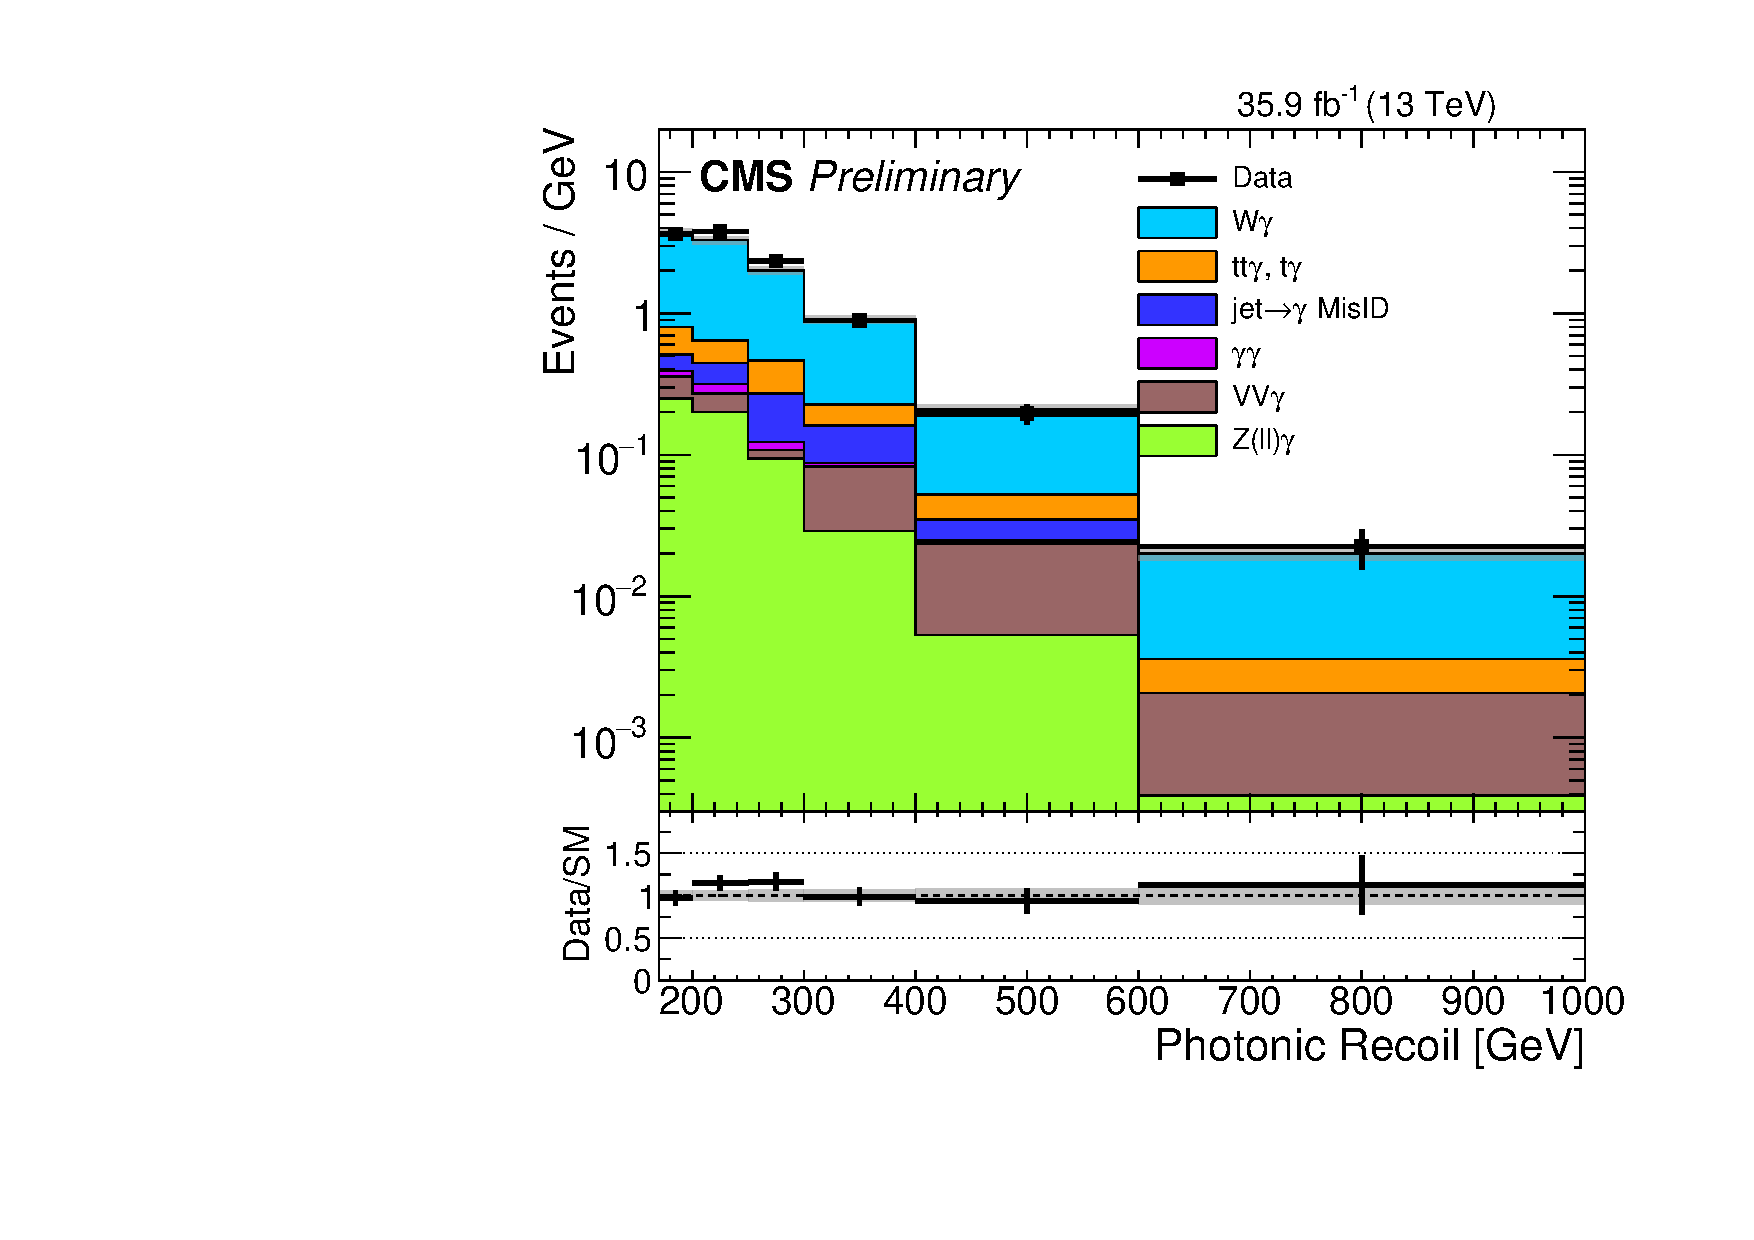
\includegraphics[width=0.45\textwidth]{Figures/results/wmng_recoil.pdf}
    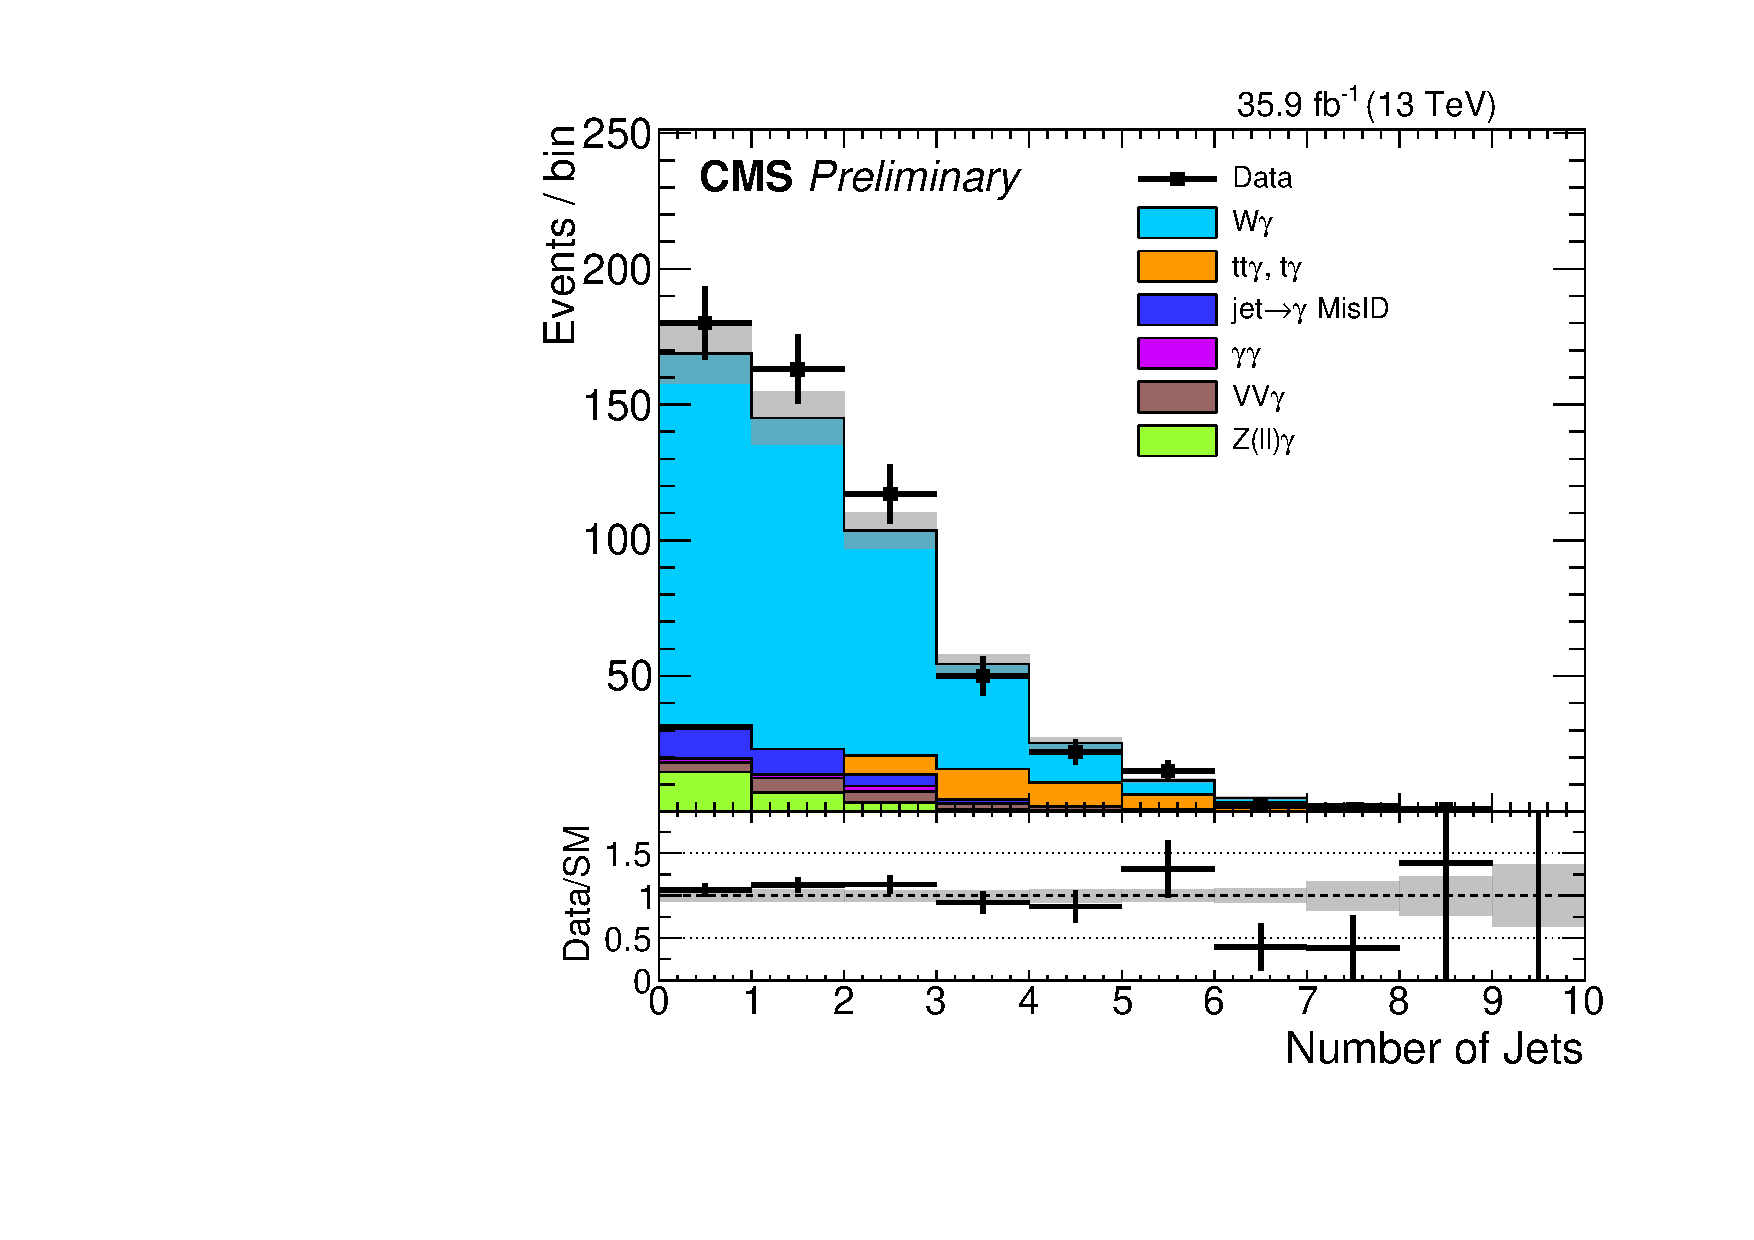
\includegraphics[width=0.45\textwidth]{Figures/results/wmng_nJet.pdf}
    \caption{
      \ETgamma\ (top left), $|\vecrecoil|$ (top right), and number of jets (bottom) in the \Pmu\Pgamma\ control region.
      The last bin of each distribution includes all events that fall beyond the rightmost plot boundary.
    }
    \label{fig:monomu}
  \end{center}
\end{figure}

\begin{figure}[htbp]
  \begin{center}
    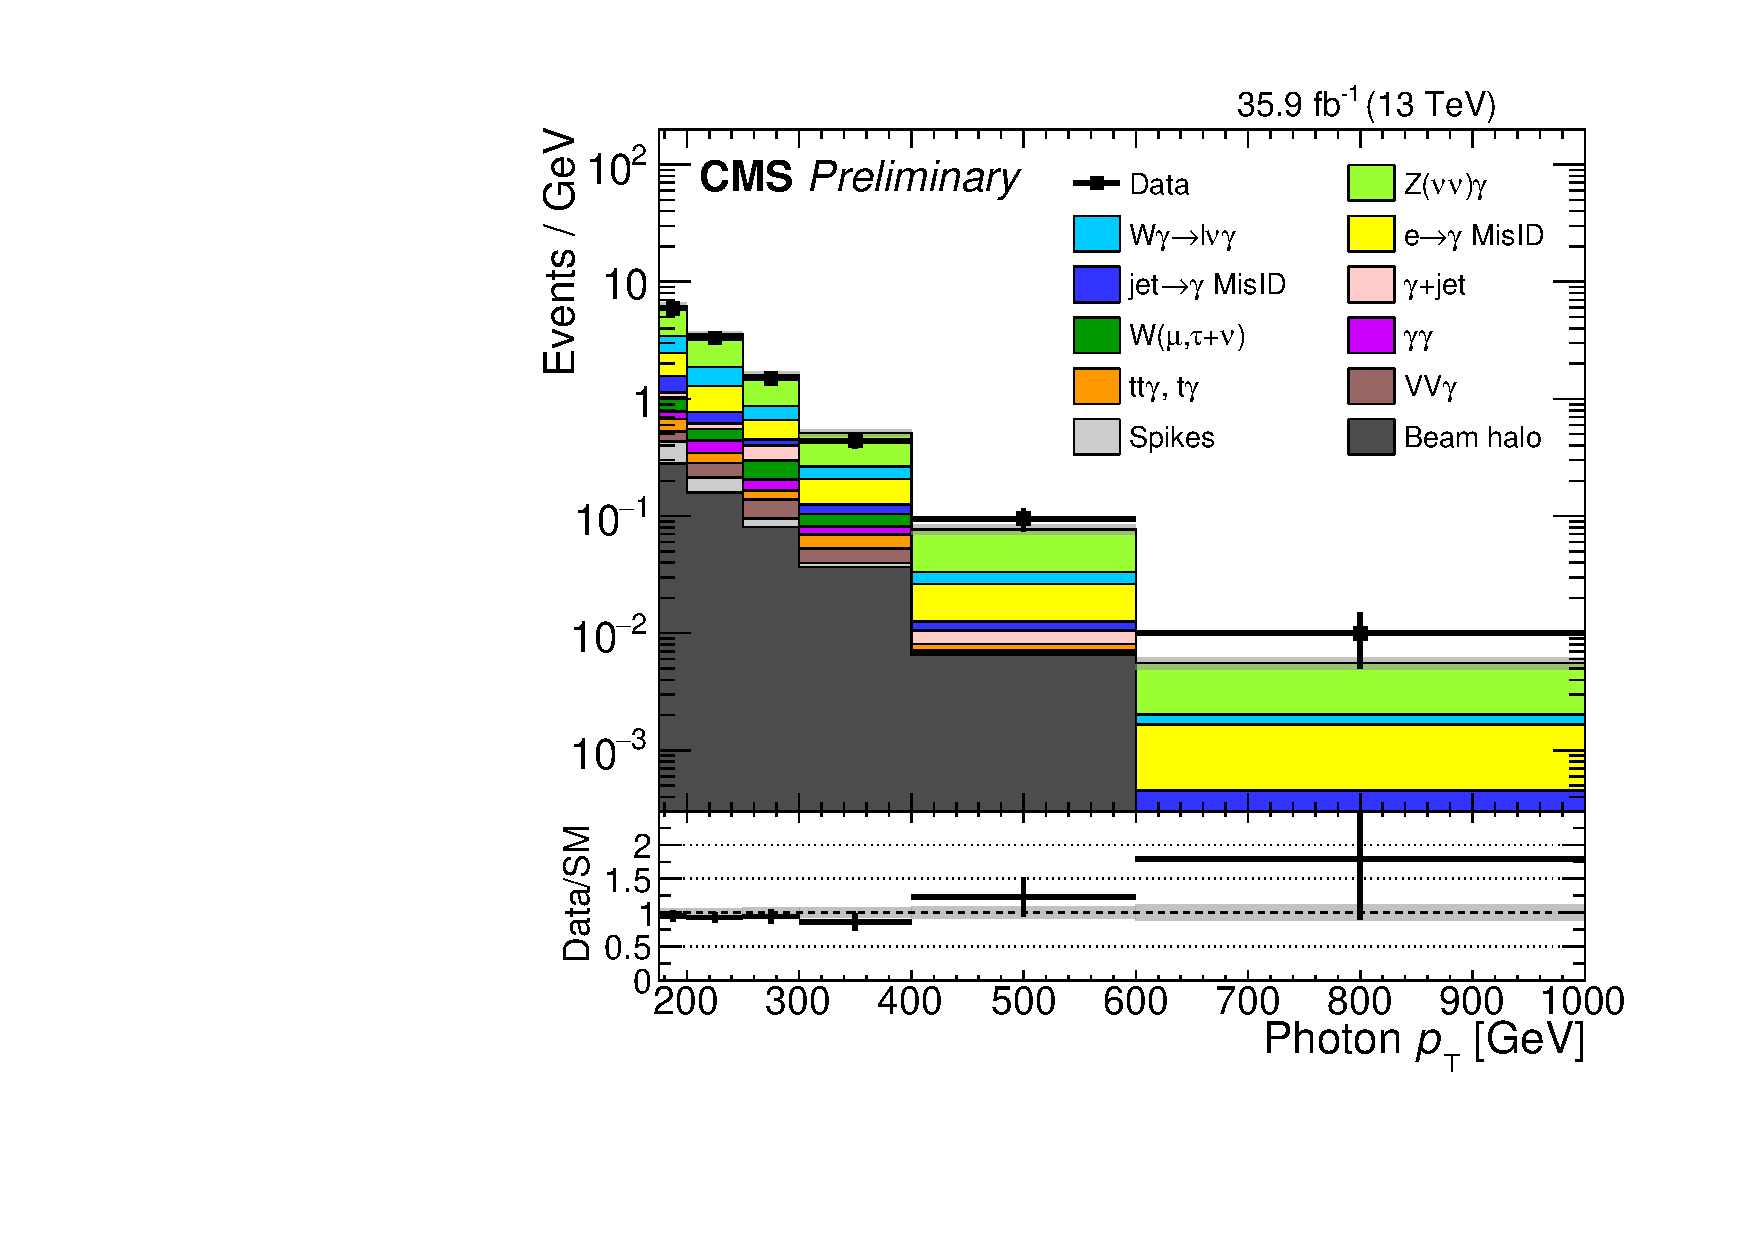
\includegraphics[width=0.45\textwidth]{Figures/results/znng_below0p5_phoPt.pdf}
    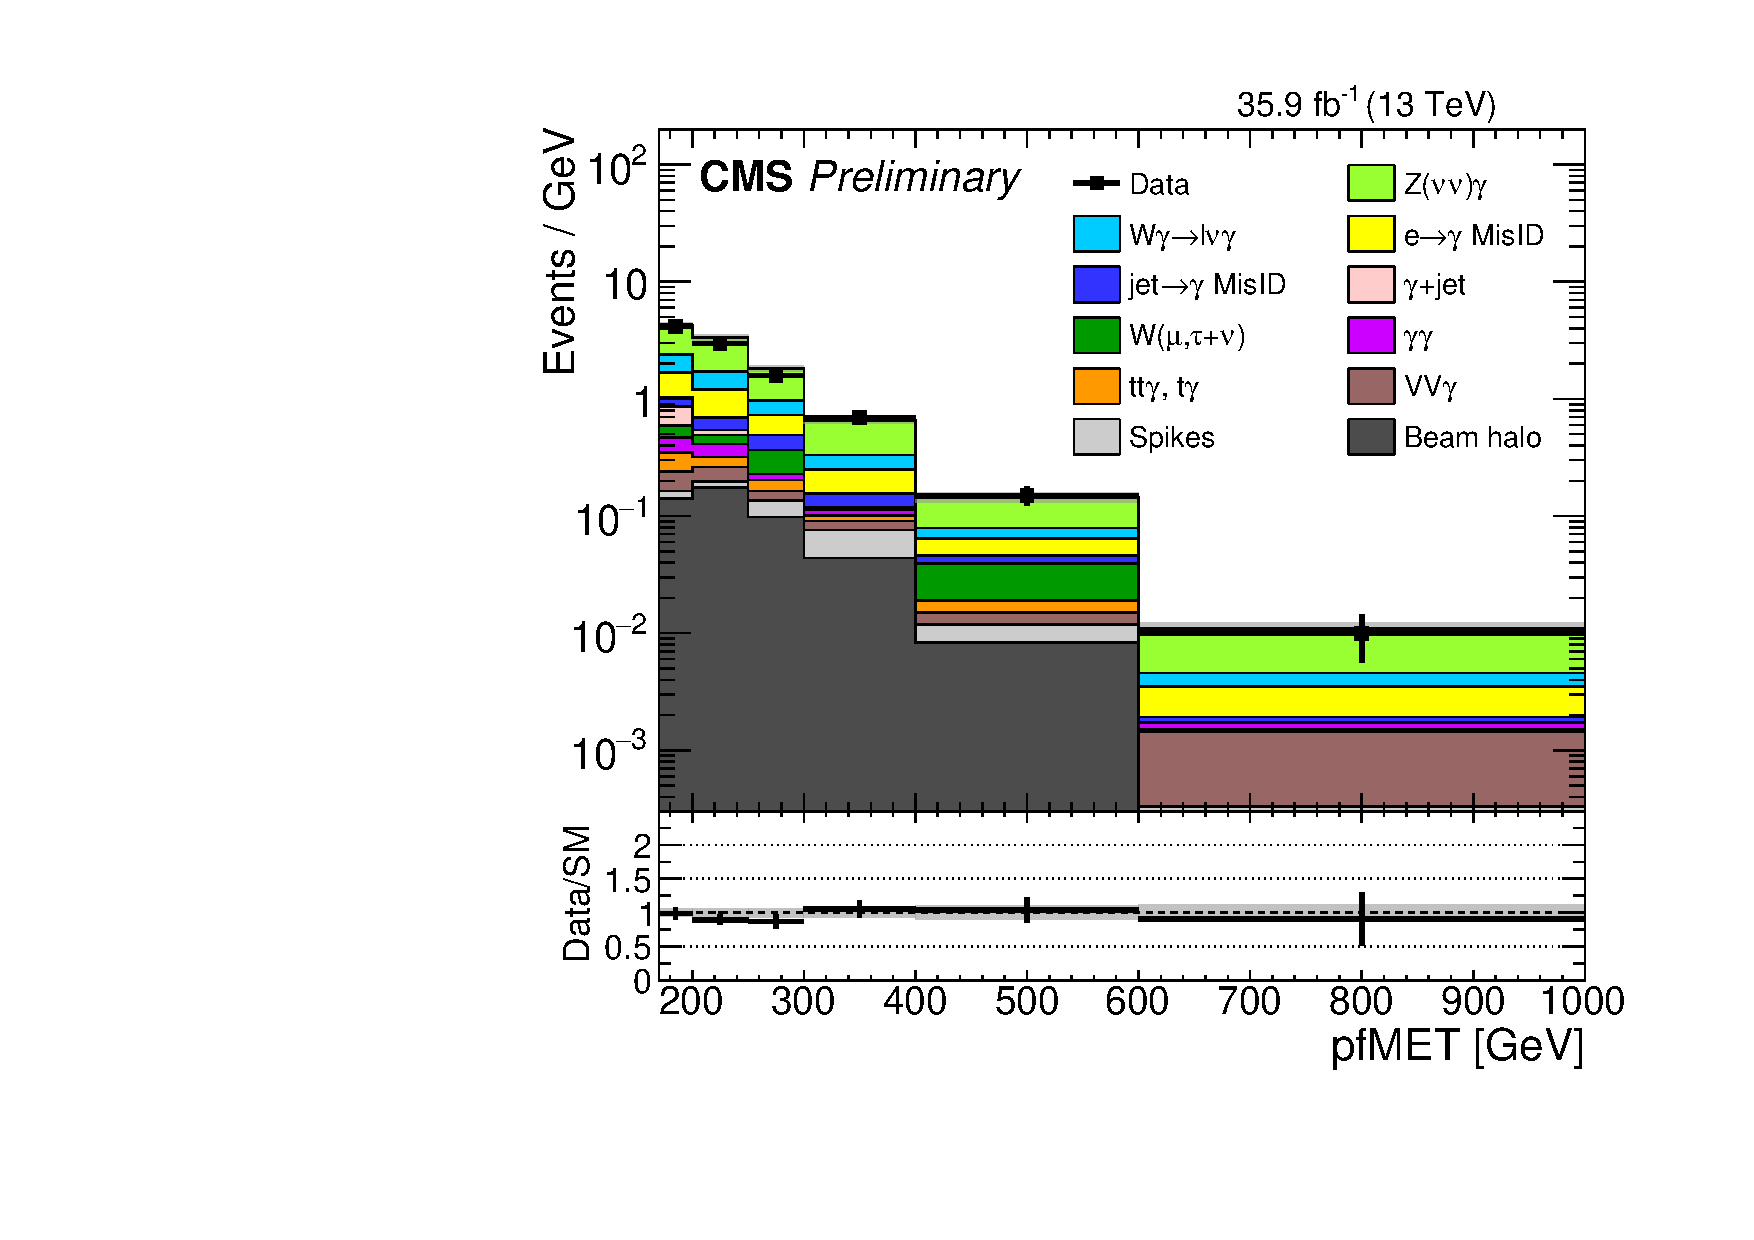
\includegraphics[width=0.45\textwidth]{Figures/results/znng_below0p5_pfMET.pdf}
    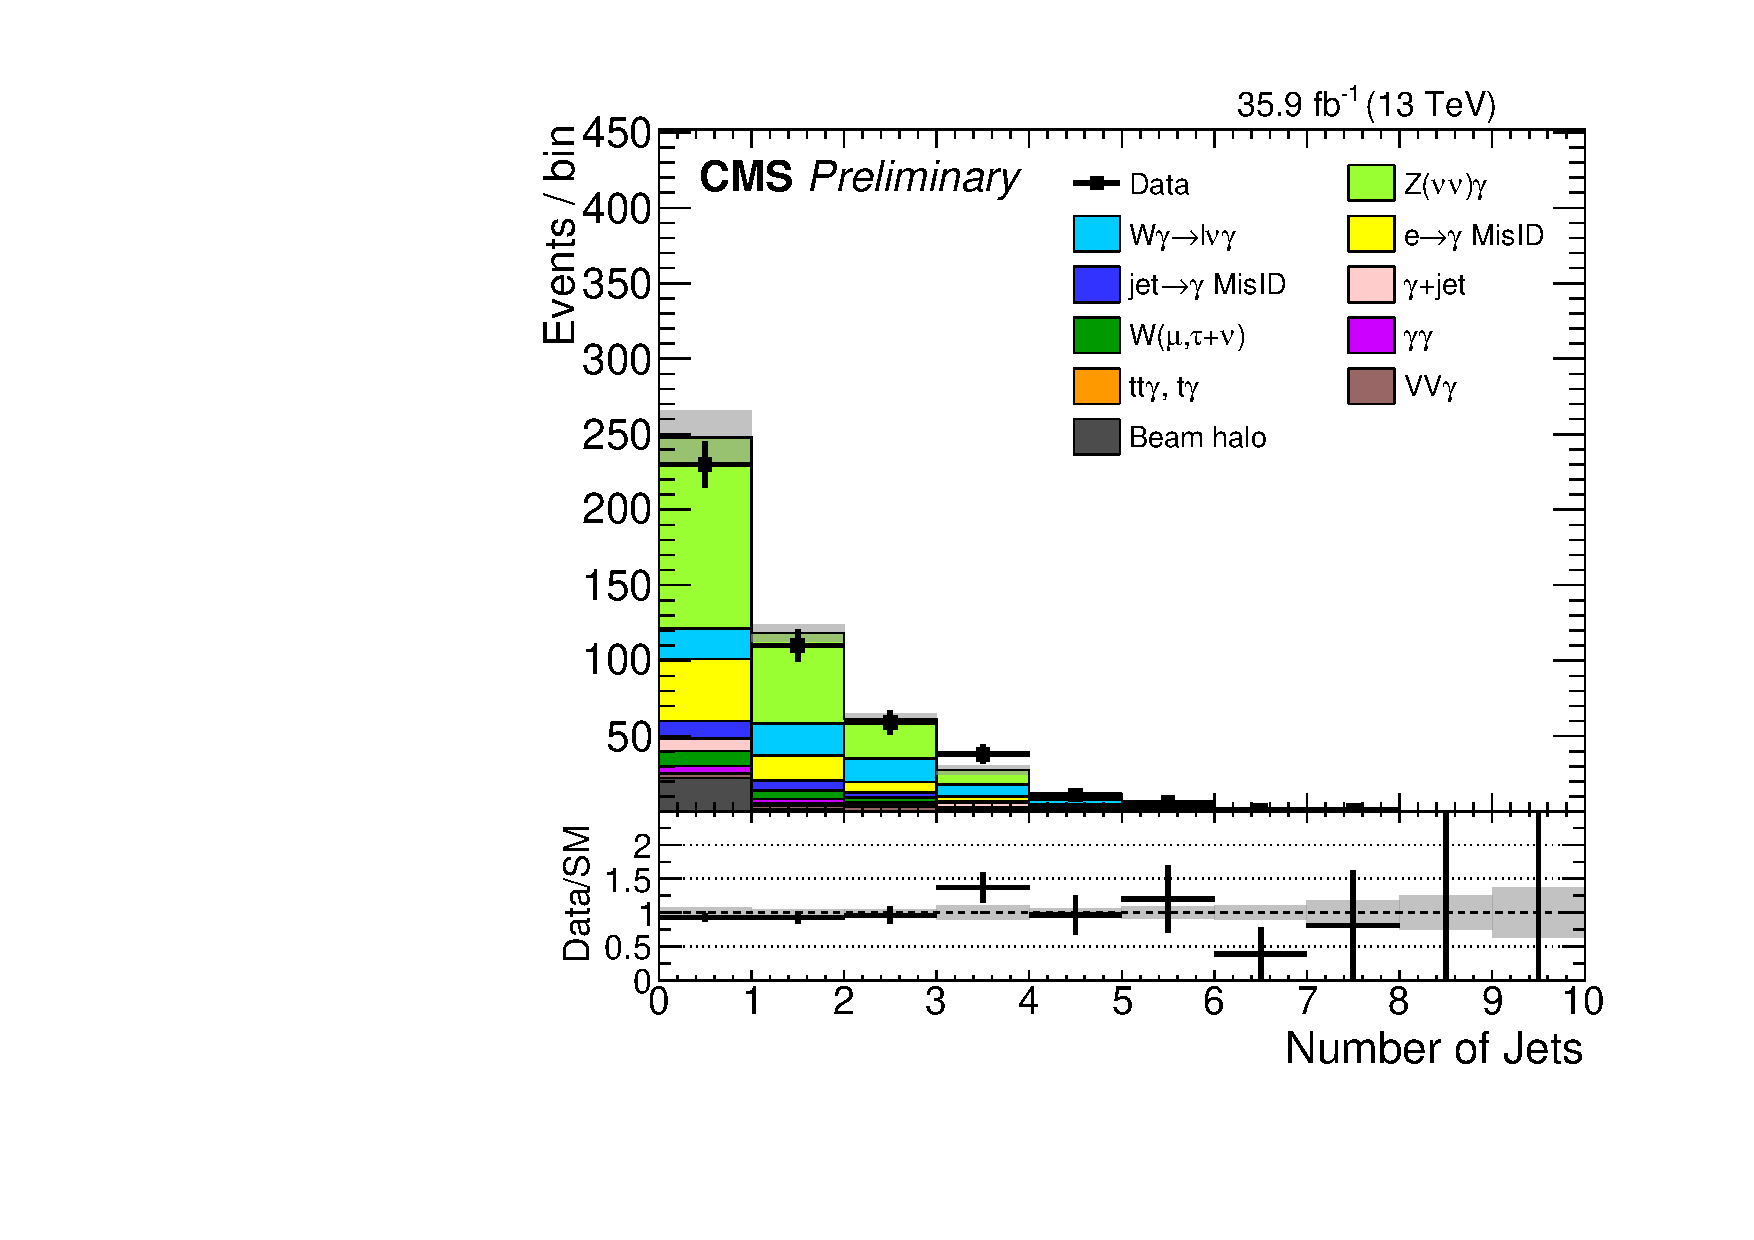
\includegraphics[width=0.45\textwidth]{Figures/results/znng_below0p5_nJet.pdf}
    \caption{
      \ETgamma\ (top left), \MET\ (top right) and number of jets (bottom) in the horizontal signal region.
      The last bin of each distribution includes all events that fall beyond the rightmost plot boundary.
    }
    \label{fig:monoph_below0p5}
  \end{center}
\end{figure}



\begin{figure}[htbp]
  \begin{center}
    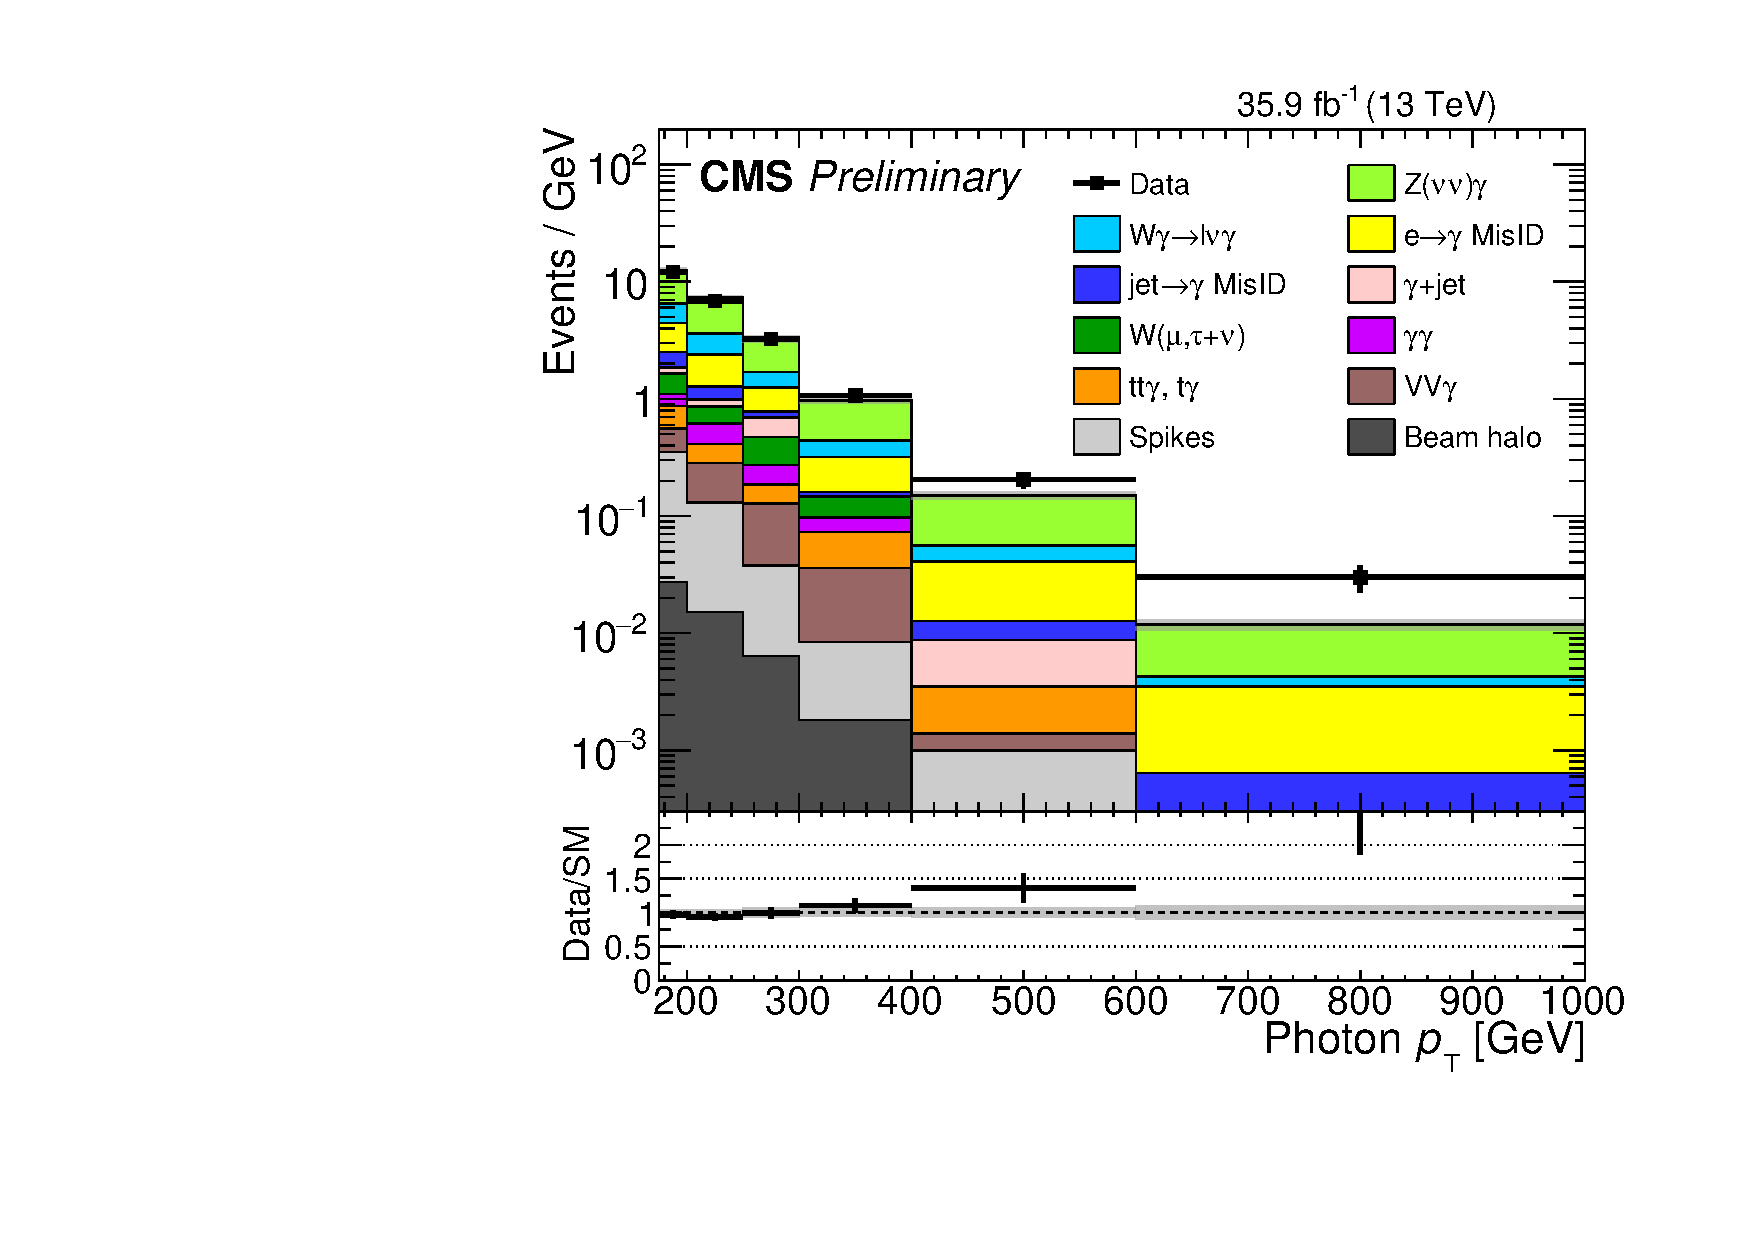
\includegraphics[width=0.45\textwidth]{Figures/results/znng_above0p5_phoPt.pdf}
    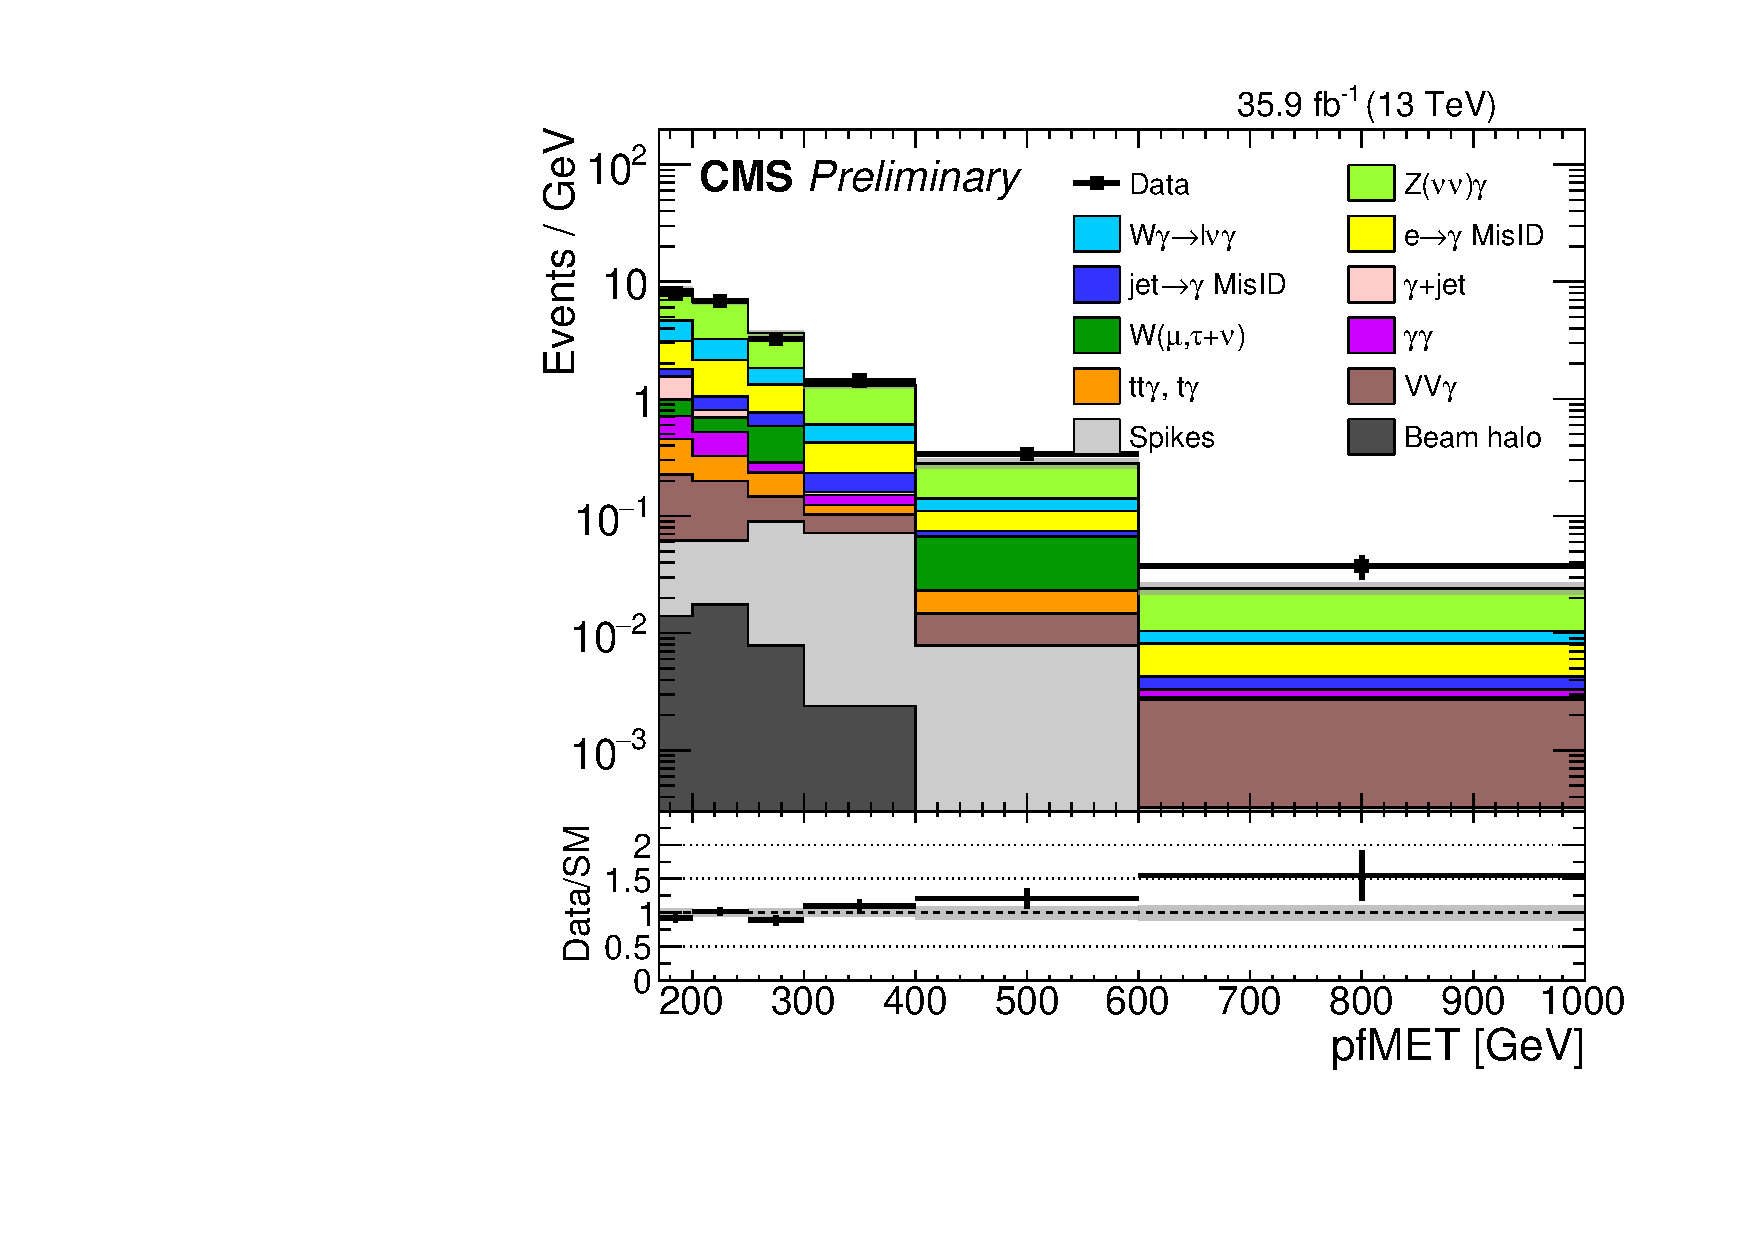
\includegraphics[width=0.45\textwidth]{Figures/results/znng_above0p5_pfMET.pdf}
    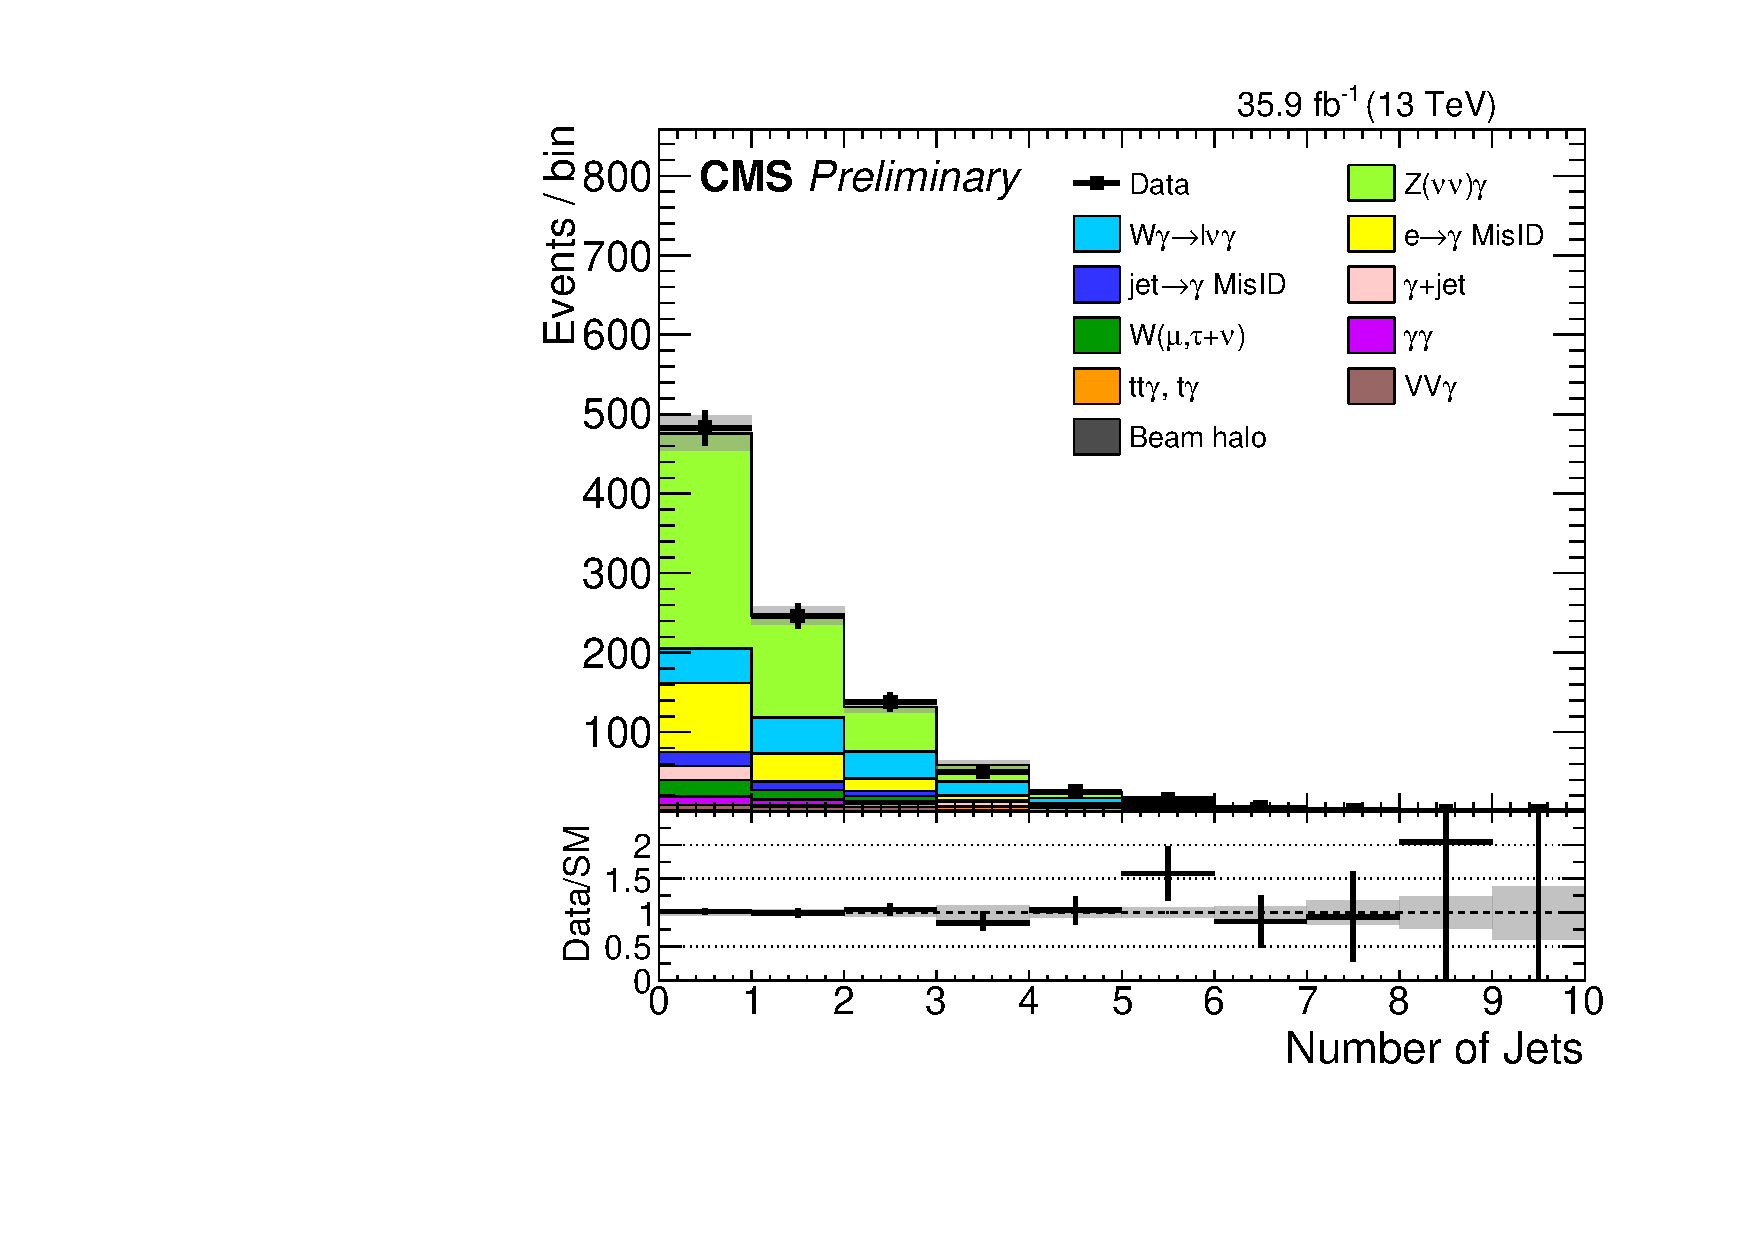
\includegraphics[width=0.45\textwidth]{Figures/results/znng_above0p5_nJet.pdf}
    \caption{
      \ETgamma\ (top left), \MET\ (top right) and number of jets (bottom) in the vertical signal region.
      The last bin of each distribution includes all events that fall beyond the rightmost plot boundary.
    }
    \label{fig:monoph_above0p5}
  \end{center}
\end{figure}

